% \documentclass[8pt,adobefonts,fancyhdr,hyperref,UTF8]{ctexbook}
\documentclass[10pt,fancyhdr,hyperref,UTF8]{ctexbook}

\usepackage{multirow}
% for \soul 删除线
\usepackage{ulem}
% 表头斜线
\usepackage{diagbox}

\makeatletter
\usepackage[centering,paperwidth=180mm,paperheight=230mm,%
body={390pt,530pt},marginparsep=10pt,marginpar=50pt]{geometry}
\usepackage{color}
\usepackage{enumitem}
\usepackage{fancyvrb}
\usepackage[bottom,perpage,symbol*]{footmisc}
\usepackage{graphicx}
\usepackage[hidelinks]{hyperref}
\usepackage{makeidx}
\usepackage[toc]{multitoc}
\usepackage{pifont}
\usepackage{underscore}
\usepackage{amsmath}

\DefineFNsymbols*{chinese}{{\ding{172}}{\ding{173}}{\ding{174}}{\ding{175}}%
{\ding{176}}{\ding{177}}{\ding{178}}{\ding{179}}{\ding{180}}{\ding{181}}}
\setfnsymbol{chinese}

\hypersetup{bookmarksnumbered=true,bookmarksdepth=2}

\CTEXsetup[number={\thechapter}]{chapter}
\CTEXsetup[format+={\raggedleft}]{chapter}
\CTEXsetup[beforeskip={10pt}]{chapter}
\CTEXsetup[afterskip={30pt}]{chapter}
\def\CTEX@chapter@aftername{\par} % \CTEXsetup[aftername={\par}]{chapter}
\CTEXsetup[format+={\raggedright}]{section}
\CTEXsetup[beforeskip={-3.0ex plus -1ex minus -.2ex}]{section}
\CTEXsetup[afterskip={2.3ex plus .2ex minus 0.2ex}]{section}

\renewcommand \thefigure{\thechapter-\arabic{figure}}
\renewcommand \thetable{\thechapter-\arabic{table}}

\newcommand\figcaption[1]{\def\@captype{figure}\caption{#1}}
\newcommand\tabcaption[1]{\def\@captype{table}\caption{#1}}

\long\def\@caption#1[#2]#3{%
  \addcontentsline{\csname ext@#1\endcsname}{#1}%
    {\protect\numberline{\csname fnum@#1\endcsname}{ \ignorespaces #2}}% change "the" to "fnum@"
    \normalsize
    \@makecaption{\csname fnum@#1\endcsname}{\ignorespaces #3}}

\long\def\@makecaption#1#2{%
  \vskip\abovecaptionskip
  \sbox\@tempboxa{#1\quad#2}%
  \ifdim \wd\@tempboxa >\hsize
    #1\quad#2\par
  \else
    \global \@minipagefalse
    \hb@xt@\hsize{\hfil\box\@tempboxa\hfil}%
  \fi
  \vskip\belowcaptionskip}

\setlength\abovecaptionskip{0pt}
  
%\setmainfont{Times New Roman}
\setmainfont{Linux Libertine O}
%\setmainfont{TeX Gyre Pagella}
\newfontfamily\urlfont{PT Sans Narrow}
%\setmonofont[AutoFakeBold=1.6,AutoFakeSlant=0.17,Mapping=tex-text-tt]{Inconsolata}
\setCJKfamilyfont{zhyou}{YouYuan}

\newcommand{\fn}[1]{\texttt{#1}}
\newcommand{\sfn}[1]{\texttt{\small #1}}
\newcommand{\kw}[1]{\textsf{#1}}
\newcommand{\myurl}[1]{{\urlfont #1}}
\newcommand{\mpar}[1]{\marginpar[\hfill\kaishu #1]{\kaishu #1}}
\newcommand{\mn}[1]{\texttt{\bs #1}}
\renewcommand{\today}{\the\year-\the\month-\the\day}
\newcommand\bs{\textbackslash}

\newcommand\begindot{\begin{itemize}
[itemsep=2pt plus 2pt minus 2pt,%
topsep=3pt plus 2pt minus 2pt,%
parsep=0pt plus 2pt minus 2pt]}
\newcommand\myenddot{\end{itemize}}

\newcommand\beginnum{\begin{enumerate}
[itemsep=2pt plus 2pt minus 2pt,%
topsep=3pt plus 2pt minus 2pt,%
parsep=0pt plus 2pt minus 2pt]}
\newcommand\myendnum{\end{enumerate}}

\DefineVerbatimEnvironment%
  {Code}{Verbatim}
  {fontsize=\small,baselinestretch=0.9,xleftmargin=3mm}

\raggedbottom
%\setlength{\parskip}{1ex plus .5ex minus .5ex}

\input{verbatim.cls}
\DefineVerbatimEnvironment%
  {Codex}{Verbatim}
  {fontsize=\small,baselinestretch=0.9,xleftmargin=3mm,%
  frame=lines,labelposition=all,framesep=5pt}

\DefineVerbatimEnvironment%
  {Code}{Verbatim}
  {fontsize=\small,baselinestretch=0.9,xleftmargin=3mm}

\makeindex
\makeatother

%--------------------------------------------------------------
\usepackage{color}
\newcommand{\Note}[1]{\textcolor{blue}{【注:#1】}} %% 笔记
\newcommand{\Hl}[1]{\textcolor{red}{#1}} %% Highlight
\newcommand{\Dl}{---------------------------------------------------------------------分割线-------------------------------------------------------------------} %% Dividingline
\usepackage{listings}
\lstnewenvironment{NoteCode}{
\lstset{ %
backgroundcolor=\color{white},   % choose the background color
basicstyle=\small,        % size of fonts used for the code
columns=fullflexible,
breaklines=true,                 % automatic line breaking only at whitespace
captionpos=b,                    % sets the caption-position to bottom
tabsize=4,
commentstyle=\color{magenta},    % comment style
escapeinside={\%*}{*)},          % if you want to add LaTeX within your code
keywordstyle=\color{blue},       % keyword style
stringstyle=\color{green}\ttfamily,     % string literal style
frame=single, % none
% rulesepcolor=\color{red!20!green!20!blue!20},
% identifierstyle=\color{red},
language=C++
}}{}

%---------------------------上面的现实注释,下面的不现实注释---------------

% \newcommand{\Note}[1]{} %% 笔记 (注释掉)
% \newcommand{\Hl}[1]{#1} %% Highlight (注释掉)
% \newcommand{\Dl}[1]{} %% Dividingline (注释掉)
% \usepackage{comment}
% \newenvironment{NoteCode}{}{}
% \excludecomment{NoteCode}
%-------------------------------------------------------------



\begin{document}
\sloppy
\newcommand\BookTitle{手写代码必备手册}
\pagestyle{fancy}
\fancyhf{}
\fancyhead[RE]{\normalfont\small\rmfamily\nouppercase{\leftmark}}
\fancyhead[LO]{\normalfont\small\rmfamily\nouppercase{\rightmark}}
\fancyhead[LE,RO]{\thepage}
%\fancyfoot[LE,LO]{\small\normalfont\youyuan\BookTitle}
%\fancyfoot[RE,RO]{\textsf{\small \color{blue} https://github.com/soulmachine/acm-cheatsheet}}

\makeatletter
\@openrightfalse
\makeatother

\frontmatter % 开始前言目录,页码用罗马数字

% \include{title}

\tableofcontents

\mainmatter % 开始正文,页码用阿拉伯数字

\graphicspath{{diagrams/}}

% \chapter{编程技巧}
把\Hl{较大的数组放在main函数外,作为全局变量,这样可以防止栈溢出,} 因为栈的大小是有限制的。

如果能够预估栈,队列的上限,则不要用\fn{stack, queue},使用数组来模拟,这样速度最快。

输入数据一般放在全局变量,且在运行过程中不要修改这些变量。\Note{减少传参}

在判断两个浮点数a和b是否相等时,不要用\fn{a==b},应该判断二者之差的绝对值\fn{fabs(a-b)}是否小于某个阈值,例如\fn{1e-9}。 \Note{误差限制}

判断一个整数是否是为奇数,用\fn{x \% 2 != 0},\Hl{不要用\fn{x \% 2 == 1},因为x可能是负数。}

用\fn{char}的值作为数组下标(例如,统计字符串中每个字符出现的次数),要考虑到\fn{char}可能是负数。有的人考虑到了,先强制转型为\fn{unsigned int}再用作下标,这仍然是错的。正确的做法是,\Hl{先强制转型为\fn{unsigned char},再用作下标。}这涉及C++整型提升的规则,就不详述了。\Note{1字节$\rightarrow$4字节:有符号数据类型:正数填充0,负数填充1;无符号数据类型:填充0}

% \chapter{线性表}
线性表(Linear List)包含以下几种:
\begindot
\item 顺序存储:数组
\item 链式存储:单链表,双向链表,循环单链表,循环双向链表
\item 二者结合:静态链表
\myenddot

\Note{
std::array Defined in header <array>
}
\begin{NoteCode}
template <class Ty, std::size_t N>
class array;
\end{NoteCode}

\Note{\\
\textbf{parameters}: \\
\fn{Ty} 元素的类型; \\
\fn{N} 元素数量。\\
\\
\textbf{Members}: \\
\underline{const_iterator}	The type of a constant iterator for the controlled sequence.( \fn{for (Array::const_iterator it = a.begin(); it != a.end(); ++it);} )\\
\underline{const_pointer}	The type of a constant pointer to an element. ( \fn{Array::const_pointer ptr = \&*a.begin();} ) \\
\underline{const_reference}	The type of a constant reference to an element. ( \fn{Array::const_reference ref = *a.begin();} )\\
\underline{const_reverse_iterator}	The type of a constant reverse iterator for the controlled sequence. ( \fn{Array::const_reverse_iterator it = a.rbegin();} ) \\
\underline{difference_type}	The type of a signed distance between two elements. ( \fn{Array::difference_type diff = a.begin() - a.end();} )\\
\underline{iterator}	The type of an iterator for the controlled sequence. ( \fn{for (Array::iterator it = a.begin(); it != a.end(); ++it)} ) \\
\underline{pointer}	The type of a pointer to an element. ( \fn{Array::pointer ptr = \&*a.begin();} ) \\
\underline{reference}	The type of a reference to an element. (\fn{Array::reference ref = *a.begin();} ) \\
\underline{reverse_iterator}	The type of a reverse iterator for the controlled sequence. ( \fn{Array::reverse_iterator it = a.rbegin();} ) \\
\underline{size_type}	The type of an unsigned distance between two elements. ( \fn{Array::size_type diff = a.end() - a.begin();} ) \\
\underline{value_type}	The type of an element. (\fn{Array::value_type val = *a.begin();}) \\
\\
\textbf{Member Function}: \\
\underline{array}	Constructs an array object. \\
\underline{assign}	(Obsolete. Use fill.) Replaces all elements. \\
\underline{at}	Accesses an element at a specified position. ( \fn{a.at(1);} ) \\
\underline{back}	Accesses the last element. \\
\underline{begin}	Designates the beginning of the controlled sequence. \\
\underline{cbegin}	Returns a random-access const iterator to the first element in the array. \\
\underline{cend}	Returns a random-access const iterator that points just beyond the end of the array. \\
\underline{crbegin}	Returns a const iterator to the first element in a reversed array. \\
\underline{crend}	Returns a const iterator to the end of a reversed array. \\
\underline{data}	Gets the address of the first element. \\
\underline{empty}	Tests whether elements are present. \\
\underline{end}	Designates the end of the controlled sequence. \\
\underline{fill}	Replaces all elements with a specified value. \\
\underline{front}	Accesses the first element. \\
\underline{max_size}	Counts the number of elements. \\
\underline{rbegin}	Designates the beginning of the reversed controlled sequence. \\
\underline{rend}	Designates the end of the reversed controlled sequence. \\
\underline{size}	Counts the number of elements. \\
\underline{swap}	Swaps the contents of two containers. \\
\\
\textbf{Operator}:\\
\underline{array::operator=}	Replaces the controlled sequence.\\
\underline{array::operator[]}	Accesses an element at a specified position.\\
}

\Dl

\Note{
std::vector Defined in header <vector>
}

\begin{NoteCode}
template <class Type, class Allocator = allocator<Type>>
class vector
\end{NoteCode}

\Note{
\textbf{Member functions}\\
\underline{assign}	Erases a vector and copies the specified elements to the empty vector.\\
\underline{at}	Returns a reference to the element at a specified location in the vector.\\
\underline{back}	Returns a reference to the last element of the vector.\\
\underline{begin}	Returns a random-access iterator to the first element in the vector.\\
\underline{capacity}	Returns the number of elements that the vector could contain without allocating more storage.\\
\underline{cbegin}	Returns a random-access const iterator to the first element in the vector.\\
\underline{cend}	Returns a random-access const iterator that points just beyond the end of the vector.\\
\underline{crbegin}	Returns a const iterator to the first element in a reversed vector.\\
\underline{crend}	Returns a const iterator to the end of a reversed vector.\\
\underline{clear}	Erases the elements of the vector.\\
\underline{data}	Returns a pointer to the first element in the vector.\\
\underline{emplace}	Inserts an element constructed in place into the vector at a specified position. ( \fn{vv1.emplace( vv1.begin(), move( vector <int>(1,2) ) );} ) \\
\underline{emplace_back}	Adds an element constructed in place to the end of the vector. ( \fn{v.emplace_back(1, 3.14);} ) \\
\underline{empty}	Tests if the vector container is empty.\\
\underline{end}	Returns a random-access iterator that points to the end of the vector.\\
\underline{erase}	Removes an element or a range of elements in a vector from specified positions. ( \fn{iterator erase(const_iterator position); \\
iterator erase(const_iterator first,const_iterator last);} ) \\
\underline{front}	Returns a reference to the first element in a vector.\\
\underline{get_allocator}	Returns an object to the allocator class used by a vector.\\
\underline{insert}	Inserts an element or many elements into the vector at a specified position.( \fn{\\iterator insert(const_iterator position, const Type\& value);\\
iterator insert(const_iterator position, Type\&\& value);\\
void insert(const_iterator position, size_type count, const Type\& value);\\
template <class InputIterator>
void insert(const_iterator position, InputIterator first,InputIterator last);
} )\\
\underline{max_size}	Returns the maximum length of the vector.\\
\underline{pop_back}	Deletes the element at the end of the vector.\\
\underline{push_back}	Add an element to the end of the vector.\\
\underline{rbegin}	Returns an iterator to the first element in a reversed vector.\\
\underline{rend}	Returns an iterator to the end of a reversed vector.\\
\underline{reserve}	Reserves a minimum length of storage for a vector object.\\
\underline{resize}	Specifies a new size for a vector.\\
\underline{shrink_to_fit}	Discards excess capacity.(丢弃空闲内存)\\
\underline{size} Returns the number of elements in the vector.\\
\underline{swap}	Exchanges the elements of two vectors.\\
}


\Dl

\Note{std::deque Defined in header <deque>}

\begin{NoteCode}
template <class Type, class Allocator =allocator<Type>>
class deque
\end{NoteCode}

\Note{
\\
\textbf{Member functions}\\
$\cdots$\\
\underline{emplace}	Inserts an element constructed in place into the deque at a specified position.\\
\underline{emplace_back}	Adds an element constructed in place to the end of the deque.\\
\underline{emplace_front}	Adds an element constructed in place to the start of the deque.\\
\underline{insert}	Inserts an element, several elements, or a range of elements into the deque at a specified position.\\
\underline{max_size}	Returns the maximum possible length of the deque.\\
\underline{pop_back}	Erases the element at the end of the deque.\\
\underline{pop_front}	Erases the element at the start of the deque.\\
\underline{push_back}	Adds an element to the end of the deque.\\
\underline{push_front}	Adds an element to the start of the deque.\\
\underline{resize}	Specifies a new size for a deque.\\
$\cdots$\\
}

\Dl

\Note{std::list Defined in header <list>}

\begin{NoteCode}
template <class Type, class Allocator= allocator<Type>>
class list
\end{NoteCode}

\Note{
\\
\textbf{Member functions}\\
$\cdots$\\
\underline{merge}	Removes the elements from the argument list, inserts them into the target list, and orders the new, combined set of elements in ascending order or in some other specified order. ( \fn{\\
void merge(list<Type, Allocator>\& right);\\
template <class Traits>\\
void merge(list<Type, Allocator>\& right, Traits comp);
} ) \\
\underline{remove}	Erases elements in a list that match a specified value. (\fn{void remove(const Type\& val);}) \\
\underline{remove_if}	Erases elements from the list for which a specified predicate is satisfied. (\fn{template <class Predicate>
void remove_if(Predicate pred);\\
l.remove_if( is_odd<int>( ) );}) \\
\underline{reverse}	Reverses the order in which the elements occur in a list.\\
\underline{sort}	Arranges the elements of a list in ascending order or with respect to some other order relation. ( \fn{void sort(); \\
template <class Traits>
    void sort(Traits comp);} )\\
\underline{splice}	Removes elements from the argument list and inserts them into the target list. (\fn{ \\
// insert the entire source list 会在position后把list\&x所有的元素到剪接到要操作的list对象\\
void splice(const_iterator Where, list<Type, Allocator>\& Source);\\
void splice(const_iterator Where, list<Type, Allocator>\&\& Source);\\
// insert one element of the source list 只会把it的值剪接到要操作的list对象中\\
void splice(const_iterator Where, list<Type, Allocator>\& Source, const_iterator Iter);\\
void splice(const_iterator Where, list<Type, Allocator>\&\& Source, const_iterator Iter);\\
// insert a range of elements from the source list 把first 到 last 剪接到要操作的list对象中\\
void splice(const_iterator Where, list<Type, Allocator>\& Source, const_iterator First, const_iterator Last);\\
void splice(const_iterator Where, list<Type, Allocator>\&\& Source, const_iterator First, const_iterator Last);
})\\
\underline{unique}	Removes adjacent duplicate elements or adjacent elements that satisfy some other binary predicate from the list.(连续重复\fn{void unique(); \\
template <class BinaryPredicate>
void unique(BinaryPredicate pred);})\\
$\cdots$\\
}


\Dl

\Note{std::forward_list Defined in header <forward_list>}

\begin{NoteCode}
template <class Type, class Allocator = allocator<Type>>
class forward_list
\end{NoteCode}

\Note{
\\
\textbf{Member functions}\\
$\cdots$\\
\underline{before_begin}	Returns an iterator addressing the position before the first element in a forward list.\\
\underline{emplace_after}	Move constructs a new element after a specified position.\\
\underline{emplace_front}	Adds an element constructed in place to the beginning of the list.\\
\underline{erase_after}	Removes elements from the forward list after a specified position.\\
\underline{insert_after}	Adds elements to the forward list after a specified position.\\
\underline{merge}	Removes the elements from the argument list, inserts them into the target forward list, and orders the new, combined set of elements in ascending order or in some other specified order.\\
\underline{pop_front}	Deletes the element at the beginning of a forward list.\\
\underline{push_front}	Adds an element to the beginning of a forward list.\\
\underline{splice_after}	Restitches links between nodes.\\
$\cdots$\\
}
% \chapter{字符串}


\section{字符串API} %%%%%%%%%%%%%%%%%%%%%%%%%%%%%%
面试中经常会出现,现场编写 \fn{strcpy, strlen, strstr, atoi} 等库函数的题目。这类题目看起来简单,实则难度很大,区分都很高,很容易考察出你的编程功底,是面试官的最爱。


\subsection{strlen}


\subsubsection{描述}
实现 \fn{strlen},获取字符串长度,函数原型如下:
\begin{Code}
size_t strlen(const char *str);
\end{Code}


\subsubsection{分析}



\subsubsection{代码}
\begin{Code}
size_t strlen(const char *str) {
    const char *s;
    for (s = str; *s; ++s) {}
    return(s - str);
}
\end{Code}

\Note{
1. \fn{const int*p=\&a}(在*前面);当把 \fn{const} 放最前面的时候,它修饰的就是 \fn{*p},\fn{*p} 表示的是指针变量 \fn{p} 所指向的内存单元里面的内容,此时这个内容不可变。\\
2. \fn{int*const p=\&a};此时 \fn{const} 修饰的是 \fn{p},所以 \fn{p} 中存放的内存单元的地址不可变,而内存单元中的内容可变。(变成一个引用)\\
3. \fn{const int*const p=\&a};此时 \fn{*p} 和 \fn{p} 都被修饰了,那么 \fn{p} 中存放的内存单元的地址和内存单元中的内容都不可变。
}

\subsection{strcpy}


\subsubsection{描述}
实现 \fn{strcpy},字符串拷贝函数,函数原型如下:
\begin{Code}
char* strcpy(char *to, const char *from);
\end{Code}


\subsubsection{分析}



\subsubsection{代码}
\begin{Code}
char* strcpy(char *to, const char *from) {
    assert(to != NULL && from != NULL);
    char *p = to;
    while ((*p++ = *from++) != '\0');
    return to;
}
\end{Code}


\subsection{strstr}


\subsubsection{描述}
实现 \fn{strstr},子串查找函数\Note{在\fn{haystack}中找\fn{needle}},函数原型如下:
\begin{Code}
char * strstr(const char *haystack, const char *needle);
\end{Code}

\subsubsection{分析}
暴力算法的复杂度是 $O(m*n)$,代码如下。其他算法见第\S \ref{sec:substring-search}节 “子串查找”。

\subsubsection{代码}
\begin{Code}
char *strstr(const char *haystack, const char *needle) {
    // if needle is empty return the full string
    // if (!*needle) return (char*) haystack;

    const char *p1;
    const char *p2;
    const char *p1_advance = haystack;
    for (p2 = &needle[1]; *p2; ++p2) {
        p1_advance++;   // advance p1_advance M-1(strlen(needle)-1) times
    }

    for (p1 = haystack; *p1_advance; p1_advance++) {
        char *p1_old = (char*) p1;
        p2 = needle;
        while (*p1 && *p2 && *p1 == *p2) {
            p1++;
            p2++;
        }
        if (!*p2) return p1_old;

        p1 = p1_old + 1;
    }
    return NULL;
}
\end{Code}
\begin{NoteCode}
int strStr(string haystack, string needle) {
    if(needle.empty()) return 0;
    if(haystack.empty() || haystack.length() < needle.length()) return -1;
    const char *p1;
    const char *p2;
    const char *p1_advance = &haystack[needle.length() - 1];
    for (p1 = &haystack[0]; *p1_advance; p1_advance++) {
        char *p1_old = (char*) p1;
        p2 = &needle[0];
        while (*p1 && *p2 && *p1 == *p2) {
            p1++;
            p2++;
        }
        if (!*p2) return p1_old - &haystack[0];
        p1 = p1_old + 1;
    }
    return -1;
}
\end{NoteCode}


\subsubsection{相关题目}
与本题相同的题目:
\begindot
\item LeetCode Implement strStr(), \myurl{http://leetcode.com/oldoj\#question_28}
\myenddot

与本题相似的题目:
\begindot
\item  无
\myenddot


\subsection{atoi}
\label{sec:string-to-integer}


\subsubsection{描述}
实现 \fn{atoi},将一个字符串转化为整数,函数原型如下:
\begin{Code}
int atoi(const char *str);
\end{Code}


\subsubsection{分析}
注意,这题是故意给很少的信息,让你来考虑所有可能的输入。

来看一下\fn{atoi}的官方文档(\myurl{http://www.cplusplus.com/reference/cstdlib/atoi/}),看看它有什么特性:

The function first discards as many whitespace characters as necessary until the first non-whitespace character is found. Then, starting from this character, takes an optional initial plus or minus sign followed by as many numerical digits as possible, and interprets them as a numerical value.

The string can contain additional characters after those that form the integral number, which are ignored and have no effect on the behavior of this function.

If the first sequence of non-whitespace characters in str is not a valid integral number, or if no such sequence exists because either str is empty or it contains only whitespace characters, no conversion is performed.

If no valid conversion could be performed, a zero value is returned. If the correct value is out of the range of representable values, \fn{INT_MAX (2147483647)} \Note{\#7FFF FFFF} or \fn{INT_MIN (-2147483648)} \Note{\# 8000 0000} is returned.

注意几个测试用例:
\begin{enumerate}
\item 不规则输入,但是有效,"-3924x8fc", "  +  413",
\item 无效格式," ++c", " ++1"
\item 溢出数据,"2147483648"
\end{enumerate}


\subsubsection{代码}
\begin{Code}
int atoi(const char *str) {
    int num = 0;
    int sign = 1;
    const int len = strlen(str);
    int i = 0;

    while (str[i] == ' ' && i < len) i++; //删除前面的空格

    if (str[i] == '+') i++;

    if (str[i] == '-') {
        sign = -1;
        i++;
    }

    for (; i < len; i++) {
        if (str[i] < '0' || str[i] > '9') break;
        if (num > INT_MAX / 10 ||                     //再增加一位便溢出
                (num == INT_MAX / 10 &&
                        (str[i] - '0') > INT_MAX % 10)) {
            return sign == -1 ? INT_MIN : INT_MAX;
        }
        num = num * 10 + str[i] - '0';
    }
    return num * sign;
}
\end{Code}


\subsubsection{相关题目}
与本题相同的题目:
\begindot
\item LeetCode String to Integer (atoi), \myurl{http://leetcode.com/oldoj\#question_8}
\myenddot

与本题相似的题目:
\begindot
\item  无
\myenddot


\section{字符串排序} %%%%%%%%%%%%%%%%%%%%%%%%%%%%%%


\section{单词查找树} %%%%%%%%%%%%%%%%%%%%%%%%%%%%%%


\section{子串查找} %%%%%%%%%%%%%%%%%%%%%%%%%%%%%%
\label{sec:substring-search}

字符串的一种基本操作就是\textbf{子串查找}(substring search):给定一个长度为$N$的文本和一个长度为$M$的模式串(pattern string),在文本中找到一个与该模式相符的子字符串。

最简单的算法是暴力查找,时间复杂度是$O(MN)$。下面介绍两个更高效的算法。


\subsection{KMP算法}
KMP算法是Knuth、Morris和Pratt在1976年发表的。它的基本思想是,当出现不匹配时,就能知晓一部分文本的内容(因为在匹配失败之前它们已经和模式相匹配)。我们可以利用这些信息避免将指针回退到所有这些已知的字符之前。这样,当出现不匹配时,可以提前判断如何重新开始查找,而这种判断只取决于模式本身。

详细解释请参考《算法》\footnote{《算法》,Robert Sedgewick,人民邮电出版社,\myurl{http://book.douban.com/subject/10432347/}}第5.3.3节。这本书讲的是确定有限状态自动机(DFA)的方法。

推荐网上的几篇比较好的博客,讲的是部分匹配表(partial match table)的方法(即next数组),“字符串匹配的KMP算法” \myurl{http://t.cn/zTOPfdh},图文并茂,非常通俗易懂,作者是阮一峰;“KMP算法详解” \myurl{http://www.matrix67.com/blog/archives/115},作者是顾森 Matrix67;"Knuth-Morris-Pratt string matching" \myurl{http://www.ics.uci.edu/~eppstein/161/960227.html}。

使用next数组的KMP算法的C语言实现如下。
\begin{Codex}[label=kmp.c]
#include <stdio.h>
#include <stdlib.h>
#include <string.h>

/*
 * @brief 计算部分匹配表,即next数组.
 *
 * @param[in] pattern 模式串
 * @param[out] next next数组
 * @return 无
 */
void compute_prefix(const char *pattern, int next[]) {
    int i;
    int j = -1;
    const int m = strlen(pattern);

    next[0] = j;
    for (i = 1; i < m; i++) {
        // 不匹配时回溯
        while (j > -1 && pattern[j + 1] != pattern[i]) j = next[j];
        // 匹配时j++
        if (pattern[i] == pattern[j + 1]) j++;
        next[i] = j;
    }
}

/*
 * @brief KMP算法.
 *
 * @param[in] text 文本
 * @param[in] pattern 模式串
 * @return 成功则返回第一次匹配的位置,失败则返回-1
 */
int kmp(const char *text, const char *pattern) {
    int i;
    int j = -1;
    const int n = strlen(text);
    const int m = strlen(pattern);
    if (n == 0 && m == 0) return 0; /* "","" */
    if (m == 0) return 0;  /* "a","" */
    int *next = (int*)malloc(sizeof(int) * m);

    compute_prefix(pattern, next);

    for (i = 0; i < n; i++) {
        while (j > -1 && pattern[j + 1] != text[i]) j = next[j];
        if (text[i] == pattern[j + 1]) j++;
        if (j == m - 1) { // 全部匹配结束
            free(next);
            return i-j;
        }
    }
    // 匹配失败
    free(next);
    return -1;
}


int main(int argc, char *argv[]) {
    char text[] = "ABC ABCDAB ABCDABCDABDE";
    char pattern[] = "ABCDABD";
    char *ch = text;
    int i = kmp(text, pattern);

    if (i >= 0) printf("matched @: %s\n", ch + i);
    return 0;
}
\end{Codex}

\begin{NoteCode}
#include<iostream>
#include<string>
using namespace std;

void calculte_next(const string &str, int *next){
    const int len = str.length();
    next[0] = 0;
    for(int i = 1, j = 0; i < len; ++i){
        while(j > 0 && str[j] != str[i]) j = next[j];
        if(str[j] == str[i]) j++;
        next[i] = j;
    }
}

int KMP(const string &text, const string &str){
    if(text.length() == 0 || str.length() == 0) return 0;

    const int len_text = text.length();
    const int len_str = str.length();
    int *next = new int[len_text];
    calculte_next(str, next);

    for(int i = 0, j = 0; i < len_text; ++i){
        while (j > 0 && str[j] != text[i]) j = next[j - 1];
        if (str[j] == text[i]) j++;
        if (j == len_str) return i - j + 1;
    }
    return -1;
}

int main(){
    string text = "ABC ABCDAB ABCDABCDABDE";
    string str = "ABCDABD";
    cout << KMP(text, str) << endl;
    return 0;
}
\end{NoteCode}


\subsection{Boyer-Moore算法\Note{暂时先不看2021/4/4}}
详细解释请参考《算法》\footnote{《算法》,Robert Sedgewick,人民邮电出版社,\myurl{http://book.douban.com/subject/10432347/}}第5.3.4节。

推荐网上的几篇比较好的博客,“字符串匹配的Boyer-Moore算法” \myurl{http://www.ruanyifeng.com/blog/2013/05/boyer-moore_string_search_algorithm.html},图文并茂,非常通俗易懂,作者是阮一峰;Boyer-Moore algorithm, \myurl{http://www-igm.univ-mlv.fr/~lecroq/string/node14.html}。

有兴趣的读者还可以看原始论文\footnote{BOYER R.S., MOORE J.S., 1977, A fast string searching algorithm. Communications of the ACM. 20:762-772.}。

Boyer-Moore算法的C语言实现如下。
\begin{Codex}[label=boyer_moore.c]
/**
 * 本代码参考了 http://www-igm.univ-mlv.fr/~lecroq/string/node14.html
 * 精力有限的话,可以只计算坏字符的后移,好后缀的位移是可选的,因此可以删除
 * suffixes(), pre_gs() 函数
 */
#include <stdio.h>
#include <stdlib.h>
#include <string.h>

#define ASIZE 256  /* ASCII字母的种类 */

/*
 * @brief 预处理,计算每个字母最靠右的位置.
 *
 * @param[in] pattern 模式串
 * @param[out] right 每个字母最靠右的位置
 * @return 无
 */
static void pre_right(const char *pattern, int right[]) {
    int i;
    const int m = strlen(pattern);

    for (i = 0; i < ASIZE; ++i) right[i] = -1;
    for (i = 0; i < m; ++i) right[(unsigned char)pattern[i]] = i;
}


static void suffixes(const char *pattern, int suff[]) {
    int f, g, i;
    const int m = strlen(pattern);

    suff[m - 1] = m;
    g = m - 1;
    for (i = m - 2; i >= 0; --i) {
        if (i > g && suff[i + m - 1 - f] < i - g)
            suff[i] = suff[i + m - 1 - f];
        else {
            if (i < g)
                g = i;
            f = i;
            while (g >= 0 && pattern[g] == pattern[g + m - 1 - f])
                --g;
            suff[i] = f - g;
        }
    }
}

/*
 * @brief 预处理,计算好后缀的后移位置.
 *
 * @param[in] pattern 模式串
 * @param[out] gs 好后缀的后移位置
 * @return 无
 */
static void pre_gs(const char pattern[], int gs[]) {
    int i, j;
    const int m = strlen(pattern);
    int *suff = (int*)malloc(sizeof(int) * (m + 1));

    suffixes(pattern, suff);

    for (i = 0; i < m; ++i) gs[i] = m;

    j = 0;
    for (i = m - 1; i >= 0; --i) if (suff[i] == i + 1)
        for (; j < m - 1 - i; ++j) if (gs[j] == m)
            gs[j] = m - 1 - i;
    for (i = 0; i <= m - 2; ++i)
        gs[m - 1 - suff[i]] = m - 1 - i;
    free(suff);
}

/**
 * @brief Boyer-Moore算法.
 *
 * @param[in] text 文本
 * @param[in] pattern 模式串
 * @return 成功则返回第一次匹配的位置,失败则返回-1
 */
int boyer_moore(const char *text, const char *pattern) {
    int i, j;
    int right[ASIZE];  /* bad-character shift */
    const int n = strlen(text);
    const int m = strlen(pattern);
    int *gs = (int*)malloc(sizeof(int) * (m + 1));  /* good-suffix shift */

    /* Preprocessing */
    pre_right(pattern, right);
    pre_gs(pattern, gs);

    /* Searching */
    j = 0;
    while (j <= n - m) {
        for (i = m - 1; i >= 0 && pattern[i] == text[i + j]; --i);

        if (i < 0) { /* 找到一个匹配 */
            /* printf("%d ", j);
            j += bmGs[0]; */
            free(gs);
            return j;
        } else {
            const int max = gs[i] > right[(unsigned char)text[i + j]] -
                    m + 1 + i ? gs[i] : i - right[(unsigned char)text[i + j]];
            j += max;
        }
    }
    free(gs);
    return -1;
}


int main() {
    const char *text="HERE IS A SIMPLE EXAMPLE";
    const char *pattern = "EXAMPLE";
    const int pos = boyer_moore(text, pattern);
    printf("%d\n", pos); /* 17 */
    return 0;
}
\end{Codex}


\subsection{Rabin-Karp算法\Note{暂时先不看2021/4/4}}
详细解释请参考《算法》\footnote{《算法》,Robert Sedgewick,人民邮电出版社,\myurl{http://book.douban.com/subject/10432347/}}第5.3.5节。

Rabin-Karp算法的C语言实现如下。
\begin{Codex}[label=rabin_karp.c]
#include <stdio.h>
#include <string.h>

const int R = 256;  /** ASCII字母表的大小,R进制 */
/** 哈希表的大小,选用一个大素数,这里用16位整数范围内最大的素数 */
const long Q = 0xfff1;

/*
 * @brief 哈希函数.
 *
 * @param[in] key 待计算的字符串
 * @param[int] M 字符串的长度
 * @return 长度为M的子字符串的哈希值
 */
static long hash(const char key[], const int M) {
    int j;
    long h = 0;
    for (j = 0; j < M; ++j) h = (h * R + key[j]) % Q;
    return h;
}

/*
 * @brief 计算新的hash.
 *
 * @param[int] h 该段子字符串所对应的哈希值
 * @param[in] first 长度为M的子串的第一个字符
 * @param[in] next 长度为M的子串的下一个字符
 * @param[int] RM R^(M-1) % Q
 * @return 起始于位置i+1的M个字符的子字符串所对应的哈希值
 */
static long rehash(const long h, const char first, const char next,
                   const long RM) {
    long newh = (h + Q - RM * first % Q) % Q;
    newh = (newh * R + next) % Q;
    return newh;
}

/*
 * @brief Las Vegas version,do real comparison.
 *
 * @param[in] pattern 模式串
 * @param[in] substring 原始文本长度为M的子串
 * @return 两个字符串相同,返回1,否则返回0
 */
static int check(const char *pattern, const char s[]) {
    return strcmp(pattern, s);
}

/*
 * Monte Carlo version, always return true.
 */
static int check(const char *pattern, const char s[]) {
    return 1;
}

/**
 * @brief Rabin-Karp算法.
 *
 * @param[in] text 文本
 * @param[in] n 文本的长度
 * @param[in] pattern 模式串
 * @param[in] m 模式串的长度
 * @return 成功则返回第一次匹配的位置,失败则返回-1
 */
int rabin_karp(const char *text, const char *pattern) {
    int i;
    const int n = strlen(text);
    const int m = strlen(pattern);
    const long pattern_hash = hash(pattern, m);
    long text_hash = hash(text, m);
    int RM = 1;
    for (i = 0; i < m - 1; ++i) RM = (RM * R) % Q;

    for (i = 0; i <= n - m; ++i) {
        if (text_hash == pattern_hash) {
            if (check(pattern, &text[i])) return i;
        }
        text_hash = rehash(text_hash, text[i], text[i + m], RM);
    }
    return -1;
}


int main() {
    const char *text = "HERE IS A SIMPLE EXAMPLE";
    const char *pattern = "EXAMPLE";
    const int pos = rabin_karp(text, pattern);
    printf("%d\n", pos); /* 17 */
    return 0;
}
\end{Codex}

\subsection{总结}
\vspace{1ex}
\begin{center}
\begin{tabular}{llccccc}
\hline
\multirow{2}{*}{\textbf{算法}} & \multirow{2}{*}{\textbf{版本}} & \multicolumn{2}{c}{\textbf{复杂度}} & \textbf{在文本} & \multirow{2}{*}{\textbf{正确性}} & \textbf{辅助}\\
\cline{3-4} & & \textbf{最坏情况} & \textbf{平均情况} & \textbf{中回退} & & \textbf{空间}\\
\hline
\multirow{3}{*}{KMP算法} & 完整的DFA & 2N & 1.1N & 否 & 是 & MR\\
                         & 部分匹配表 & 3N & 1.1N & 否 & 是 & M\\
						 & 完整版本 & 3N & N/M & 是 & 是 & R\\
\hline
Boyer-Moore算法 & 坏字符向后位移 & MN & N/M & 是 & 是 & R\\
\hline
\multirow{2}{*}{Rabin-Karp算法$^*$} & 蒙特卡洛算法 & 7N & 7N & 否 & 是$^*$ & 1\\
                         & 拉斯维加斯算法 & $7N^*$ & 7N & 是 & 是 & 1\\
\hline
\end{tabular}
\end{center}
\small{* 概率保证,需要使用均匀和独立的散列函数}


\section{正则表达式} %%%%%%%%%%%%%%%%%%%%%%%%%%%%%%

% \chapter{栈和队列}

栈(stack)只能在表的一端插入和删除,先进后出(LIFO, Last In, First Out)。

队列(queue)只能在表的一端(队尾rear)插入,另一端(队头front)删除,先进先出(FIFO, First In, First Out)。

\section{栈} %%%%%%%%%%%%%%%%%%%%%%%%%%%%%%

\Note{std::stack Defined in header <stack>}
\begin{NoteCode}
template <class Type, class Container= deque <Type>>
class stack
\end{NoteCode}

\Note{\\
\textbf{parameters}: \\
\fn{Type}
The element data type to be stored in the stack.\\
\fn{Container}
The type of the underlying container used to implement the stack. The default value is the class deque<Type>.\\
\\
\textbf{Typedefs}: \\
\underline{container_type}	A type that provides the base container to be adapted by a stack.\\
\underline{size_type}	An unsigned integer type that can represent the number of elements in a stack.\\
\underline{value_type}	A type that represents the type of object stored as an element in a stack.\\
\\
\textbf{Member Function}: \\
\underline{empty}	Tests if the stack is empty.\\
\underline{pop}	Removes the element from the top of the stack.\\
\underline{push}	Adds an element to the top of the stack.\\
\underline{size}	Returns the number of elements in the stack.\\
\underline{top}	Returns a reference to an element at the top of the stack.\\
}

\subsection{汉诺塔问题}


\subsubsection{描述}
\textbf{$n$阶汉诺塔问题(Hanoi Tower)} 假设有三个分别命名为X、Y和Z的塔座,在塔座X上插有$n$个
直径大小各不相同、从小到大编号为1,2,...,n的圆盘,如图~\ref{fig:hanoiTower}所示。

\begin{center}
\includegraphics[width=180pt]{Tower-of-Hanoi.png}\\
\figcaption{Hanoi塔问题}\label{fig:hanoiTower}
\end{center}


现要求将X塔上的n个圆盘移动到Z上并仍按同样的顺序叠放,圆盘移动时必须遵循下列规则:
\begindot
\item 每次只能移动一个圆盘;
\item 圆盘可以插在X、Y和Z中的任一塔座上;
\item 任何时刻都不能将一个较大的圆盘压在较小的圆盘之上。
\myenddot
 
给出一个数$n$,求出最少步数的移动序列。


\subsubsection{输入}
一个整数 $n, n \leq 10$


\subsubsection{输出}
第一行一个整数$k$,表示最少的移动步数。

接下来$k$行,每行一句话,N from X to Y,表示把N号盘从X柱移动到Y柱。X,Y 属于\fn{\{'A','B','C'\}}


\subsubsection{样例输入}
\begin{Code}
3
\end{Code}


\subsubsection{样例输出}
\begin{Code}
7
1 from A to C
2 from A to B
1 from C to B
3 from A to C
1 from B to A
2 from B to C
1 from A to C
\end{Code}

\subsubsection{分析}
用递归。


\subsubsection{代码}

\begin{Codex}[label=hanoi.c]
#include <stdio.h>

/*
 * @brief 将塔座x上按直径有小到大且自上而下编号
 * 为1至n的n个圆盘按规则搬到塔座z上,y可用做辅助塔座.
 * @param[in] n 圆盘个数
 * @param[in] x 源塔座
 * @param[in] y 辅助塔座
 * @param[in] z 目标塔座
 * @return 无
 */
void hanoi(int n, char x, char y, char z) {
    if(n ==  1) {
        /* 将编号为n的圆盘从x移到z */
        printf("%d from %c to %c\n", n, x, z);
        return;
    } else {
        /* 将x上编号1至n-1的圆盘移到y,z作辅助塔 */
        hanoi(n-1, x, z, y);
        /* 将编号为n的圆盘从x移到z */
        printf("%d from %c to %c\n", n, x, z);
        /* 将y上编号1至n-1的圆盘移到z,x作辅助塔 */
        hanoi(n-1, y, x, z);
    }
}

int main() {
    int n;
    scanf("%d", &n);
    printf("%d\n", (1 << n) - 1); /* 总次数 */
    hanoi(n, 'A', 'B', 'C');
    return 0;
}
\end{Codex}


\subsubsection{相关的题目}
与本题相同的题目:
\begindot
\item wikioi 3145 汉诺塔游戏 , \myurl{http://www.wikioi.com/problem/3145/}
\myenddot

与本题相似的题目:
\begindot
\item  无
\myenddot


\subsection{进制转换}
\begin{Codex}[label=convert_base.cpp]
#include <stack>
#include <cstdio>

 /**
  * @brief 进制转换,将一个10进制整数转化为 d进制,d<=16.
  * @param[in] n 整数n
  * @param[in] d d进制
  * @return 无
  */
void convert_base(int n, const int d) {
    stack<int> s;
    int e;

    while(n != 0) {
        e = n % d;
        s.push(e);
        n /= d;
    }
    while(!s.empty()) {
        e = s.top();
        s.pop();
        printf("%X", e);
    }
    return;
}

const int MAXN = 64; // 栈的最大长度
int stack[MAXN];
int top = -1;
/**
 * @brief 进制转换,将一个10进制整数转化为 d进制,d<=16,更优化的版本.
 *
 * 如果可以预估栈的最大空间,则用数组来模拟栈,这时常用的一个技巧。
 * 这里,栈的最大长度是多少?假设CPU是64位,最大的整数则是2^64,由于
 * 数制最小为2,在这个进制下,数的位数最长,这就是栈的最大长度,最长为64。
 *
 * @param[in] n 整数n
 * @param[in] d d进制
 * @return 无
 */
void convert_base2(int n, const int d) {
    int e;

    while(n != 0) {
        e = n % d;
        stack[++top] = e; // push
        n /= d;
    }
    while(top >= 0) {
        e = stack[top--]; // pop
        printf("%X", e);
    }
    return;
}


/**
 * @brief 进制转换,将一个d进制整数转化为10进制,d<=16.
 * @param[in] s d进制整数
 * @param[in] d d进制
 * @return 10进制整数
 */
int restore(const char s[MAXN], const int d) {
    int result = 0;
    int one;

    for (int i = 0; s[i] != '\0'; i++) {
        if (s[i] >= '0' && s[i] <= '9') one = s[i] - '0';
        else if (s[i] >= 'A' && s[i] <= 'F') one = s[i] - 'A' + 10;
        else one = s[i] - 'a' + 10; /* (s[i] >= 'a' && s[i] <= 'f') */
        
        result = result * d + one;
    }
    return result;
}
\end{Codex}

\section{队列} %%%%%%%%%%%%%%%%%%%%%%%%%%%%%%

\Note{std::queue Defined in header <queue>}
\begin{NoteCode}
template <class Type, class Container = deque <Type>>
class queue
\end{NoteCode}

\Note{\\
\textbf{parameters}: \\
\fn{Type}
The element data type to be stored in the queue.\\
\fn{Container}
The type of the underlying container used to implement the queue.\\
\\
\textbf{Typedefs}: \\
\underline{container_type}	A type that provides the base container to be adapted by a queue.\\
\underline{size_type}	An unsigned integer type that can represent the number of elements in a queue.\\
\underline{value_type}	A type that represents the type of object stored as an element in a queue.\\
\\
\textbf{Member Function}: \\
\underline{back}	Returns a reference to the last and most recently added element at the back of the queue.\\
\underline{empty}	Tests if the queue is empty.\\
\underline{front}	Returns a reference to the first element at the front of the queue.\\
\underline{pop}	Removes an element from the front of the queue.\\
\underline{push} Adds an element to the back of the queue.\\
\underline{size}	Returns the number of elements in the queue.\\
}

\Dl

\Note{std::priority_queue Defined in header <queue>}
\begin{NoteCode}
template <class Type, class Container= vector <Type>, class Compare= less <typename Container ::value_type>>
class priority_queue
\end{NoteCode}

\Note{\\
\textbf{parameters}: \\
\fn{Type}
The element data type to be stored in the priority_queue.\\
\fn{Container}
The type of the underlying container used to implement the priority_queue.\\
\fn{Compare}
The type that provides a function object that can compare two element values as sort keys to determine their relative order in the priority_queue. This argument is optional and the binary predicate \fn{less<typename Container::value_type>} is the default value.
\\
\textbf{Typedefs}: \\
\underline{container_type}	A type that provides the base container to be adapted by a priority_queue.\\
\underline{size_type}	An unsigned integer type that can represent the number of elements in a priority_queue.\\
\underline{value_type}	A type that represents the type of object stored as an element in a priority_queue.\\
\\
\textbf{Member Function}: \\
\underline{empty}	Tests if the priority_queue is empty.
\underline{pop}	Removes the largest element of the priority_queue from the top position.
\underline{push}	Adds an element to the priority queue based on the priority of the element from operator<.
\underline{size}	Returns the number of elements in the priority_queue.
\underline{top}	Returns a const reference to the largest element at the top of the priority_queue.\\
}

\begin{NoteCode}
#include <functional>
#include <queue>
#include <vector>
#include <iostream>
 
template<typename T>
void print_queue(T q) { // NB: pass by value so the print uses a copy
    while(!q.empty()) {
        std::cout << q.top() << ' ';
        q.pop();
    }
    std::cout << '\n';
}
 
int main() {
    std::priority_queue<int> q;
    const auto data = {1,8,5,6,3,4,0,9,7,2};
    for(int n : data) q.push(n);
 
    print_queue(q); // 9 8 7 6 5 4 3 2 1 0 
    std::priority_queue<int, std::vector<int>, std::greater<int>> q2(data.begin(), data.end());
    print_queue(q2); // 0 1 2 3 4 5 6 7 8 9 
 
    // Using lambda to compare elements.
    auto cmp = [](int left, int right) { return (left ^ 1) < (right ^ 1); };
    std::priority_queue<int, std::vector<int>, decltype(cmp)> q3(cmp);
    for(int n : data) q3.push(n);
    print_queue(q3); // 8 9 6 7 4 5 2 3 0 1
}
\end{NoteCode}


\subsection{打印杨辉三角}

\begin{Codex}[label=yanghui_triangle.cpp]
#include <queue>
/**
 * @brief 打印杨辉三角系数.
 *
 * 分行打印二项式(a+b)^n展开式的系数。在输出上一行
 * 系数的同时,将其下一行的系数预先计算好,放入队列中。
 * 在各行系数之间插入一个0。
 *
 * @param[in] n (a+b)^n
 * @return 无
 */
void yanghui_triangle(const int n) {
    queue<int> q;
    /* 预先放入第一行的1 */
    q.push(1);

    for(int i = 0; i <= n; i++) {     /* 逐行处理*/
        int s = 0;
        q.push(s);      /* 在各行间插入一个0*/

        /* 处理第i行的i+2个系数(包括一个0)*/
        for(int j = 0; j < i+2; j++) {
            int t;
            int tmp;
            t = q.front();  /*读取一个系数,放入t*/
            q.pop();
            tmp = s + t;      /* 计算下一行系数,并进队列*/
            q.push(tmp);
            s = t;            /* 打印一个系数,第i+2个是0*/
            if(j != i+1) {
                printf("%d ",s);
            }
        }
        printf("\n");
    }
}
\end{Codex}
\Note{层序遍历}
\chapter{树}

\section{二叉树的遍历} %%%%%%%%%%%%%%%%%%%%%%%%%%%%%%
\label{sec:binaryTreeTraversal}

在中序遍历中,一个节点的前驱,是其左子树的最右下角结点,后继,是其右子树的最左下角结点。

在后序遍历中,
\begindot
\item 若结点是根结点,则其后继为空;
\item 若结点是双亲的右子树,或是左子树但双亲无右子树,则其后继为双亲结点;
\item 若结点是双亲的左子树且双亲有右子树,则其后继为右子树按后序遍历的第一个结点
\myenddot


\begin{Codex}[label=binary_tree.cpp]
#include <iostream>
#include <stack>
#include <queue>

/** 结点的数据 */
typedef int tree_node_elem_t;
 /*
  *@struct
  *@brief 二叉树结点
  */
struct binary_tree_node_t {
    binary_tree_node_t *left;   /* 左孩子*/
    binary_tree_node_t *right;   /* 右孩子*/
    tree_node_elem_t elem; /* 结点的数据*/
};

/**
  * @brief 先序遍历,递归.
  * @param[in] root 根结点
  * @param[in] visit 访问数据元素的函数指针
  * @return 无
  */
void pre_order_r(const binary_tree_node_t *root,
                 int (*visit)(const binary_tree_node_t*)) {
    if (root == nullptr) return;

    visit(root);
    pre_order_r(root->left, visit);
    pre_order_r(root->right, visit);
}

/**
  * @brief 中序遍历,递归.
  */
void in_order_r(const binary_tree_node_t *root,
                int (*visit)(const binary_tree_node_t*)) {
    if(root == nullptr) return;

    in_order_r(root->left, visit);
    visit(root);
    in_order_r(root->right, visit);
}

/**
  * @brief 后序遍历,递归.
  */
void post_order_r(const binary_tree_node_t *root,
                  int (*visit)(const binary_tree_node_t*)) {
    if(root == nullptr) return;

    post_order_r(root->left, visit);
    post_order_r(root->right, visit);
    visit(root);
}

/**
 * @brief 先序遍历,非递归.
 */
void pre_order(const binary_tree_node_t *root,
               int (*visit)(const binary_tree_node_t*)) {
    const binary_tree_node_t *p;
    stack<const binary_tree_node_t *> s;

    p = root;

    if(p != nullptr) s.push(p);

    while(!s.empty()) {
        p = s.top();
        s.pop();
        visit(p);

        if(p->right != nullptr) s.push(p->right);
        if(p->left != nullptr) s.push(p->left);
    }
}

/**
 * @brief 中序遍历,非递归.
 */
void in_order(const binary_tree_node_t *root,
              int (*visit)(const binary_tree_node_t*)) {
    const binary_tree_node_t *p;
    stack<const binary_tree_node_t *> s;

    p = root;

    while(!s.empty() || p!=nullptr) {
        if(p != nullptr) {
            s.push(p);
            p = p->left;
        } else {
            p = s.top();
            s.pop();
            visit(p);
            p = p->right;
        }
    }
}

/**
 * @brief 后序遍历,非递归.
 */
void post_order(const binary_tree_node_t *root,
                int (*visit)(const binary_tree_node_t*)) {
    /* p,正在访问的结点,q,刚刚访问过的结点*/
    const binary_tree_node_t *p, *q;
    stack<const binary_tree_node_t *> s;

    p = root;

    do {
        while(p != nullptr) { /* 往左下走*/
            s.push(p);
            p = p->left;
        }
        q = nullptr;
        while(!s.empty()) {
            p = s.top();
            s.pop();
            /* 右孩子不存在或已被访问,访问之*/
            if(p->right == q) {
                visit(p);
                q = p; /* 保存刚访问过的结点*/
            } else {
                /* 当前结点不能访问,需第二次进栈*/
                s.push(p);
                /* 先处理右子树*/
                p = p->right;
                break;
            }
        }
    } while(!s.empty());
}

/**
 * @brief 层次遍历,也即BFS.
 *
 * 跟先序遍历一模一样,唯一的不同是栈换成了队列
 */
void level_order(const binary_tree_node_t *root,
                int (*visit)(const binary_tree_node_t*)) {
    const binary_tree_node_t *p;
    queue<const binary_tree_node_t *> q;

    p = root;

    if(p != nullptr) q.push(p);

    while(!q.empty()) {
        p = q.front();
        q.pop();
        visit(p);

        /*先左后右或先右后左无所谓*/
        if(p->left != nullptr) q.push(p->left);
        if(p->right != nullptr) q.push(p->right);
    }
}
\end{Codex}

\Note{\fn{int (*visit)(const binary_tree_node_t*)}是函数指针}

\section{线索二叉树} %%%%%%%%%%%%%%%%%%%%%%%%%%%%%%
二叉树中存在很多空指针,可以利用这些空指针,指向其前驱或者后继。这种利用起来的空指针称为线索,这种改进后的二叉树称为线索二叉树(threaded binary tree)。

一棵n个结点的二叉树含有n+1个空指针。这是因为,假设叶子节点数为$n_0$,度为1的节点数为$n_1$,度为2的节点数为$n_2$,每个叶子节点有2个空指针,每个度为1的节点有1个空指针,则空指针的总数为$2n_0+n_1$,又有$n_0=n_2+1$(留给读者证明\Note{总的度为:$2n_2+n_1 = n_0 + n_1 + n_2 - 1$}),因此空指针总数为$2n_0+n_1=n_0+n_2+1+n_1=n_0+n_1+n_2+1=n+1$。

在二叉树线索化过程中,通常规定,若无左子树,令left指向前驱,若无右子树,令rchild指向后继。还需要增加两个标志域表示当前指针是不是线索,例如ltag=1,表示left指向的是前驱,ltag=0,表示left指向的是左孩子,rtag类似。

二叉树的线索化,实质上就是遍历一棵树,只是在遍历的过程中,检查当前节点的左右指针是否为空,若为空,将它们改为指向前驱或后继的线索。

以中序线索二叉树为例,指针pre表示前驱,succ表示后继,如图~\ref{fig:threadedBinaryTree}所示。

\begin{center}
\includegraphics[width=300pt]{threaded-binary-tree.png} \\
\figcaption{中序线索二叉树}\label{fig:threadedBinaryTree}
\end{center}

在中序线索二叉树中,一个节点的前驱,是其左子树的最右下角结点,后继,是其右子树的最左下角结点。

中序线索二叉树的C语言实现如下。
\begin{Codex}[label=theaded_binary_tree.c]
/** @file threaded_binary_tree.c
  * @brief 线索二叉树.
  */
#include <stddef.h>    /* for NULL */
#include <stdio.h>

/* 结点数据的类型. */
typedef int elem_t;

 /**
  *@struct
  *@brief 线索二叉树结点.
  */
typedef struct tbt_node_t {
    int ltag; /** 1表示是线索,0表示是孩子 */
    int rtag; /** 1表示是线索,0表示是孩子 */
    struct tbt_node_t *left; /** 左孩子*/
    struct tbt_node_t *right; /** 右孩子*/
    elem_t elem; /** 结点所存放的数据*/
}tbt_node_t;

/* 内部函数 */
static void in_thread(tbt_node_t *p, tbt_node_t **pre);
static tbt_node_t *first(tbt_node_t *p);
static tbt_node_t *next(const tbt_node_t *p);

 /**
  * @brief 建立中序线索二叉树.
  * @param[in] root 树根
  * @return 无
  */
void create_in_thread(tbt_node_t *root) {
    /* 前驱结点指针*/
    tbt_node_t *pre=NULL;
    if(root != NULL) { /* 非空二叉树,线索化*/
        /* 中序遍历线索化二叉树*/
        in_thread(root, &pre);
        /* 处理中序最后一个结点*/
        pre->right = NULL;
        pre->rtag = 1;
    }
}


/**
  * @brief 在中序线索二叉树上执行中序遍历.
  * @param[in] root 树根
  * @param[in] visit 访问结点的数据的函数
  * @return 无
  */
void in_order(tbt_node_t *root, int(*visit)(tbt_node_t*)) {
    tbt_node_t *p;
    for(p = first(root); p != NULL; p = next(p)) {
        visit(p);
    }
}


 /*
  * @brief 中序线索化二叉树的主过程.
  * @param[in] p 当前要处理的结点
  * @param[inout] pre 当前结点的前驱结点
  * @return 无
  */
static void in_thread(tbt_node_t *p, tbt_node_t **pre) {
    if(p != NULL) {
        in_thread(p->left, pre); /* 线索化左子树 */
        if(p->left == NULL) {  /* 左子树为空,建立前驱 */
            p->left = *pre;
            p->ltag = 1;
        }
        /* 建立前驱结点的后继线索 */
        if((*pre) != NULL &&
            (*pre)->right == NULL) {
            (*pre)->right = p;
            (*pre)->rtag = 1;
        }
        *pre = p; /* 更新前驱 */
        in_thread(p->right, pre); /* 线索化右子树 */
    }
}

 /*
  * @brief 寻找线索二叉树的中序下的第一个结点.
  * @param[in] p 线索二叉树中的任意一个结点
  * @return 此线索二叉树的第一个结点
  */
static tbt_node_t *first(tbt_node_t *p) {
    if(p == NULL)  return NULL;

    while(p->ltag == 0) {
        p = p->left;  /* 最左下结点,不一定是叶结点*/
    }
    return p;
}

 /*
  * @brief 求中序线索二叉树中某结点的后继.
  * @param[in] p 某结点
  * @return p的后继
  */
static tbt_node_t *next(const tbt_node_t *p) {
    if(p->rtag == 0) {
        return first(p->right);
    } else {
        return p->right;
    }
}
\end{Codex}

中序线索二叉树最简单,在中序线索的基础上稍加修改就可以实现先序,后续就要再费点心思了。

\begin{NoteCode}
// 建立前序线索树
template<class T>
void pre_thread(Node<T> *root, Node<T> *&pre){ // 对指针pre引用
    if(root == nullptr) return;

    if(root->left == nullptr){  // 左子树为空,建立前驱
        root->left = pre;
        root->ltag = true;
    }
    // 为前驱建立后继线索,即指向当前结点
    if( pre != nullptr && pre->right == nullptr){
        pre->right = root;
        pre->rtag = true;
    }
    pre = root;
    if( !root->ltag ) pre_thread(root->left, pre); // 线索化左子树
    if( !root->rtag ) pre_thread(root->right, pre);
}
template<class T>
const Node<T>* first(const Node<T> *root){ return root; }

template<class T>
const Node<T>* next(const Node<T> *root){
    if( root->rtag ) return root->right;
    else return first(root->left);
} 
\end{NoteCode}


\begin{NoteCode}
// 建立后序线索树
template<class T>
void post_thread(Node<T> *root, Node<T> *&pre){ // 对指针pre引用
    if(root == nullptr) return;

    if( !root->ltag ) post_thread(root->left, pre); // 线索化左子树
    if( !root->rtag ) post_thread(root->right, pre);

    if(root->left == nullptr){  // 左子树为空,建立前驱
        root->left = pre;
        root->ltag = true;
    }
    // 为前驱建立后继线索,即指向当前结点
    if( pre != nullptr && pre->right == nullptr){
        pre->right = root;
        pre->rtag = true;
    }
    pre = root;
}

template<class T>
void create_post_thread(Node<T> *root){
    Node<T> *pre = nullptr;
    if(root != nullptr){
        post_thread(root, pre);
    }
}

// 根据后序线索树遍历
template<class T>
void post_order(const Node<T> *root, void (*visit)(const Node<T>*)){
    const Node<T> *p = root, *pre = nullptr;
    while(p != nullptr){
        while( !p->ltag ) p = p->left;  // 最左
        while( p->rtag ){               // 直接访问后继
            visit(p);
            pre = p;
            p = p->right;            
        }
        // 最后访问根结点
        if(p == root){ visit(p); break; }
        while(p != nullptr && p->right == pre ){ // 访问子树根
            visit(p);
            pre = p;
            p = p->parent;
        }
        // 左子树遍历完毕,转右子树
        if(p != nullptr && !p->rtag) p = p->right;
    }
}
\end{NoteCode}


\section{Morris Traversal} %%%%%%%%%%%%%%%%%%%%%%%%%%%%%%
通过前面第\S \ref{sec:binaryTreeTraversal}节,我们知道,实现二叉树的前序(preorder)、中序(inorder)、后序(postorder)遍历有两个常用的方法,一是递归(recursive),二是栈(stack+iterative)。这两种方法都是O(n)的空间复杂度。

而Morris Traversal只需要O(1)的空间复杂度。这种算法跟线索二叉树很像,不过Morris Traversal一边建线索,一边访问数据,访问完后销毁线索,保持二叉树不变。

\subsection{Morris中序遍历}
Morris中序遍历的步骤如下:
\begin{enumerate}
\item 初始化当前节点cur为root节点
\item 如果cur没有左孩子,则输出当前节点并将其右孩子作为当前节点,即cur = cur->rchild。
\item 如果cur有左孩子,则寻找cur的前驱,即cur的左子树的最右下角结点。\\
   a) 如果前驱节点的右孩子为空\Note{中序遍历下,该结点下一个就是cur},将它的右孩子指向当前节点\Note{添加中序线索,如1行1列子图,5指向6},当前节点更新为当前节点的左孩子\Note{cur = cur->lchild,开始遍历左子树,注意此时不访问根结点}。\\
   b) 如果前驱节点的右孩子为当前节点\Note{此时遍历完左子树返回到子树根结点了,如1行4列子图},将它的右孩子重新设为空(恢复树的形状)\Note{删除中序线索},输出当前节点\Note{正式访问子树根},当前节点更新为当前节点的右孩子\Note{开始访问右子树}。
\item 重复2、3步骤,直到cur为空。
\end{enumerate}
如图~\ref{fig:inorderMorris}所示,cur表示当前节点,深色节点表示该节点已输出。

\begin{center}
\includegraphics[width=360pt]{inorder-morris-traversal.png} \\
\figcaption{Morris中序遍历}\label{fig:inorderMorris}
\end{center}

C语言实现见第\S\ref{sec:morrisTraversalImpl}节。

\subsubsection{相关的题目}
\begindot
\item Leet Code - Binary Tree Inorder Traversal, \myurl{http://leetcode.com/onlinejudge\#question_94}
\myenddot


\subsection{Morris先序遍历}
Morris先序遍历的步骤如下:
\begin{enumerate}
\item 初始化当前节点cur为root节点
\item 如果cur没有左孩子,则输出当前节点并将其右孩子作为当前节点,即cur = cur->rchild。
\item 如果cur有左孩子,则寻找cur的前驱\Note{这里的“前驱”实际上是中序遍历时cur的前驱,也是前序遍历时遍历完cur左子树的最后一个结点},即cur的左子树的最右下角结点。\\
   a) 如果前驱节点的右孩子为空,将它的右孩子指向当前节点,\textbf{输出当前节点(在这里输出,这是与中序遍历唯一的不同点)}当前节点更新为当前节点的左孩子。\\
   b) 如果前驱节点的右孩子为当前节点,将它的右孩子重新设为空(恢复树的形状),\sout{输出当前节点,}当前节点更新为当前节点的右孩子。
\item 重复2、3步骤,直到cur为空。
\end{enumerate}
如图~\ref{fig:preorderMorris}所示。

\begin{center}
\includegraphics[width=360pt]{preorder-morris-traversal.png} \\
\figcaption{Morris先序遍历}\label{fig:preorderMorris}
\end{center}

C语言实现见第\S\ref{sec:morrisTraversalImpl}节。


\subsection{Morris后序遍历}
Morris后续遍历稍微复杂,需要建立一个临时节点dump,令其左孩子是root,并且还需要一个子过程,就是倒序输出某两个节点之间路径上的所有节点。

Morris后序遍历的步骤如下:
\begin{enumerate}
\item 初始化当前节点cur为root节点
\item 如果cur没有左孩子,则\sout{输出当前节点并}将其右孩子作为当前节点\Note{后序要最后输出根结点},即cur = cur->rchild。
\item 如果cur有左孩子,则寻找cur的前驱,即cur的左子树的最右下角结点。\\
   a) 如果前驱节点的右孩子为空,将它的右孩子指向当前节点,当前节点更新为当前节点的左孩子。\\
   b) 如果前驱节点的右孩子为当前节点,将它的右孩子重新设为空(恢复树的形状),\sout{输出当前节点,}\textbf{倒序输出从当前节点的左孩子到该前驱节点这条路径上\Note{沿着右结点方向}的所有节点。}当前节点更新为当前节点的右孩子。
\item 重复2、3步骤,直到cur为空。
\end{enumerate}
如图~\ref{fig:postorderMorris}所示。

\begin{center}
\includegraphics[width=360pt]{postorder-morris-traversal.png} \\
\figcaption{Morris后序遍历}\label{fig:postorderMorris}
\end{center}

C语言实现见第\S\ref{sec:morrisTraversalImpl}节。


\subsection{C语言实现}
\label{sec:morrisTraversalImpl}
\begin{Codex}[label=morris_traversal.c]
/** @file morris_traversal.c
 * @brief Morris遍历算法.
 */
#include<stdio.h>
#include<stdlib.h>

/* 结点数据的类型. */
typedef int elem_t;

/**
 *@struct
 *@brief 二叉树结点.
 */
typedef struct bt_node_t {
    elem_t elem; /* 节点的数据 */
    struct bt_node_t *left; /* 左孩子 */
    struct bt_node_t *right; /* 右孩子 */
} bt_node_t;

/**
 * @brief 中序遍历,Morris算法.
 * @param[in] root 根节点
 * @param[in] visit 访问函数
 * @return 无
 */
void in_order_morris(bt_node_t *root, int(*visit)(bt_node_t*)) {
    bt_node_t *cur, *prev;

    cur = root;
    while (cur != NULL ) {
        if (cur->left == NULL ) {
            visit(cur);
            prev = cur;
            cur = cur->right;
        } else {
            /* 查找前驱 */
            bt_node_t *node = cur->left;
            while (node->right != NULL && node->right != cur)
                node = node->right;

            if (node->right == NULL ) { /* 还没线索化,则建立线索 */
                node->right = cur;
                /* prev = cur; 不能有这句,cur还没有被访问 */
                cur = cur->left;
            } else {    /* 已经线索化,则访问节点,并删除线索  */
                visit(cur);
                node->right = NULL;
                prev = cur;
                cur = cur->right;
            }
        }
    }
}

/**
 * @brief 先序遍历,Morris算法.
 * @param[in] root 根节点
 * @param[in] visit 访问函数
 * @return 无
 */
void pre_order_morris(bt_node_t *root, int (*visit)(bt_node_t*)) {
    bt_node_t *cur, *prev;

    cur = root;
    while (cur != NULL ) {
        if (cur->left == NULL ) {
            visit(cur);
            prev = cur; /* cur刚刚被访问过 */
            cur = cur->right;
        } else {
            /* 查找前驱 */
            bt_node_t *node = cur->left;
            while (node->right != NULL && node->right != cur)
                node = node->right;

            if (node->right == NULL ) { /* 还没线索化,则建立线索 */
                visit(cur); /* 仅这一行的位置与中序不同 */
                node->right = cur;
                prev = cur; /* cur刚刚被访问过 */
                cur = cur->left;
            } else {    /* 已经线索化,则删除线索  */
                node->right = NULL;
                /* prev = cur; 不能有这句,cur已经被访问 */
                cur = cur->right;
            }
        }
    }
}


static void reverse(bt_node_t *from, bt_node_t *to);
static void visit_reverse(bt_node_t* from, bt_node_t *to,
        int (*visit)(bt_node_t*));
/**
 * @brief 后序遍历,Morris算法.
 * @param[in] root 根节点
 * @param[in] visit 访问函数
 * @return 无
 */
void post_order_morris(bt_node_t *root, int (*visit)(bt_node_t*)) {
    bt_node_t dummy = { 0, NULL, NULL };
    bt_node_t *cur, *prev = NULL;

    dummy.left = root;
    cur = &dummy;
    while (cur != NULL ) {
        if (cur->left == NULL ) {
            prev = cur; /* 必须要有 */
            cur = cur->right;
        } else {
            bt_node_t *node = cur->left;
            while (node->right != NULL && node->right != cur)
                node = node->right;

            if (node->right == NULL ) { /* 还没线索化,则建立线索 */
                node->right = cur;
                prev = cur; /* 必须要有 */
                cur = cur->left;
            } else { /* 已经线索化,则访问节点,并删除线索  */
                visit_reverse(cur->left, prev, visit);  // call print
                prev->right = NULL;
                prev = cur; /* 必须要有 */
                cur = cur->right;
            }
        }
    }
}

/*
 * @brief 逆转路径.
 * @param[in] from from
 * @param[to] to to
 * @return 无
 */
static void reverse(bt_node_t *from, bt_node_t *to) {
    bt_node_t *x = from, *y = from->right, *z;
    if (from == to) return;
    
    // -----------------------------------
    // 需将from的右子树指针打断,避免bug
    x->right = NULL;
    // -----------------------------------
    while (x != to) { // 将结点依次插入x之前(类似列表的插入)
        z = y->right;
        y->right = x;
        x = y;
        y = z;
    }
}

/*
 * @brief  访问逆转后的路径上的所有结点.
 * @param[in] from from
 * @param[to] to to
 * @return 无
 */
static void visit_reverse(bt_node_t* from, bt_node_t *to,
        int (*visit)(bt_node_t*)) {
    bt_node_t *p = to;
    reverse(from, to);

    while (1) {
        visit(p);
        if (p == from)
            break;
        p = p->right;
    }

    reverse(to, from);
}

/*
 * @brief 分配一个新节点.
 * @param[in] e 新节点的数据
 * @return 新节点
 */
bt_node_t* new_node(int e) {
    bt_node_t* node = (bt_node_t*) malloc(sizeof(bt_node_t));
    node->elem = e;
    node->left = NULL;
    node->right = NULL;

    return (node);
}

static int print(bt_node_t *node) {
    printf(" %d ", node->elem);
    return 0;
}

/* test */
int main() {
    /* 构造的二叉树如下
       1
     /   \
    2      3
  /  \
4     5
     */
    bt_node_t *root = new_node(1);
    root->left = new_node(2);
    root->right = new_node(3);
    root->left->left = new_node(4);
    root->left->right = new_node(5);

    in_order_morris(root, print);
    printf("\n");
    pre_order_morris(root, print);
    printf("\n");
    post_order_morris(root, print);
    printf("\n");

    return 0;
}
\end{Codex}

\Note{上述代码中的\fn{prev}指针都可删除,不需要。}
\begin{NoteCode}
template<class T, class F>
void post_order_morris(Node<T> *root, F visit){
    Node<T> *dummy = new Node<T>;
    dummy->left = root;

    Node<T> *cur = dummy;
    while (cur != nullptr){
        if(cur->left == nullptr){ // 左子树为空,直接进入右子树,根结点暂时不访问
            cur = cur->right;
        }else{
            Node<T> *node = cur->left; // 找到左子树最右结点
            while(node->right != nullptr && node->right != cur) node = node->right;
            if( node->right == nullptr ){ // 建立线索,暂时不访问cur,进入左子树
                node->right = cur;
                cur = cur->left;
            }else{
                // 已有线索,逆序访问右指针链,便删除线索
                visit_reverse(cur->left, node, visit);
                node->right = nullptr;
                cur = cur->right;
            }
        }
    }
}
\end{NoteCode}


\section{重建二叉树} %%%%%%%%%%%%%%%%%%%%%%%%%%%%%%

\begin{NoteCode}
/**
* @brief 递归层次建立树
*
*/
template<class T>
Node<T>* build_tree_level(const vector<T> &v, int idx){
    if(v.empty()) return nullptr;
    Node<T> *root = new Node<T>(v[idx]);
    if( (idx << 1) + 1 < v.size()) root->left = build_tree_level(v, (idx << 1) + 1 );
    if( (idx << 1) + 2 < v.size()) root->right = build_tree_level(v, (idx << 1) + 2 );
    return root;
}
// ...
// vector<int> v = {1, 2, 3, 4, 5, 6, 7};
// Node<int> *root = build_tree_level(v, 0);
\end{NoteCode}
    

\begin{Codex}[label=binary_tree_rebuild.c]
#include <stdio.h>
#include <stdlib.h>
#include <string.h>
#include <stddef.h>
/**
 * @brief 给定前序遍历和中序遍历,输出后序遍历.
 *
 * @param[in] pre 前序遍历的序列
 * @param[in] in 中序遍历的序列
 * @param[in] n 序列的长度
 * @param[out] post 后续遍历的序列
 * @return 无
 */
void build_post(const char * pre, const char *in, const int n, char *post) {
    int left_len = strchr(in, pre[0]) - in;
    if(n <= 0) return;
    
    build_post(pre + 1, in, left_len, post);
    build_post(pre + left_len + 1, in + left_len + 1,
            n - left_len - 1, post + left_len);
    post[n - 1] = pre[0];
}

#define MAX  64
// 测试
// BCAD CBAD,输出 CDAB
// DBACEGF ABCDEFG,输出 ACBFGED
void build_post_test() {
    char pre[MAX] = {0};
    char in[MAX] = {0};
    char post[MAX] = {0};
    int n;

    scanf("%s%s", pre, in);
    n = strlen(pre);

    build_post(pre, in, n, post);
    printf("%s\n", post);
}

/* 结点数据的类型. */
typedef char elem_t;

/**
 *@struct
 *@brief 二叉树结点.
 */
typedef struct bt_node_t {
    elem_t elem; /* 节点的数据 */
    struct bt_node_t *left; /* 左孩子 */
    struct bt_node_t *right; /* 右孩子 */
} bt_node_t;
/**
 * @brief 给定前序遍历和中序遍历,重建二叉树.
 *
 * @param[in] pre 前序遍历的序列
 * @param[in] in 中序遍历的序列
 * @param[in] n 序列的长度
 * @param[out] root 根节点
 * @return 无
 */
void rebuild(const char *pre, const char *in, int n, bt_node_t **root) {
    int left_len;
    // 检查终止条件
    if (n <= 0 || pre == NULL || in == NULL)
        return;
    //获得前序遍历的第一个结点
    *root = (bt_node_t*) malloc(sizeof(bt_node_t));
    (*root)->elem = *pre;
    (*root)->left = NULL;
    (*root)->right = NULL;

    left_len = strchr(in, pre[0]) - in;
    //重建左子树
    rebuild(pre + 1, in, left_len, &((*root)->left));
    //重建右子树
    rebuild(pre + left_len + 1, in + left_len + 1, n - left_len - 1,
            &((*root)->right));
}

void print_post_order(const bt_node_t *root) {
    if(root != NULL) {
        print_post_order(root->left);
        print_post_order(root->right);
        printf("%c", root->elem);
    }
}

void rebuild_test() {
    char pre[MAX] = { 0 };
    char in[MAX] = { 0 };
    int n;
    bt_node_t *root;
    scanf("%s%s", pre, in);
    n = strlen(pre);
    
    rebuild(pre, in, n, &root);
    print_post_order(root);
}

int main() {
    build_post_test();
    rebuild_test();
    return 0;
}
\end{Codex}

\begin{NoteCode}
template<class T>
Node<T>* build_pre_in(const vector<T> &pvec, const vector<T> &ivec,int len, int pb, int ib){
    // 前序pvec[pb, pb+1, ...., pb+len]
    // 中序ivec[ib, ib+1, ...., ib+len]
    Node<T> *root = new Node<T>(pvec[pb]);
    if(len == 1) return root;
    int new_ib = ib;

    while( new_ib < ib + len && ivec[new_ib] != pvec[pb]) ++new_ib;
    if(new_ib == len) return nullptr;
    
    int left_len = new_ib - ib;
    
    // 前序pvec[pb+1, ...., pb+left_len]
    // 中序ivec[ib, ib+1, ...., ib+left_len-1]
    root->left = build_pre_in(pvec, ivec, left_len, pb + 1, ib);

    // 前序pvec[pb+left_len+1, pb+left_len+2, ...., pb+left_len+right_len]
    // 中序ivec[new_ib+1, new_ib+2, ...., new_ib+right_len]
    root->right = build_pre_in(pvec, ivec, len - left_len - 1, pb + left_len + 1, new_ib + 1);

    return root;
} 
// ...
// vector<int> pre_v = {1, 2, 4, 5, 3, 6, 7};
// vector<int> in_v = {4, 2, 5, 1, 6, 3, 7};
// Node<int> *root = build_pre_in(pre_v, in_v, pre_v.size(), 0, 0);
\end{NoteCode}

\section{堆} %%%%%%%%%%%%%%%%%%%%%%%%%%%%%%

\subsection{原理和实现}
C++可以直接使用\fn{priority_queue}。

\begin{Codex}[label=heap.c]
/** @file heap.c
 * @brief 堆,默认为小根堆,即堆顶为最小.
 * @author soulmachine@gmail.com
 */
#include <stdlib.h>  /* for malloc() */
#include <string.h>  /* for memcpy() */

typedef int heap_elem_t; // 元素的类型

/**
 * @struct
 * @brief 堆的结构体
 */
typedef struct heap_t {
    int     size;   /** 实际元素个数 */
    int     capacity; /** 容量,以元素为单位 */
    heap_elem_t  *elems;   /** 堆的数组 */
    int (*cmp)(const heap_elem_t*, const heap_elem_t*);   /** 元素的比较函数 */
}heap_t;


/** 基本类型(如int, long, float, double)的比较函数 */
int cmp_int(const int *x, const int *y) {
    const int sub = *x - *y;
    if(sub > 0) {
        return 1;
    } else if(sub < 0) {
        return -1;
    } else {
        return 0;
    }
}

/**
 * @brief 创建堆.
 * @param[out] capacity 初始容量
 * @param[in] cmp cmp 比较函数,小于返回-1,等于返回0
 *            大于返回1,反过来则是大根堆
 * @return 成功返回堆对象的指针,失败返回 NULL
 */
heap_t* heap_create(const int capacity,
        int (*cmp)(const heap_elem_t*, const heap_elem_t*)) {
    heap_t *h = (heap_t*)malloc(sizeof(heap_t));
    h->size = 0;
    h->capacity = capacity;
    h->elems = (heap_elem_t*)malloc(capacity * sizeof(heap_elem_t));
    h->cmp = cmp;

    return h;
}

/**
 * @brief 销毁堆.
 * @param[inout] h 堆对象的指针
 * @return 无
 */
void heap_destroy(heap_t *h) {
    free(h->elems);
    free(h);
}


/**
 * @brief 判断堆是否为空.
 * @param[in] h 堆对象的指针
 * @return 是空,返回 1,否则返回 0
 */
int heap_empty(const heap_t *h) {
    return h->size == 0;
}

/**
 * @brief 获取元素个数.
 * @param[in] s 堆对象的指针
 * @return 元素个数
 */
int heap_size(const heap_t *h) {
    return h->size;
}

/*
 * @brief 小根堆的自上向下筛选算法.
 * @param[in] h 堆对象的指针
 * @param[in] start 开始结点
 * @return 无
 */
void heap_sift_down(const heap_t *h, const int start) {
    int i = start;
    int j;
    const heap_elem_t tmp = h->elems[start];

    for(j = 2 * i + 1; j < h->size; j = 2 * j + 1) {
        if(j < (h->size - 1) &&
            // h->elems[j] > h->elems[j + 1]
            h->cmp(&(h->elems[j]), &(h->elems[j + 1])) > 0) {
                j++; /* j 指向两子女中小者*/
        }
        // tmp <= h->data[j]
        if(h->cmp(&tmp, &(h->elems[j])) <= 0) {
            break;
        } else {
            h->elems[i] = h->elems[j];
            i = j;
        }
    }
    h->elems[i] = tmp;
}

/*
 * @brief 小根堆的自下向上筛选算法.
 * @param[in] h 堆对象的指针
 * @param[in] start 开始结点
 * @return 无
 */
void heap_sift_up(const heap_t *h, const int start) {
    int j = start;
    int i= (j - 1) / 2;
    const heap_elem_t tmp = h->elems[start];

    while(j > 0) {
        // h->data[i] <= tmp
        if(h->cmp(&(h->elems[i]), &tmp) <= 0) {
            break;
        } else {
            h->elems[j] = h->elems[i];
            j = i;
            i = (i - 1) / 2;
        }
    }
    h->elems[j] = tmp;
}

/**
 * @brief 添加一个元素.
 * @param[in] h 堆对象的指针
 * @param[in] x 要添加的元素
 * @return 无
 */
void heap_push(heap_t *h, const heap_elem_t x) {
    if(h->size == h->capacity) { /*已满,重新分配内存*/
        heap_elem_t* tmp =
            (heap_elem_t*)realloc(h->elems, h->capacity * 2 * sizeof(heap_elem_t));
        h->elems = tmp;
        h->capacity *= 2;
    }

    h->elems[h->size] = x;
    h->size++;

    heap_sift_up(h, h->size - 1);
}

/**
 * @brief 弹出堆顶元素.
 * @param[in] h 堆对象的指针
 * @return 无
 */
void heap_pop(heap_t *h) {
    h->elems[0] = h->elems[h->size - 1];
    h->size --;
    heap_sift_down(h, 0);
}

/**
 * @brief 获取堆顶元素.
 * @param[in] h 堆对象的指针
 * @return 堆顶元素
 */
heap_elem_t heap_top(const heap_t *h) {
    return h->elems[0];
}
\end{Codex}


\subsection{最小的N个和} %%%%%%%%%%%%%%%%%%%%%%%%%%%%%%
\subsubsection{描述}
有两个长度为$N$的序列 A 和 B,在 A 和 B 中各任取一个数可以得到 $N^2$ 个和,求这$N^2$ 个和中最小的$N$个。

\subsubsection{输入}
第一行输入一个正整数$N$;第二行N个整数$A_i$ 且$A_i \leq 10^9$;第三行$N$个整数$B_i$,且$Bi \leq 10^9$。

\subsubsection{输出}
输出仅一行,包含$N$个整数,从小到大输出这$N$个最小的和,相邻数字之间用空格隔开。

\subsubsection{样例输入}
\begin{Code}
5
1 3 2 4 5 
6 3 4 1 7
\end{Code}

\subsubsection{样例输出}
\begin{Code}
2 3 4 4 5
\end{Code}

\subsubsection{分析}
由于数据太大,有$N^2$个和,不能通过先求和再排序的方式来求解,这个时候就要用到堆了。

首先将A,B两数组排序,我们可以建立这样一个有序表:
\begin{eqnarray}
A_1+B_1<A_1+B_2<A_1+B_3< &...& <A_1+B_N \nonumber \\
A_2+B_1<A_2+B_2<A_2+B_3< &...& <A_2+B_N \nonumber \\
& ...  \nonumber \\
A_N+B_1<A_N+B_2<A_N+B_3< &...& <A_N+B_N \nonumber
\end{eqnarray}

首先将\fn{A[i] + B[0]}压入堆中,设每次出堆的元素为\fn{sum=A[a]+B[b]},则将\fn{A[a]+B[b+1]}入堆,这样可以保证前$N$个出堆的元素为最小的前$N$项。在实现的时候,可以不用保存B数组的下标,通过\fn{sum-B[b]+B[b+1]}来替换\fn{A[a]+B[b+1]}来节省空间。

\subsubsection{代码}
\begin{Codex}[label=sequence.cpp]
/* wikioi 1245 最小的N个和,http://www.wikioi.com/problem/1245/  */
#include <cstdio>
#include <queue>
#include <algorithm>

const int MAXN = 100000;

int N;
int a[MAXN], b[MAXN];

typedef struct node_t {
    int sum;
    int b; /* sum=a[i]+b[b] */
    bool operator>(const node_t &other) const {
        return sum > other.sum;
    }
} node_t;


void k_merge() {
    sort(a, a+N);
    sort(b, b+N);
    priority_queue<node_t, vector<node_t>,
                                greater<node_t> > q;

    for (int i = 0; i < N; i++) {
        node_t tmp;
        tmp.sum = a[i]+b[0];
        tmp.b = 0;
        q.push(tmp);
    }

    for (int i = 0; i < N; i++) {
        node_t tmp = q.top(); q.pop();
        printf("%d ", tmp.sum);
        tmp.sum = tmp.sum - b[tmp.b] + b[tmp.b + 1];
        tmp.b++;
        q.push(tmp);
    }

    return;
}

int main() {
    scanf("%d", &N);
    for (int i = 0; i < N; i++) {
        scanf("%d", &a[i]);
    }
    for (int i = 0; i < N; i++) {
        scanf("%d", &b[i]);
    }

    k_merge();
    return 0;
}
\end{Codex}

\subsubsection{相关的题目}
与本题相同的题目:
\begindot
\item wikioi 1245 最小的N个和, \myurl{http://www.wikioi.com/problem/1245/}
\myenddot

与本题相似的题目:
\begindot
\item  POJ 2442 Sequence, \myurl{http://poj.org/problem?id=2442}
\myenddot


\section{并查集} %%%%%%%%%%%%%%%%%%%%%%%%%%%%%%

\subsection{原理和实现}
通常用树双亲表示作为并查集的存储结构。每个集合以一棵树表示,数组元素的下标代表元素名,根结点的双亲指针为一个负数,表示集合的元素的个数。如图~\ref{fig:ufs1}、图~\ref{fig:ufs2}和图~\ref{fig:ufs3}所示。

\begin{center}
\includegraphics[width=280pt]{ufs1.png}\\
\figcaption{并查集的初始化}\label{fig:ufs1}
\end{center}

\begin{center}
\includegraphics[width=280pt]{ufs2.png}\\
\figcaption{用树表示并查集}\label{fig:ufs2}
\end{center}

\begin{center}
\includegraphics[width=380pt]{ufs3.png}\\
\figcaption{两个集合的并}\label{fig:ufs3}
\end{center}

并查集的C语言实现如下。

\begin{Codex}[label=ufs.c]
#include <stdlib.h>

/** 并查集. */
typedef struct ufs_t {
    int *p;     /** 树的双亲表示法 */
    int size;   /** 大小. */
} ufs_t;

/**
 * @brief 创建并查集.
 * @param[in] n 数组的容量
 * @return 并查集
 */
ufs_t* ufs_create(int n) {
    ufs_t *ufs = (ufs_t*)malloc(sizeof(ufs_t));
    int i;
    ufs->p = (int*)malloc(n * sizeof(int));
    for(i = 0; i < n; i++)
        ufs->p[i] = -1;
    return ufs;
}

/**
 * @brief 销毁并查集.
 * @param[in] ufs 并查集
 * @return 无
 */
void ufs_destroy(ufs_t *ufs) {
    free(ufs->p);
    free(ufs);
}

/**
 * @brief Find操作,带路径压缩,递归版.
 * @param[in] s 并查集
 * @param[in] x 要查找的元素
 * @return 包含元素x的树的根
 */
int ufs_find(ufs_t *ufs, int x) {
    if (ufs->p[x] < 0) return x; // 终止条件

    return ufs->p[x] = ufs_find(ufs, ufs->p[x]); /* 回溯时的压缩路径 */
}

/** Find操作,朴素版, deprecated. */
static int ufs_find_naive(ufs_t *ufs, int x) {
    while (ufs->p[x] >= 0) {
        x = ufs->p[x];
    }
    return x;
}

/** Find操作,带路径压缩,迭代版. */
static int ufs_find_iterative(ufs_t *ufs, int x) {
    int oldx = x; /* 记录原始x */
    while (ufs->p[x] >= 0) {
        x = ufs->p[x];
    }
    while (oldx != x) {
        int temp = ufs->p[oldx];
        ufs->p[oldx] = x;
        oldx = temp;
    }
    return x;
}

/**
 * @brief Union操作,将y并入到x所在的集合.
 * @param[in] s 并查集
 * @param[in] x 一个元素
 * @param[in] y 另一个元素
 * @return 如果二者已经在同一集合,并失败,返回-1,否则返回0
 */
int ufs_union(ufs_t *ufs, int x, int y) {
    const int rx = ufs_find(ufs, x);
    const int ry = ufs_find(ufs, y);
    if(rx == ry) return -1;

    ufs->p[rx] += ufs->p[ry];
    ufs->p[ry] = rx;
    return 0;
}

/**
 * @brief 获取元素所在的集合的大小
 * @param[in] ufs 并查集
 * @param[in] x 元素
 * @return 元素所在的集合的大小
 */
int ufs_set_size(ufs_t *ufs, int x) {
    const int rx = ufs_find(ufs, x);
    return -ufs->p[rx];
}
\end{Codex}


\subsection{病毒感染者} %%%%%%%%%%%%%%%%%%%%%%%%%%%%%%
\subsubsection{描述}
一个学校有$n$个社团,一个学生能同时加入不同的社团。由于社团内的同学们交往频繁,如果一个学生感染了病毒,该社团的所有学生都会感染病毒。现在0号学生感染了病毒,问一共有多少个人感染了病毒。

\subsubsection{输入}
输入包含多组测试用例。每个测试用例,第一行包含两个整数$n$,$m$,$n$表示学生个数,$m$表示社团个数。假设$0 < n \leq 30000, 0 \leq m \leq 500$。每个学生从0到$n-1$编号。接下来是$m$行,每行开头是一个整数k,表示该社团的学生个数,接着是$k$个整数表示该社团的学生编号。最后一个测试用例,$n=0,m=0$,表示输入结束。

\subsubsection{输出}
对每个测试用例,输出感染了病毒的学生数目。

\subsubsection{样例输入}
\begin{Code}
100 4
2 1 2
5 10 13 11 12 14
2 0 1
2 99 2
200 2
1 5
5 1 2 3 4 5
1 0
0 0
\end{Code}

\subsubsection{样例输出}
\begin{Code}
4
1
1
\end{Code}

\subsubsection{分析}
非常简单的并查集题目。

\subsubsection{代码}
\begin{Codex}[label=suspects.c]
/* POJ 1611 The Suspects, http://poj.org/problem?id=1611 */
#include <stdio.h>

#define MAXN 30000

/* 等价于复制粘贴,这里为了节约篇幅,使用include,在OJ上提交时请用复制粘贴 */
#include "ufs.c"  /* 见“树->并查集”这节 */

int main() {
    int n, m, k;
    while (scanf("%d%d", &n, &m) && n > 0) {
        ufs_t *ufs = ufs_create(MAXN);
        while (m--) {
            int x, y; /* 两个学生 */
            int rx, ry; /* x, y 所属的集合的根 */
            scanf("%d", &k);

            k--;
            scanf("%d", &x);
            rx = ufs_find(ufs, x);
            while (k--) {
                scanf("%d", &y);
                ry = ufs_find(ufs, y);
                ufs_union(ufs, rx, ry);  /* 只要是跟x同一个集合的都并进去 */
            }
        }
        /* 最后搜索0属于哪个集合,这个集合有多少人 */
        printf("%d\n", ufs_set_size(ufs, 0));
        ufs_destroy(ufs);
    }
    return 0;
}
\end{Codex}

\subsubsection{相关的题目}
与本题相同的题目:
\begindot
\item POJ 1611 The Suspects, \myurl{http://poj.org/problem?id=1611}
\myenddot

与本题相似的题目:
\begindot
\item  None
\myenddot


\subsection{两个黑帮} %%%%%%%%%%%%%%%%%%%%%%%%%%%%%%
\subsubsection{描述}
Tadu城市有两个黑帮帮派,已知有$N$黑帮分子,从1到$N$编号,每个人至少属于一个帮派。每个帮派至少有一个人。给你$M$条信息,有两类信息:
\begindot
\item D a b,明确告诉你,a和b属于不同的帮派 
\item A a b,问你,a和b是否属于不同的帮派
\myenddot

\subsubsection{输入}
第一行是一个整数$T$,表示有$T$组测试用例。每组测试用例的第一行是两个整数$N$和$M$,接下来是$M$行,每行包含一条消息。

\subsubsection{输出}
对每条消息"A a b",基于当前获得的信息,输出判断。答案是"In the same gang.", "In different gangs." 和 "Not sure yet."中的一个。

\subsubsection{样例输入}
\begin{Code}
1
5 5
A 1 2
D 1 2
A 1 2
D 2 4
A 1 4
\end{Code}

\subsubsection{样例输出}
\begin{Code}
Not sure yet.
In different gangs.
In the same gang.
\end{Code}

\subsubsection{分析}
把不在一个集合的节点直接用并查集合并在一起。这样的话,如果询问的2个节点在同一个并查集里面,那么它们之间的关系是确定的,否则无法确定它们的关系。

现在还有一个问题是,在同一个集合里面的2个节点是敌对关系还是朋友关系?可以给每个节点另外附加个信息,记录其距离集合根节点的距离。如果,询问的2个节点距离其根节点的距离都是奇数或者都是偶数,那么这2个节点是朋友关系,否则是敌对关系。

\subsubsection{代码}
\begin{Codex}[label=two_gangs.c]
/* POJ 1703 Find them, Catch them, http://poj.org/problem?id=1703 */
#include <stdio.h>
#include <stdlib.h>

#define MAXN 1000001

/** 并查集. */
typedef struct ufs_t {
    int *p;     /** 树的双亲表示法 */
    int *dist;  /** 到根节点的距离的奇偶性 */
    int size;   /** 大小. */
} ufs_t;

/**
 * @brief 创建并查集.
 * @param[in] ufs 并查集
 * @param[in] ufs 并查集
 * @param[in] n 数组的容量
 * @return 并查集
 */
ufs_t* ufs_create(int n) {
    int i;
    ufs_t *ufs = (ufs_t*)malloc(sizeof(ufs_t));
    ufs->p = (int*)malloc(n * sizeof(int));
    ufs->dist = (int*)malloc(n * sizeof(int));
    for(i = 0; i < n; i++) {
        ufs->p[i] = -1;
        ufs->dist[i] = 0;
    }
    return ufs;
}

/**
 * @brief 销毁并查集.
 * @param[in] ufs 并查集
 * @return 无
 */
void ufs_destroy(ufs_t *ufs) {
    free(ufs->p);
    free(ufs->dist);
    free(ufs);
}

/**
 * @brief Find操作,带路径压缩,递归版.
 * @param[in] s 并查集
 * @param[in] x 要查找的元素
 * @return 包含元素x的树的根
 */
int ufs_find(ufs_t *ufs, int x) {
    if (ufs->p[x] < 0) return x; // 终止条件

    const int parent = ufs->p[x];
    ufs->p[x] = ufs_find(ufs, ufs->p[x]); /* 回溯时的压缩路径 */
    ufs->dist[x] = (ufs->dist[x] + ufs->dist[parent]) % 2;
    return ufs->p[x];
}

/**
 * @brief Union操作,将root2并入到root1.
 * @param[in] s 并查集
 * @param[in] root1 一棵树的根
 * @param[in] root2 另一棵树的根
 * @return 如果二者已经在同一集合,并失败,返回-1,否则返回0
 */
int ufs_union(ufs_t *ufs, int root1, int root2) {
    if(root1 == root2) return -1;
    ufs->p[root1] += ufs->p[root2];
    ufs->p[root2] = root1;
    return 0;
}

/**
 * @brief 添加一对敌人.
 * @param[inout] s 并查集
 * @param[in] x 一对敌人的一个
 * @param[in] y 一对敌人的另一个
 * @return 无
 */
void ufs_add_opponent(ufs_t *ufs, int x, int y) {
    const int rx = ufs_find(ufs, x);
    const int ry = ufs_find(ufs, y);
    ufs_union(ufs, rx, ry);
    /* ry与y关系 + y与x的关系 + x与rx的关系 = ry与rx的关系 */
    ufs->dist[ry] = (ufs->dist[y] + 1 + ufs->dist[x]) % 2;
}

int main() {
    int T;

    scanf("%d", &T);
    while (T--) {
        ufs_t *ufs = ufs_create(MAXN);
        int n, m;
        char c;
        int x, y, rx, ry;
        scanf("%d%d%*c", &n, &m);

        while (m--) {
            scanf("%c%d%d%*c", &c, &x, &y); //注意输入
            rx = ufs_find(ufs, x);
            ry = ufs_find(ufs, y);

            if (c == 'A') {
                if (rx == ry) { //如果根节点相同,则表示能判断关系
                    if (ufs->dist[x] != ufs->dist[y])
                        printf("In different gangs.\n");
                    else
                        printf("In the same gang.\n");
                } else
                    printf("Not sure yet.\n");
            } else if (c == 'D') {
                ufs_add_opponent(ufs, x, y);
            }
        }
        ufs_destroy(ufs);
    }
    return 0;
}
\end{Codex}

\subsubsection{相关的题目}
与本题相同的题目:
\begindot
\item POJ 1703 Find them, Catch them, \myurl{http://poj.org/problem?id=1703}
\myenddot

与本题相似的题目:
\begindot
\item  None
\myenddot


\subsection{食物链} %%%%%%%%%%%%%%%%%%%%%%%%%%%%%%
\subsubsection{描述}
动物王国中有三类动物A,B,C,这三类动物的食物链构成了有趣的环形。A吃B, B吃C,C吃A。 现有$N$个动物,从1到$N$编号。每个动物都是A,B,C中的一种,但是我们并不知道它到底是哪一种。 

有人用两种说法对这N个动物所构成的食物链关系进行描述:
\begindot
\item 第一种说法是"1 X Y",表示X和Y是同类。 
\item 第二种说法是"2 X Y",表示X吃Y。 
\myenddot

此人对$N$个动物,用上述两种说法,一句接一句地说出$K$句话,这$K$句话有的是真的,有的是假的。当一句话满足下列三条之一时,这句话就是假话,否则就是真话。 
\begindot
\item 当前的话与前面的某些真的话冲突,就是假话; 
\item 当前的话中X或Y比N大,就是假话; 
\item 当前的话表示X吃X,就是假话。 
\myenddot

你的任务是根据给定的$N(1 \leq N \leq 50,000)$和$K$句话($0 \leq K \leq 100,000$),输出假话的总数。 

\subsubsection{输入}
第一行是两个整数$N$和$K$,以一个空格分隔。 

以下$K$行每行是三个正整数D,X,Y,两数之间用一个空格隔开,其中D表示说法的种类。
\begindot
\item 若D=1,则表示X和Y是同类。 
\item 若D=2,则表示X吃Y。
\myenddot

\subsubsection{输出}
只有一个整数,表示假话的数目。

\subsubsection{样例输入}
\begin{Code}
100 7
1 101 1 
2 1 2
2 2 3 
2 3 3 
1 1 3 
2 3 1 
1 5 5
\end{Code}

\subsubsection{样例输出}
\begin{Code}
3
\end{Code}

\subsubsection{分析}


\subsubsection{代码}
\begin{Codex}[label=food_chain.c]
/* POJ 1182 食物链, Catch them, http://poj.org/problem?id=1182 */
#include <stdio.h>
#include <stdlib.h>

/** 并查集. */
typedef struct ufs_t {
    int *p;     /** 树的双亲表示法 */
    int *dist;  /** 表示x与父节点p[x]的关系,0表示x与p[x]是同类,
                    1表示x吃p[x],2表示p[x]吃x */
    int size;   /** 大小. */
} ufs_t;

/**
 * @brief 创建并查集.
 * @param[in] ufs 并查集
 * @param[in] n 数组的容量
 * @return 并查集
 */
ufs_t* ufs_create(int n) {
    int i;
    ufs_t *ufs = (ufs_t*)malloc(sizeof(ufs_t));
    ufs->p = (int*)malloc(n * sizeof(int));
    ufs->dist = (int*)malloc(n * sizeof(int));
    for(i = 0; i < n; i++) {
        ufs->p[i] = -1;
        ufs->dist[i] = 0; // 自己与自己是同类
    }
    return ufs;
}

/**
 * @brief 销毁并查集.
 * @param[in] ufs 并查集
 * @return 无
 */
void ufs_destroy(ufs_t *ufs) {
    free(ufs->p);
    free(ufs->dist);
    free(ufs);
}

/**
 * @brief Find操作,带路径压缩,递归版.
 * @param[in] s 并查集
 * @param[in] x 要查找的元素
 * @return 包含元素x的树的根
 */
int ufs_find(ufs_t *ufs, int x) {
    if (ufs->p[x] < 0) return x; // 终止条件

    const int parent = ufs->p[x];
    ufs->p[x] = ufs_find(ufs, ufs->p[x]); /* 回溯时的压缩路径 */
    /* 更新关系 */
    ufs->dist[x] = (ufs->dist[x] + ufs->dist[parent]) % 3;
    return ufs->p[x];
}

/**
 * @brief Union操作,将root2并入到root1.
 * @param[in] s 并查集
 * @param[in] root1 一棵树的根
 * @param[in] root2 另一棵树的根
 * @return 如果二者已经在同一集合,并失败,返回-1,否则返回0
 */
int ufs_union(ufs_t *ufs, int root1, int root2) {
    if(root1 == root2) return -1;
    ufs->p[root1] += ufs->p[root2];
    ufs->p[root2] = root1;
    return 0;
}

/**
 * @brief 添加一对关系.
 * @param[inout] s 并查集
 * @param[in] x 一个
 * @param[in] y 另一个
 * @param[in] len
 * @return 无
 */
void ufs_add_relation(ufs_t *ufs, int x, int y, int relation) {
    const int rx = ufs_find(ufs, x);
    const int ry = ufs_find(ufs, y);
    ufs_union(ufs, ry, rx); /* 注意顺序! */
    /* rx与x关系 + x与y的关系 + y与ry的关系 = rx与ry的关系 */
    ufs->dist[rx] = (ufs->dist[y] - ufs->dist[x] + 3 + relation) % 3;
}

int main() {
    int n, k;
    int result = 0; /* 假话的数目 */
    ufs_t *ufs;

    scanf("%d%d", &n, &k);
    ufs = ufs_create(n + 1);

    while(k--) {
        int d, x, y;
        scanf("%d%d%d", &d, &x, &y);

        if (x > n || y > n || (d == 2 && x == y)) {
            result++;
        } else {
            const int rx = ufs_find(ufs, x);
            const int ry = ufs_find(ufs, y);

            if (rx == ry) { /* 若在同一个集合则可确定x和y的关系 */
                if((ufs->dist[x] - ufs->dist[y] + 3) % 3 != d - 1)
                    result++;
            } else {
                ufs_add_relation(ufs, x, y, d-1);
            }
        }
    }

    printf("%d\n", result);

    ufs_destroy(ufs);
    return 0;
}
\end{Codex}

\subsubsection{相关的题目}
与本题相同的题目:
\begindot
\item POJ 1182 食物链, \myurl{http://poj.org/problem?id=1182}
\item wikioi 1074 食物链, \myurl{http://www.wikioi.com/problem/1074/}
\myenddot

与本题相似的题目:
\begindot
\item  None
\myenddot


\section{线段树} %%%%%%%%%%%%%%%%%%%%%%%%%%%%%%

\subsection{原理和实现}
\textbf{线段树},也叫区间树(interval tree),它在各个节点保存一条线段(即子数组)。设数列$A$包含$N$个元素,则线段树的根节点表示整个区间$A[1,N]$,左孩子表示区间$A[1, (1+N)/2]$,右孩子表示区间$A[(1+N)/2+1, N]$,不断递归,直到叶子节点,叶子节点只包含一个元素。

线段树有如下特征:
\begindot
\item 线段树是一棵完全二叉树
\item 线段树的深度不超过$\log L$, $L$是区间的长度
\item 线段树把一个长度为L的区间分成不超过$2\log L$条线段
\myenddot

线段树的基本操作有构造线段树、区间查询和区间修改。

线段树通常用于解决和区间统计有关的问题。比如某些数据可以按区间进行划分,按区间动态进行修改,而且还需要按区间多次进行查询,那么使用线段树可以达到较快的查询速度。

用线段树解题,关键是要想清楚每个节点要存哪些信息(当然区间起点和终点,以及左右孩子指针是必须的),以及这些信息如何高效查询,更新。不要一更新就更新到叶子节点,那样更新操作的效率最坏有可能$O(N)$的。

\subsection{Balanced Lineup} %%%%%%%%%%%%%%%%%%%%%%%%%%%%%%
\subsubsection{描述}
给定$N(1 \leq N \leq 50,000)$ 个数, $A_1, A_2, ... , A_N$,求任意区间中最大数和最小数的差。

\subsubsection{输入}
第一行包含两个整数,$N$和$Q$。$Q$表示查询次数。

第2到N+1行,每行包含一个整数$A_i$。

第N+2到N+Q+1行,每行包含两个整数$a$和$b(1 \leq a \leq b \leq N)$,表示区间$A[a,b]$。

\subsubsection{输出}
对每个查询进行回应,输出该区间内最大数和最小数的差

\subsubsection{样例输入}
\begin{Code}
6 3
1
7
3
4
2
5
1 5
4 6
2 2
\end{Code}

\subsubsection{样例输出}
\begin{Code}
6
3
0
\end{Code}

\subsubsection{分析}
本题是“区间求和”,只需要“线段树构造”和“区间查询”两个操作。

\subsubsection{代码}
\begin{Codex}[label=balanced_lineup.c]
#include <stdio.h>
#include <stdlib.h>
#include <string.h>
#include <limits.h>

#define MAXN 50001
#define INF INT_MAX
#define max(a,b) ((a)>(b)?(a):(b))
#define min(a,b) ((a)<(b)?(a):(b))
#define L(a) ((a)<<1)
#define R(a) (((a)<<1)+1)

typedef struct node_t {
    int left, right;  /* 区间  */
    int max, min;  /* 本区间里的最大值和最小值 */
} node_t;

int A[MAXN]; /* 输入数据,0位置未用 */

/* 完全二叉树,结点编号从1开始,层次从1开始.
 * 用一维数组存储完全二叉树,空间约为4N,
 * 参考 http://comzyh.tk/blog/archives/479/
 */
node_t node[MAXN * 4];

int minx, maxx; /* 存放查询的结果 */

void init() {
    memset(node, 0, sizeof(node));
}

/* 以t为根结点,为区间A[l,r]建立线段树 */
void build(int t, int l, int r) {
    node[t].left = l, node[t].right = r;
    if (l == r) {
        node[t].max = node[t].min = A[l];
        return;
    }
    const int mid = (l + r) / 2;
    build(L(t), l, mid);
    build(R(t), mid + 1, r);
    node[t].max = max(node[L(t)].max,node[R(t)].max);
    node[t].min = min(node[L(t)].min,node[R(t)].min);
}

/* 查询根结点为t,区间为A[l,r]的最大值和最小值 */
void query(int t, int l, int r) {
    if (node[t].left == l && node[t].right == r) {
        if (maxx < node[t].max)
            maxx = node[t].max;
        if (minx > node[t].min)
            minx = node[t].min;
        return;
    }
    const int mid = (node[t].left + node[t].right) / 2;
    if (l > mid) {
        query(R(t), l, r);
    } else if (r <= mid) {
        query(L(t), l, r);
    } else {
        query(L(t), l, mid);
        query(R(t), mid + 1, r);
    }
}

int main() {
    int n, q, i;

    scanf("%d%d", &n, &q);
    for (i = 1; i <= n; i++) scanf("%d", &A[i]);

    init();
    /* 建立以tree[1]为根结点,区间为A[1,n]的线段树 */
    build(1, 1, n);

    while (q--) {
        int a, b;
        scanf("%d%d", &a, &b);
        maxx = 0;
        minx = INF;
        query(1, a, b); /* 查询区间A[a,b]的最大值和最小值 */
        printf("%d\n", maxx - minx);
    }
    return 0;
}
\end{Codex}

\subsubsection{相关的题目}
与本题相同的题目:
\begindot
\item POJ 3264 Balanced Lineup, \myurl{http://poj.org/problem?id=3264}
\myenddot

与本题相似的题目:
\begindot
\item  None
\myenddot


\subsection{线段树练习 1} %%%%%%%%%%%%%%%%%%%%%%%%%%%%%%
\subsubsection{描述}
一行$N(1\leq N < 100000)$个方格,开始每个格子里都有一个整数。现在动态地提出一些命令请求,有两种命令,查询和增加:求某一个特定的子区间$[a,b]$中所有元素的和;指定某一个格子$x$,加上一个特定的值A。现在要求你能对每个请求作出正确的回答。

\subsubsection{输入}
输入文件第一行为一个整数$N$,接下来是$n$行每行1个整数,表示格子中原来的整数。接下来是一个正整数$Q$,再接下来有$Q$行,表示$Q$个询问,第一个整数表示命令代号,命令代号1表示增加,后面的两个数$a$和$x$表示给位置$a$上的数值增加$x$,命令代号2表示区间求和,后面两个整数a和b,表示要求[a,b]之间的区间和。

\subsubsection{输出}
共$Q$行,每个整数

\subsubsection{样例输入}
\begin{Code}
6
4 
5 
6 
2 
1 
3
4
1 3 5
2 1 4
1 1 9
2 2 6
\end{Code}

\subsubsection{样例输出}
\begin{Code}
22
22
\end{Code}

\subsubsection{分析}
单点更新+区间求和

\subsubsection{代码}
\begin{Codex}[label=interval_tree1.c]
/* wikioi 1080 线段树练习 , http://www.wikioi.com/problem/1080/ */
#include <stdio.h>
#include <string.h>

#define L(a) ((a)<<1)
#define R(a) (((a)<<1)+1)
#define MAXN 100001

typedef long long int64_t;

typedef struct node_t {
    int left, right;
    int64_t sum;
} node_t;

int A[MAXN]; /* 输入数据,0位置未用 */

/* 完全二叉树,结点编号从1开始,层次从1开始.
 * 用一维数组存储完全二叉树,空间约为4N,
 * 参考 http://comzyh.tk/blog/archives/479/
 */
node_t node[MAXN * 4];

void init() {
    memset(node, 0, sizeof(node));
}

/* 以t为根结点,为区间A[l,r]建立线段树 */
void build(int t, int l, int r) {
    node[t].left = l;
    node[t].right = r;
    if (l == r) {
        node[t].sum = A[l];
        return;
    }
    const int mid = (l + r) / 2;
    build(L(t), l, mid);
    build(R(t), mid + 1, r);
    node[t].sum = node[L(t)].sum + node[R(t)].sum;
}

/* 给区间A[l,r]里的pos位置加delta */
void update(int t, int l, int r, int pos, int64_t delta) {
    if (node[t].left > pos || node[t].right < pos) return;
    if (node[t].left == node[t].right) {
        node[t].sum += delta;
        return;
    }

    const int mid = (node[t].left + node[t].right) / 2;
    if (l > mid) update(R(t), l, r, pos, delta);
    else if (r <= mid) update(L(t), l, r, pos, delta);
    else {
        update(L(t), l, mid, pos, delta);
        update(R(t), mid + 1, r, pos, delta);
    }
    node[t].sum = node[L(t)].sum + node[R(t)].sum;
}

/* 查询根结点为t,区间为A[l,r]的和 */
int64_t query(int t, int l, int r) {
    if (node[t].left == l && node[t].right == r)
        return node[t].sum;
    const int mid = (node[t].left + node[t].right) / 2;
    if (l > mid) return query(R(t), l, r);
    else if (r <= mid) return query(L(t), l, r);
    else return query(L(t), l, mid) + query(R(t), mid + 1, r);
}

int main() {
    int i, n, q;
    scanf("%d", &n);
    for (i = 1; i <= n; i++) scanf("%d", &A[i]);

    init();
    /* 建立以tree[1]为根结点,区间为A[1,n]的线段树 */
    build(1, 1, n);

    scanf("%d", &q);
    while (q--) {
        int cmd;
        scanf("%d", &cmd);
        if (cmd == 2) {
            int a, b;
            scanf("%d%d", &a, &b);
            printf("%lld\n", query(1, a, b)); /* 查询区间A[a,b]的和 */
        } else {
            int a;
            int64_t x;
            scanf("%d%lld", &a, &x);
            if (x != 0) update(1, 1, n, a, x);
        }
    }
    return 0;
}
\end{Codex}

\subsubsection{相关的题目}
与本题相同的题目:
\begindot
\item wikioi 1080 线段树练习 1, \myurl{http://www.wikioi.com/problem/1080/}
\myenddot

与本题相似的题目:
\begindot
\item  wikioi 1081 线段树练习 2, \myurl{http://www.wikioi.com/problem/1081/} 。本题是“区间更新+单点查询”,可以转化为线段树练习1。设原数组为$A[N]$,将其转化为差分数列,然后在数组上维护一棵线段树。“区间更新”操作转化为两个“单点更新”操作:将$A[a]$加上$x$,并将$A[b+1]$减去$x$(也就是加上$-x$)。“单点查询”操作转化为“区间求和”操作:求$A$数组$[1..i]$范围内所有数的和。这样就转化成与线段树练习1完全相同了。标程 \myurl{https://gist.github.com/soulmachine/6449609}
\myenddot


\subsection{A Simple Problem with Integers} %%%%%%%%%%%%%%%%%%%%%%%%%%%%%%
\subsubsection{描述}
You have $N$ integers, $A_1, A_2, ... , A_N$. You need to deal with two kinds of operations. One type of operation is to add some given number to each number in a given interval. The other is to ask for the sum of numbers in a given interval.

\subsubsection{输入}
The first line contains two numbers $N$ and $Q$. $1 \leq N,Q \leq 100000$.

The second line contains $N$ numbers, the initial values of $A_1, A_2, ... , A_N$. $-1000000000 \leq A_i \leq 1000000000$.

Each of the next $Q$ lines represents an operation.
"C a b c" means adding $c$ to each of $A_a, A_{a+1}, ... , A_b$. $-10000 ≤ c ≤ 10000$.
"Q a b" means querying the sum of $A_a, A_{a+1}, ... , A_b$.

\subsubsection{输出}
You need to answer all $Q$ commands in order. One answer in a line.

\subsubsection{样例输入}
\begin{Code}
10 5
1 2 3 4 5 6 7 8 9 10
Q 4 4
Q 1 10
Q 2 4
C 3 6 3
Q 2 4
\end{Code}

\subsubsection{样例输出}
\begin{Code}
4
55
9
15
\end{Code}

\subsubsection{提示}
The sums may exceed the range of 32-bit integers.

\subsubsection{分析}
区间更新+区间求和。

树节点要存哪些信息?只存该区间的和,行不行?只存和,会导致每次加数的时候都要更新到叶子节点,速度太慢。本题节点的结构如下:
\begin{Code}
typedef struct node_t {
    int left, right;
    int64_t sum;  /* 本区间的和实际上是sum+inc*[right-left+1] */
    int64_t inc;  /* 增量c的累加 */
} node_t;
\end{Code}

\subsubsection{代码}
\begin{Codex}[label=poj3468.c]
#include <stdio.h>
#include <string.h>

#define L(a) ((a)<<1)
#define R(a) (((a)<<1)+1)
#define MAXN 100001

typedef long long int64_t;

typedef struct node_t {
    int left, right;
    int64_t sum;  /* 本区间的和实际上是sum+inc*[right-left+1] */
    int64_t inc;  /* 增量c的累加 */
} node_t;

int A[MAXN]; /* 输入数据,0位置未用 */

/* 完全二叉树,结点编号从1开始,层次从1开始.
 * 用一维数组存储完全二叉树,空间约为4N,
 * 参考 http://comzyh.tk/blog/archives/479/
 */
node_t node[MAXN * 4];

void init() {
    memset(node, 0, sizeof(node));
}

/* 以t为根结点,为区间A[l,r]建立线段树 */
void build(int t, int l, int r) {
    node[t].left = l;
    node[t].right = r;
    if (l == r) {
        node[t].sum = A[l];
        return;
    }
    const int mid = (l + r) / 2;
    build(L(t), l, mid);
    build(R(t), mid+1, r);
    node[t].sum = node[L(t)].sum + node[R(t)].sum;
}

/* 给区间A[l,r]里的每个元素都加c */
void update(int t, int l, int r, int64_t c) {
    if (node[t].left == l && node[t].right == r) {
        node[t].inc += c;
        node[t].sum += c * (r - l + 1);
        return;
    }
    if (node[t].inc) {
        node[R(t)].inc += node[t].inc;
        node[L(t)].inc += node[t].inc;
        node[R(t)].sum += node[t].inc * (node[R(t)].right - node[R(t)].left + 1);
        node[L(t)].sum += node[t].inc * (node[L(t)].right - node[L(t)].left + 1);
        node[t].inc = 0;
    }
    const int mid = (node[t].left + node[t].right) / 2;
    if (l > mid)
        update(R(t), l, r, c);
    else if (r <= mid)
        update(L(t), l, r, c);
    else {
        update(L(t), l, mid, c);
        update(R(t), mid + 1, r, c);
    }
    node[t].sum = node[L(t)].sum + node[R(t)].sum;
}

/* 查询根结点为t,区间为A[l,r]的和 */
int64_t query(int t, int l, int r) {
    if (node[t].left == l && node[t].right == r)
        return node[t].sum;
    if (node[t].inc) {
        node[R(t)].inc += node[t].inc;
        node[L(t)].inc += node[t].inc;
        node[R(t)].sum += node[t].inc * (node[R(t)].right - node[R(t)].left + 1);
        node[L(t)].sum += node[t].inc * (node[L(t)].right - node[L(t)].left + 1);
        node[t].inc = 0;
    }
    const int mid = (node[t].left + node[t].right) / 2;
    if (l > mid)
        return query(R(t), l, r);
    else if (r <= mid)
        return query(L(t), l, r);
    else
        return query(L(t), l, mid) + query(R(t), mid + 1, r);
}

int main() {
    int i, n, q;
    char s[5];
    scanf("%d%d", &n, &q);
    for (i = 1; i <= n; i++) scanf("%d", &A[i]);

    init();
    /* 建立以tree[1]为根结点,区间为A[1,n]的线段树 */
    build(1, 1, n);

    while (q--) {
        int a, b;
        int64_t c;
        scanf("%s", s);
        if (s[0] == 'Q') {
            scanf("%d%d", &a, &b);
            printf("%lld\n", query(1, a, b)); /* 查询区间A[a,b]的和 */
        } else {
            scanf("%d%d%lld", &a, &b, &c);
            if (c != 0) update(1, a, b, c);
        }
    }
    return 0;
}
\end{Codex}

\subsubsection{相关的题目}
与本题相同的题目:
\begindot
\item POJ 3468 A Simple Problem with Integers, \myurl{http://poj.org/problem?id=3468}
\myenddot

与本题相似的题目:
\begindot
\item None
\myenddot


\subsection{约瑟夫问题} %%%%%%%%%%%%%%%%%%%%%%%%%%%%%%
\subsubsection{描述}
有编号从1到$N$的$N$个小朋友在玩一种出圈的游戏。开始时$N$个小朋友围成一圈,编号为$i+1$的小朋友站在编号为$i$小朋友左边。编号为1的小朋友站在编号为$N$的小朋友左边。首先编号为1的小朋友开始报数,接着站在左边的小朋友顺序报数,直到数到某个数字$M$时就出圈。直到只剩下1个小朋友,则游戏完毕。

现在给定$N,M$,求$N$个小朋友的出圈顺序。

\subsubsection{输入}
唯一的一行包含两个整数$N,M(1 \leq N,M \leq 30000)$。

\subsubsection{输出}
唯一的一行包含$N$个整数,每两个整数中间用空格隔开,第$i$个整数表示第$i$个出圈的小朋友的编号。

\subsubsection{样例输入}
\begin{Code}
5 3
\end{Code}

\subsubsection{样例输出}
\begin{Code}
3 1 5 2 4
\end{Code}

\subsubsection{分析}
约瑟夫问题的难点在于,每一轮都不能通过简单的运算得出下一轮谁淘汰,因为中间有人已经退出了。因此一般只能模拟,效率很低。

现在考虑,每一轮都令所有剩下的人从左到右重新编号,例如3退出后,场上还剩下1、2、4、5,则给1新编号1,2新编号2,4新编号3,5新编号4。不妨称这个编号为“剩余队列编号”。如下所示,括号内为原始编号:
\begin{Code}
1(1) 2(2) 3(3) 4(4) 5(5) --> 剩余队列编号3淘汰,对应原编号3
1(1) 2(2) 3(4) 4(5) --> 剩余队列编号1淘汰,对应原编号1
1(2) 2(4) 3(5) --> 剩余队列编号3淘汰,对应原编号5
1(2) 2(4) --> 剩余队列编号1淘汰,对应原编号2
1(4) --> 剩余队列编号1滔天,对应原编号4
\end{Code}

一个人在当前剩余队列中编号为$i$,则说明他是从左到右数第$i$个人,这启发我们可以用线段树来解决问题。用线段树维护原编号$[i..j]$内还有多少人没 有被淘汰,这样每次选出被淘汰者后,在当前线段树中查找位置就可以了。

例如我们有5个原编号,当前淘汰者在剩余队列中编号为3,先看左子树,即原编号[1..3]区间内,如果剩下的人不足3个,则说明当前剩余编号为3的 这个人原编号只能是在[4..5]区间内,继续在[4..5]上搜索;如果[1..3]内剩下的人大于等于3个,则说明就在[1..3]内,也继续缩小范围查找,这样即可在$O(\log N)$时间内完成对应。问题得到圆满的解决。

\subsubsection{代码}
\begin{Codex}[label=josephus_problem.c]
/* wikioi 1282 约瑟夫问题, http://www.wikioi.com/problem/1282/ */
#include <stdio.h>
#include <string.h>

#define L(a) ((a)<<1)
#define R(a) (((a)<<1)+1)
#define MAXN 30001

typedef struct node_t {
    int left, right;
    int count; /* 区间内的元素个数 */
} node_t;

/* 完全二叉树,结点编号从1开始,层次从1开始.
 * 用一维数组存储完全二叉树,空间约为4N,
 * 参考 http://comzyh.tk/blog/archives/479/
 */
node_t node[MAXN * 4];

void init() {
    memset(node, 0, sizeof(node));
}

/* 以t为根结点,为区间[l,r]建立线段树 */
void build(int t, int l, int r) {
    node[t].left = l;
    node[t].right = r;
    node[t].count = r - l + 1;
    if (l == r) return;

    const int mid = (r + l) / 2;
    build(L(t), l, mid);
    build(R(t), mid + 1, r);
}

/**
 * @brief 输出i
 * @param[in] t 根节点
 * @param[in] i 剩余队列编号
 * @return 被删除的实际数字
 */
int delete(int t, int i) {
    node[t].count--;
    if (node[t].left == node[t].right) {
        printf("%d ", node[t].left);
        return node[t].left;
    }
    if (node[L(t)].count >= i) return delete(L(t), i);
    else return delete(R(t), i - node[L(t)].count); /* 左子树人数不足,则在右子树查找 */
}

/**
 * @brief 返回 1到i内的活人数
 * @param[in] t 根节点
 * @param[in] i 原始队列的数字
 * @return 1到i内的活人数
 */
int get_count(int t, int i) {
    if (node[t].right <= i) return node[t].count;

    const int mid = (node[t].left + node[t].right) / 2;
    int s = 0;
    if (i > mid) {
        s += node[L(t)].count;
        s += get_count(R(t), i);
    } else
        s += get_count(L(t), i);
    return s;
}

int main() {
    int n, m;
    scanf("%d%d", &n, &m);

    init();
    build(1, 1, n);

    int i;
    int j = 0; /* 剩余队列的虚拟编号 */
    for (i = 1; i <= n; i++) {
        j += m;
        if (j > node[1].count)
            j %= node[1].count;
        if (j == 0) j = node[1].count;
        const int k = delete(1, j);
        j = get_count(1, k);
    }
    return 0;
}
\end{Codex}

\subsubsection{相关的题目}
与本题相同的题目:
\begindot
\item wikioi 1282 约瑟夫问题, \myurl{http://www.wikioi.com/problem/1282/}
\myenddot

与本题相似的题目:
\begindot
\item None
\myenddot


\section{Trie 树} %%%%%%%%%%%%%%%%%%%%%%%%%%%%%%


\subsection{原理和实现}

\begin{Codex}[label=trie_tree.c]
#include <stdio.h>
#include <string.h>
#include <stdlib.h>


#define MAXN 10000   /** 输入的编码的最大个数. */
#define CHAR_COUNT  10 /** 字符的种类,也即单个节点的子树的最大个数 */
#define MAX_CODE_LEN 10 /** 编码的最大长度. */
#define MAX_NODE_COUNT  (MAXN * MAX_CODE_LEN + 1)  /** 字典树的最大节点个数. */
                   /* 如果没有指定MAXN,则是 CHAR_COUNT^(MAX_CODE_LEN+1)-1 */

/** 字典树的节点 */
typedef struct trie_node_t {
    struct trie_node_t* next[CHAR_COUNT];
    bool is_tail; /** 标记当前字符是否位于某个串的尾部 */
} trie_node_t;

/** 字典树. */
typedef struct trie_tree_t {
    trie_node_t *root; /** 树的根节点 */
    int size; /** 树中实际出现的节点数 */

    trie_node_t nodes[MAX_NODE_COUNT]; /* 开一个大数组,加快速度 */
} trie_tree_t;

/** 创建. */
trie_tree_t* trie_tree_create(void) {
    trie_tree_t *tree = (trie_tree_t*)malloc(sizeof(trie_tree_t));
    tree->root = &(tree->nodes[0]);
    memset(tree->nodes, 0, sizeof(tree->nodes));
    tree->size = 1;
    return tree;
}

/** 销毁. */
void trie_tree_destroy(trie_tree_t *tree) {
    free(tree);
    tree = NULL;
}

/** 将当前字典树中的所有节点信息清空 */
void trie_tree_clear(trie_tree_t *tree) {
    memset(tree->nodes, 0, sizeof(tree->nodes));
    tree->size = 1; // 清空时一定要注意这一步!
}

/** 在当前树中插入word字符串,若出现非法,返回false */
bool trie_tree_insert(trie_tree_t *tree, char *word) {
    int i;
    trie_node_t *p = tree->root;
    while (*word) {
        int curword = *word - '0';
        if (p->next[curword] == NULL) {
            p->next[curword] = &(tree->nodes[tree->size++]);
        }
        p = p->next[curword];
        if (p->is_tail) return false; // 某串是当前串的前缀

        word++; // 指针下移
    }

    p->is_tail = true; // 标记当前串已是结尾

    // 判断当前串是否是某个串的前缀
    for (i = 0; i < CHAR_COUNT; i++)
        if (p->next[i] != NULL)
            return false;
    return true;
}
\end{Codex}


\subsection{Immediate Decodebility}


\subsubsection{描述}
An encoding of a set of symbols is said to be immediately decodable if no code for one symbol is the prefix of a code for another symbol. We will assume for this problem that all codes are in binary, that no two codes within a set of codes are the same, that each code has at least one bit and no more than ten bits, and that each set has at least two codes and no more than eight. 

Examples: Assume an alphabet that has symbols \fn{\{A, B, C, D\}}.

The following code is immediately decodable: 
\begin{Code}
A:01 B:10 C:0010 D:0000 
\end{Code}

but this one is not: 
\begin{Code}
A:01 B:10 C:010 D:0000 (Note that A is a prefix of C) 
\end{Code}


\subsubsection{输入}
Write a program that accepts as input a series of groups of records from standard input. Each record in a group contains a collection of zeroes and ones representing a binary code for a different symbol. Each group is followed by a single separator record containing a single 9; the separator records are not part of the group. Each group is independent of other groups; the codes in one group are not related to codes in any other group (that is, each group is to be processed independently).


\subsubsection{输出}
For each group, your program should determine whether the codes in that group are immediately decodable, and should print a single output line giving the group number and stating whether the group is, or is not, immediately decodable.

\subsubsection{样例输入}
\begin{Code}
01
10
0010
0000
9
01
10
010
0000
9
\end{Code}

\subsubsection{样例输出}
\begin{Code}
Set 1 is immediately decodable
Set 2 is not immediately decodable
\end{Code}

\subsubsection{分析}
判断一个串是否是另一个串的前缀,这正是Trie树(即字典树)的用武之地。


\subsubsection{代码}
\begin{Codex}[label=immediate_decodebility.c]
/* POJ 1056 IMMEDIATE DECODABILITY, http://poj.org/problem?id=1056 */

#define CHAR_COUNT  2
#define MAX_CODE_LEN 10
/** 字典树的最大节点个数.
 * 本题中每个code不超过10bit,即树的高度不超过11,因此最大节点个数为2^11-1
 */
#define MAX_NODE_COUNT  ((1<<(MAX_CODE_LEN+1))-1)

/* 等价于复制粘贴,这里为了节约篇幅,使用include,在OJ上提交时请用复制粘贴 */
#include "trie_tree.c"  /* 见“树->Trie树”这节 */

int main() {
    int T = 0;  // 测试用例编号
    char line[MAX_NODE_COUNT]; // 输入的一行
    trie_tree_t *trie_tree = trie_tree_create();
    bool islegal = true;

    while (scanf("%s", line) != EOF) {
        if (strcmp(line, "9") == 0) {
            if (islegal)
                printf("Set %d is immediately decodable\n", ++T);
            else
                printf("Set %d is not immediately decodable\n", ++T);
            trie_tree_clear(trie_tree);
            islegal = true;
        } else {
            if (islegal)
                islegal = trie_tree_insert(trie_tree, line);
        }
    }
    trie_tree_destroy(trie_tree);
    return 0;
}
\end{Codex}


\subsubsection{相关的题目}
与本题相同的题目:
\begindot
\item POJ 1056 IMMEDIATE DECODABILITY, \myurl{http://poj.org/problem?id=1056}
\myenddot

与本题相似的题目:
\begindot
\item POJ 3630 Phone List, \myurl{http://poj.org/problem?id=3630} \\参考代码 \myurl{https://gist.github.com/soulmachine/6609332}
\myenddot


\subsection{Hardwood Species}


\subsubsection{描述}
现在通过卫星扫描,扫描了很多区域的树,并获知了每棵树的种类,求每个种类的百分比。


\subsubsection{输入}
一行一棵树,表示该树的种类。每个名字不超过30字符,树的种类不超过10,000,不超过1,000,000棵树。


\subsubsection{输出}
按字母顺序,打印每个种类的百分比,精确到小数点后4位。

\subsubsection{样例输入}
\begin{Code}
Red Alder
Ash
Aspen
Basswood
Ash
Beech
Yellow Birch
Ash
Cherry
Cottonwood
Ash
Cypress
Red Elm
Gum
Hackberry
White Oak
Hickory
Pecan
Hard Maple
White Oak
Soft Maple
Red Oak
Red Oak
White Oak
Poplan
Sassafras
Sycamore
Black Walnut
Will
\end{Code}

\subsubsection{样例输出}
\begin{Code}
Ash 13.7931
Aspen 3.4483
Basswood 3.4483
Beech 3.4483
Black Walnut 3.4483
Cherry 3.4483
Cottonwood 3.4483
Cypress 3.4483
Gum 3.4483
Hackberry 3.4483
Hard Maple 3.4483
Hickory 3.4483
Pecan 3.4483
Poplan 3.4483
Red Alder 3.4483
Red Elm 3.4483
Red Oak 6.8966
Sassafras 3.4483
Soft Maple 3.4483
Sycamore 3.4483
White Oak 10.3448
Willow 3.4483
Yellow Birch 3.4483
\end{Code}

\subsubsection{分析}
无


\subsubsection{代码}
\begin{Codex}[label=hardwood_species.c]
/* POJ 2418 Hardwood Species, http://poj.org/problem?id=2418 */
#include <stdio.h>
#include <string.h>
#include <stdlib.h>


#define MAXN 1000   /**  no more than 10,000 species,会MLE,因此减一个0 */
#define CHAR_COUNT  128 /** ASCII 编码范围 */
#define MAX_WORD_LEN 30 /** 编码的最大长度. */
#define MAX_NODE_COUNT  (MAXN * MAX_WORD_LEN + 1)  /** 字典树的最大节点个数. */


/** 字典树的节点 */
typedef struct trie_node_t {
    struct trie_node_t* next[CHAR_COUNT];
    int count;  /** 该单词出现的次数 */
} trie_node_t;

/** 字典树. */
typedef struct trie_tree_t {
    trie_node_t *root; /** 树的根节点 */
    int size; /** 树中实际出现的节点数 */

    trie_node_t nodes[MAX_NODE_COUNT]; /* 开一个大数组,加快速度 */
} trie_tree_t;

/** 创建. */
trie_tree_t* trie_tree_create(void) {
    trie_tree_t *tree = (trie_tree_t*)malloc(sizeof(trie_tree_t));
    tree->root = &(tree->nodes[0]);
    memset(tree->nodes, 0, sizeof(tree->nodes));
    tree->size = 1;
    return tree;
}

/** 销毁. */
void trie_tree_destroy(trie_tree_t *tree) {
    free(tree);
    tree = NULL;
}

/** 将当前字典树中的所有节点信息清空 */
void trie_tree_clear(trie_tree_t *tree) {
    memset(tree->nodes, 0, sizeof(tree->nodes));
    tree->size = 1; // 清空时一定要注意这一步!
}

/** 在当前树中插入word字符串 */
void trie_tree_insert(trie_tree_t *tree, char *word) {
    trie_node_t *p = tree->root;
    while (*word) {
        if (p->next[*word] == NULL) {
            p->next[*word] = &(tree->nodes[tree->size++]);
        }
        p = p->next[*word];

        word++; // 指针下移
    }
    p->count++;
    return;
}


int n = 0;  // 输入的行数

/** 深度优先遍历. */
void dfs_travel(trie_node_t *root) {
    static char word[MAX_WORD_LEN + 1]; /* 中间结果 */
    static int pos;  /* 当前位置 */
    int i;

    if (root->count) { /* 如果count不为0,则肯定找到了一个单词 */
        word[pos] = '\0';
        printf("%s %0.4f\n", word, ((float)root->count * 100) / n);
    }
    for (i = 0; i < CHAR_COUNT; i++) {  /* 扩展 */
        if (root->next[i]) {
            word[pos++] = i;
            dfs_travel(root->next[i]);
            pos--; /* 返回上一层时恢复位置 */
        }
    }
}

int main() {
    char line[MAX_WORD_LEN + 1];
    trie_tree_t *trie_tree = trie_tree_create();

    while (gets(line)) {
        trie_tree_insert(trie_tree, line);
        n++;
    }
    dfs_travel(trie_tree->root);

    trie_tree_destroy(trie_tree);
    return 0;
}
\end{Codex}


\subsubsection{相关的题目}
与本题相同的题目:
\begindot
\item POJ 2418 Hardwood Species, \myurl{http://poj.org/problem?id=2418}
\myenddot

与本题相似的题目:
\begindot
\item 无
\myenddot

% \include{chapSearching}
% \include{chapSorting}
% \include{chapBruteforce}
% \include{chapBFS}
% \include{chapDFS}
% \include{chapDivideAndConquer}
% \include{chapGreedy}
% \chapter{动态规划}


如果一个问题具有以下两个要素:
\begindot
\item 最优子结构(optimal substructure)
\item 重叠子问题(overlap subproblem)
\myenddot
则可以用动态规划求最优解。

动态规划分为4个步骤:
\begindot
\item 描述最优解的结构。即抽象出一个状态来表示最优解。
\item 递归的定义最优解的值。找出状态转移方程,然后递归的定义
\item 计算最优解的值。典型的做法是自底向上,当然也可以自顶向下。
\item 根据计算过程中得到的信息,构造出最优解。如果我们只需要最优解的值,不需要最
优解本身,则可以忽略第4步。当执行第4步时,我们需要在第3步的过程中维护一些额外的
信息,以便我们能方便的构造出最优解。
\myenddot
在第1步中,我们需要抽象出一个“状态”,在第2步中,我们要找出“状态转移方程”,然后才能
递归的定义最优解的值。第3步和第4步就是写代码实现了。

写代码实现时有两种方式,“递归(recursive)+自顶向下(top-down)+表格”和
“自底向上(bottom-up)+表格”。前者属于一种 memorization (翻译为备忘录法),后者才是正宗的动规。

动规用表格将各个子问题的最优解存起来,避免重复计算,是一种空间换时间。

动规与贪心的相同点:最优子结构。

不同点:1、动规的子问题是重叠的,而贪心的子问题是不重叠的(disjoint subproblems);
2、动规不具有贪心选择性质;3、贪心的前进路线是一条线,而动规是一个DAG。

分治和贪心的相同点:disjoint subproblems。


\section{动规和备忘录法的区别} %%%%%%%%%%%%%%%%%%%%%%%%%%%%%%
\label{sec:dp-vs-memorization}

动规(dynamic programming)一定是自底向上的,备忘录法(memorization)一定是自顶向下的。

动规不是lazy的, memorization 是lazy的,是按需(on-demand)计算的。所以,如果所有的子问题至少会碰到一次,则动规有优势;如果有些子问题在搜索过程中不会被碰到(即有剪枝),则 memorization 有优势。更详细的解释请参考StackOverflow上的这个帖子 \myurl{http://t.cn/z80ZS6B} 。

备忘录法可以实现跟动规类似的功能,但它不是动规。两者的方向是反的,一个是自顶向下,一个自底向上,我们应该区分开这两个概念。本书后面提到的动规,都是指自底向上的动规。


\section{最长公共子序列} %%%%%%%%%%%%%%%%%%%%%%%%%%%%%%
\subsubsection{描述}
一个序列的子序列(subsequence)是指在该序列中删去若干(可以为0个)元素后得到的序列。
准确的说,若给定序列$X=(x_1,x_2,\cdots,x_m)$,则另一个序列$Z=(z_1,z_2,\cdots,z_k)$,
是X的子序列是指存在一个严格递增下标序列$(i_1,i_2,\cdots,i_k)$使得对于所有$j=1,2,\cdots,k$
有$z_j=x_{i_j}$。例如,序列$Z=(B,C,D,B)$是序列$X=(A,B,C,B,D,A,B)$的子序列,相应的
递增下标序列为$(1,2,4,6)$。

给定两个序列X和Y,求X和Y的最长公共子序列(longest common subsequence)。

\subsubsection{输入}
输入包括多组测试数据,每组数据占一行,包含两个字符串(字符串长度不超过200),代表两个序列。
两个字符串之间由若干个空格隔开。

\subsubsection{输出}
对每组测试数据,输出最大公共子序列的长度,每组一行。

\subsubsection{样例输入}
\begin{Code}
abcfbc abfcab
programming contest 
abcd mnp
\end{Code}

\subsubsection{样例输出}
\begin{Code}
4
2
0
\end{Code}

\subsubsection{分析}
最长公共子序列问题具有最优子结构性质。
设序列$X=(x_1,x_2,\cdots,x_m)$和$Y=(y_1,y_2,\cdots,y_n)$的最长公共子序列为$Z=(z_1,z_2,\cdots,z_k)$,则
\begindot
\item 若$x_m=y_n$,则$z_k=x_m=y_n$,且$Z_{k-1}$是$X_{m-1}$和$Y_{n-1}$的最长公共子序列。
\item 若$x_m \neq y_n$且$z_k \neq x_m$,则Z是$X_{m-1}$和$Y$的最长公共子序列。
\item 若$x_m \neq y_n$且$z_k \neq y_n$,则Z是$X$和$Y_{n-1}$的最长公共子序列。
\myenddot
其中,$X_{m-1}=(x_1,x_2,\cdots,x_{m-1})$, $Y_{n-1}=(y_1,y_2,\cdots,y_{n-1})$, $Z_{k-1}=(z_1,z_2,\cdots,z_{k-1})$。

设状态为d[i][j],表示序列$X_i$和$Y_j$的最长公共子序列的长度。由最优子结构可得状态转移方程如下:
$$
d[i][j]=\begin{cases}
0 & i=0,j=0\\
d[i-1][j-1]+1 & i,j>0; x_i=y_i \\
\max\left\{d[i][j-1],d[i-1][j]\right\} & i,j>0; x_i \neq y_i
\end{cases}
$$

如果要打印出最长公共子序列,需要另设一个数组p,p[i][j]记录d[i][j]是由哪个子问题得到的。

\subsubsection{代码}
\begin{Codex}[label=lcs.c]
#include <stdio.h>
#include <string.h>

#define MAX 201  /* 字符串最大长度为200 */

int d[MAX][MAX]; /* d[i][j]表示序列Xi和Yj的最长公共子序列的长度 */
char x[MAX], y[MAX];  /* 字符串末尾有个'0' */

void lcs(const char *x, const int m, const char *y, const int n) {
    int i, j;
    
    for (i = 0; i <= m; i++) d[i][0] = 0;  /* 边界初始化 */
    for (j = 0; j <= n; j++) d[0][j] = 0;

    for (i = 1; i <= m; i++) {
        for (j = 1; j <= n; j++) {
            if (x[i-1] == y[j-1]) {
                d[i][j] = d[i-1][j-1] + 1;
            } else {
                d[i][j] = d[i-1][j] > d[i][j-1] ? d[i-1][j] : d[i][j-1];
            }
        }
    }
}

void lcs_extend(const char *x, const int m, const char *y, const int n);
void lcs_print(const char *x, const int m, const char *y, const int n);

int main() {
    /* while (scanf ("%s%s", a, b)) { /* TLE */
    /* while (scanf ("%s%s", a, b) == 2) {  /* AC */
    while (scanf ("%s%s", x, y) != EOF) { /* AC */
        const int lx = strlen(x);
        const int ly = strlen(y);
        lcs(x, lx, y, ly);
        printf ("%d\n", d[lx][ly]);
        /*
        lcs_extend(x, lx, y, ly);
        lcs_print(x, lx, y, ly);
        printf("\n"); */
    }
    return 0;
}

int p[MAX][MAX]; /* p[i][j]记录d[i][j]是由哪个子问题得到的 */

void lcs_extend(const char *x, const int m, const char *y, const int n) {
    int i, j;
    
    memset(p, 0, sizeof(p));
    for (i = 0; i <= m; i++) d[i][0] = 0;  /* 边界初始化 */
    for (j = 0; j <= n; j++) d[0][j] = 0;

    for (i = 1; i <= m; i++) {
        for (j = 1; j <= n; j++) {
            if (x[i-1] == y[j-1]) {
                d[i][j] = d[i-1][j-1] + 1;
                p[i][j] = 1;
            } else {
                if (d[i-1][j] >= d[i][j-1]) {
                    d[i][j] = d[i-1][j];
                    p[i][j] = 2;
                } else {
                    d[i][j] = d[i][j-1];
                    p[i][j] = 3;
                }
            }
        }
    }
}

void lcs_print(const char *x, const int m, const char *y, const int n) {
    if (m == 0 || n == 0) return;

    if (p[m][n] == 1) {
        lcs_print(x, m - 1, y, n - 1);
        printf("%c", x[m - 1]);
    } else if (p[m][n] == 2) {
        lcs_print(x, m - 1, y, n);
    } else {
        lcs_print(x, m, y, n - 1);
    }
}
\end{Codex}

\subsubsection{相关的题目}
与本题相同的题目:
\begindot
\item 《计算机算法设计与分析(第3版)》\footnote{王晓东, 计算机算法设计与分析(第3版), 电子工业出版社, 2007}第56页3.3节
\item POJ 1458 Common Subsequence, \myurl{http://poj.org/problem?id=1458}
\item HDOJ 1159 Common Subsequence, \myurl{http://acm.hdu.edu.cn/showproblem.php?pid=1159}
\item 《程序设计导引及在线实践》\footnote{李文新,程序设计导引及在线实践, 清华大学出版社, 2007}第203页10.5节
\item 百练 2806 公共子序列, \myurl{http://poj.grids.cn/practice/2806/}
\myenddot

与本题相似的题目:
\begindot
\item HDOJ 1080 Human Gene Functions, \myurl{http://acm.hdu.edu.cn/showproblem.php?pid=1080}
\item HDOJ 1503 Advanced Fruits, \myurl{http://acm.hdu.edu.cn/showproblem.php?pid=1503}
\myenddot


\section{最大连续子序列和} %%%%%%%%%%%%%%%%%%%%%%%%%%%%%%
\subsubsection{描述}
给定一个整数序列$S_1,S_2,\cdot,S_n(1 \leq n \leq 1,000,000, -32768 \leq S_i \leq 32768)$,定义函数$sum(i,j)=S_i+\cdot+S_j(1 \leq i \leq j \leq n)$。

求最大的$sum(i,j)$,即\textbf{最大连续子序列和}(maximum continuous subsequence sum)。

\subsubsection{输入}
每个测试用例由正整数n开头,接着是n个整数。

\subsubsection{输出}
每行输出一个最大和。

\subsubsection{样例输入}
\begin{Code}
3 1 2 3
6 -1 4 -2 3 -2 3
\end{Code}

\subsubsection{样例输出}
\begin{Code}
6
6
\end{Code}

\subsubsection{分析}
当我们从头到尾遍历这个数组的时候,对于数组里的一个整数,它有几种选择呢?它只有两种选择: 1、加入之前的SubArray;2. 自己另起一个SubArray。那什么时候会出现这两种情况呢?

如果之前SubArray的总体和大于0的话,我们认为其对后续结果是有贡献的。这种情况下我们选择加入之前的SubArray

如果之前SubArray的总体和为0或者小于0的话,我们认为其对后续结果是没有贡献,甚至是有害的(小于0时)。这种情况下我们选择以这个数字开始,另起一个SubArray。

设状态为d[j],表示以S[j]结尾的最大连续子序列和,则状态转移方程如下:
\begin{eqnarray}
d[j] &=& \max\left\{d[j-1]+S[j],S[j]\right\}, \text{ 其中 }1 \leq j \leq n \nonumber \\
target &=& \max\left\{d[j]\right\}, \text{ 其中 }1 \leq j \leq n \nonumber
\end{eqnarray}

解释如下:
\begindot
\item 情况一,S[j]不独立,与前面的某些数组成一个连续子序列,则最大连续子序列和为$d[j-1]+S[j]$。
\item 情况二,S[j]独立划分成为一段,即连续子序列仅包含一个数S[j],则最大连续子序列和为$S[j]$。
\myenddot    

\subsubsection{代码}
\begin{Codex}[label=mcss.c]
#include <stdio.h>
#include <stdlib.h>
#include <limits.h>

#define max(a,b) ((a)>(b)?(a):(b))
#define min(a,b) ((a)<(b)?(a):(b))

/**
 * @brief 最大连续子序列和,思路四
 * @param[in] S 数列
 * @param[in] n 数组的长度
 * @return 最大连续子序列和
 */
int mcss(int S[], int n) {
    int i, result, cur_min;
    int *sum = (int*) malloc((n + 1) * sizeof(int));  // 前n项和

    sum[0] = 0;
    result = INT_MIN;
    cur_min = sum[0];
    for (i = 1; i <= n; i++) { /* 变成前缀和 */
        sum[i] = sum[i - 1] + S[i - 1];
    }
    for (i = 1; i <= n; i++) {
        result = max(result, sum[i] - cur_min);
        cur_min = min(cur_min, sum[i]);
    }
    free(sum);
    return result;
}

/**
 * @brief 最大连续子序列和,动规
 * @param[in] S 数列
 * @param[in] n 数组的长度
 * @return 最大连续子序列和
 */
int mcss_dp(int S[], int n) {
    int i, result;
    int *d = (int*) malloc(n * sizeof(int));
    d[0] = S[0];
    result = d[0];
    for (i = 1; i < n; i++) {
        d[i] = max(S[i], d[i - 1] + S[i]);
        if (result < d[i])
            result = d[i];
    }
    free(d);
    return result;
}

int main() {
    int n, *S;
    while (scanf("%d", &n) > 0) {
        int i;
        S = (int*) malloc(n * sizeof(int));
        for (i = 0; i < n; i++)
            scanf("%d", &S[i]);

        printf("%d\n", mcss_dp(S, n));
        free(S);
    }
    return 0;
}
\end{Codex}

\subsubsection{其他解法}

\begindot
\item 思路一:直接在i到j之间暴力枚举,复杂度是$O(n^3)$
\item 思路二:处理后枚举,连续子序列的和等于两个前缀和之差,复杂度$O(n^2)$。
\item 思路三:分治法,把序列分为两段,分别求最大连续子序列和,然后归并,复杂度$O(n\log n)$
\item 思路四:把$O(n^2)$的代码稍作处理,得到$O(n)$的算法
\item 思路五:M=1的最大M子段和,见第 \S \ref{sec:mmss} 节
\myenddot

感兴趣的读者请参考这篇博客,\myurl{http://www.cnblogs.com/gj-Acit/archive/2013/02/12/2910332.html}

\subsubsection{相关题目}
与本题相同的题目:
\begindot
\item LeetCode Maximum Subarray, \myurl{http://leetcode.com/onlinejudge\#question_53}
\myenddot

与本题相似的题目:
\begindot
\item HDOJ 1024 Max Sum Plus Plus, \myurl{http://acm.hdu.edu.cn/showproblem.php?pid=1024}
\myenddot


\section{最大M子段和} %%%%%%%%%%%%%%%%%%%%%%%%%%%%%%
\label{sec:mmss}

\subsubsection{描述}
给定一个整数序列$S_1,S_2,\cdot,S_n(1 \leq n \leq 1,000,000, -32768 \leq S_i \leq 32768)$,定义函数$sum(i,j)=S_i+ ... +S_j(1 \leq i \leq j \leq n)$。

现给定一个正整数m,找出m对i和j,使得$sum(i_1,j_1)+sum(i_2,j_2)+ ... +sum(i_m,j_m)$最大。这就是\textbf{最大M子段和}(maximum m segments sum)。

\subsubsection{输入}
每个测试用例由两个正整数m和n开头,接着是n个整数。

\subsubsection{输出}
每行输出一个最大和。

\subsubsection{样例输入}
\begin{Code}
1 3 1 2 3
2 6 -1 4 -2 3 -2 3
\end{Code}

\subsubsection{样例输出}
\begin{Code}
6
8
\end{Code}

\subsubsection{分析}
设状态为d[i,j],表示前j项分为i段的最大和,且第i段必须包含S[j],则状态转移方程如下:
\begin{eqnarray}
d[i,j] &=& \max\left\{d[i,j-1]+S[j],\max\left\{d[i-1,t]+S[j]\right\}\right\}, \text{ 其中 }i \leq j \leq n, i-1 \leq t < j \nonumber \\
target &=& \max\left\{d[m,j]\right\}, \text{ 其中 }m \leq j \leq n \nonumber
\end{eqnarray}

分为两种情况:
\begindot
\item 情况一,S[j]包含在第i段之中,$d[i,j-1]+S[j]$。
\item 情况二,S[j]独立划分成为一段,$\max\left\{d[i-1,t]+S[j]\right\}$。
\myenddot

观察上述两种情况可知d[i,j]的值只和d[i,j-1]和d[i-1,t]这两个值相关,因此不需要二维数组,可以用滚动数组,只需要两个一维数组,用d[j]表示现阶段的最大值,即$d[i,j-1]+S[j]$,用prev[j]表示上一阶段的最大值,即$\max\left\{d[i-1,t]+S[j]\right\}$。

\subsubsection{代码}
\begin{Codex}[label=mmss.c]
#include <stdio.h>
#include <stdlib.h>
#include <limits.h>

/**
 * @brief 最大m段子序列和
 * @param[in] S 数组
 * @param[in] n 数组长度
 * @param[in] m m段
 * @return 最大m段子序列和
 */
int mmss(int S[], int n, int m) {
    int max_sum, i, j;

    /* d[i]表示现阶段最大值,prev[i]表示上阶段最大值 */
    /* d[0], prev[0] 未使用 */
    int *d = (int*) calloc(n + 1, sizeof(int));
    int *prev = (int*) calloc(n + 1, sizeof(int));
    S--;  // 因为 j是从1开始,而S从0开始,这里要减一

    for (i = 1; i <= m; ++i) {
        max_sum = INT_MIN;
        for (j = i; j <= n; ++j) {
            // 状态转移方程
            if (d[j - 1] < prev[j - 1])
                d[j] = prev[j - 1] + S[j];
            else
                d[j] = d[j - 1] + S[j];

            prev[j - 1] = max_sum;  // 存放上阶段最大值
            if (max_sum < d[j])
                max_sum = d[j];  // 更新 max_sum
        }
        prev[j - 1] = max_sum;
    }

    free(d);
    free(prev);
    return max_sum;
}

int main() {
    int n, m, i, *S;
    while (scanf("%d%d", &m, &n) == 2) {
        S = (int*) malloc(sizeof(int) * n);
        for (i = 0; i < n; ++i)
            scanf("%d", &S[i]);
        printf("%d\n", mmss(S, n, m));
        free(S);
    }
    return 0;
}
\end{Codex}

\subsubsection{相关题目}
与本题相同的题目:
\begindot
\item HDOJ 1024 Max Sum Plus Plus, \myurl{http://acm.hdu.edu.cn/showproblem.php?pid=1024}
\myenddot

与本题相似的题目:
\begindot
\item LeetCode Best Time to Buy and Sell Stock III, \myurl{http://leetcode.com/onlinejudge\#question_123},\\
参考代码\myurl{https://gist.github.com/soulmachine/5906637}
\myenddot


\section{背包问题} %%%%%%%%%%%%%%%%%%%%%%%%%%%%%%
背包问题(Knapsack problem\footnote{Knapsack problem, \myurl{http://en.wikipedia.org/wiki/Knapsack_problem}})
有很多种版本,常见的是以下三种:
\begindot
\item 0-1背包问题(0-1 knapsack problem):每种物品只有一个
\item 完全背包问题(UKP, unbounded knapsack problem):每种物品都有无限个可用
\item 多重背包问题(BKP, bounded knapsack problem):第i种物品有c[i]个可用
\myenddot

其他版本的背包问题请参考“背包问题九讲”,\myurl{https://github.com/tianyicui/pack}

背包问题是一种“多阶段决策问题”。

\subsection{0-1背包问题}

\subsubsection{描述}
有$N$种物品,第$i$种物品的重量为$w_i$,价值为$v_i$,每种物品只有一个。背包能承受的重量为$W$。
将哪些物品装入背包可使这些物品的总重量不超过背包容量,且价值总和最大?

\subsubsection{输入}
第1行包含一个整数T,表示有T组测试用例。
每组测试用例有3行,第1行包含两个整数$N, W(N \leq 1000 , W \leq 1000)$分别表示
物品的种数和背包的容量,第2行包含N个整数表示每种物品的价值,第3行包含N个整数表示每种物品的重量。

\subsubsection{输出}
每行一个整数,表示价值总和的最大值。

\subsubsection{样例输入}
\begin{Code}
1
5 10
1 2 3 4 5
5 4 3 2 1
\end{Code}

\subsubsection{样例输出}
\begin{Code}
14
\end{Code}

\subsubsection{分析}
由于每种物品仅有一个,可以选择装或者不装。

定义状态f[i][j],表示“把前i个物品装进容量为j的背包可以获得的最大价值”,
则其状态转移方程便是:
$$f[i][j]=\max\left\{f[i-1][j], f[i-1][j-w[i]+v[i]\right\}$$

这个方程理解如下,把前i个物品装进容量为j的背包时,有两种情况:
\begindot
\item 第i个不装进去,这时所得价值为:$f[i-1][j]$
\item 第i个装进去,这时所得价值为:$f[i-1][j-w[i]]+v[i]$
\myenddot

动规过程的伪代码如下:
\begin{Code}
f[0..N][0..W] = 0
for i=1..N
    for j=0..W
        f[i][j]=max{f[i-1][j],f[i-1][j-w[i]]+v[i]};
\end{Code}

内循环从右向左也可以:
\begin{Code}
f[0..N][0..W] = 0
for i=1..N
    for j=W..0
        f[i][j]=max{f[i-1][j],f[i-1][j-w[i]]+v[i]};
\end{Code}

内循环从右向左时,可以把二维数组优化成一维数组。伪代码如下:
\begin{Code}
for i=1..N
    for j=W..0
        d[j]=max{d[j],d[j-w[i]]+v[i]};
\end{Code}

为什么呢?举个例子,测试数据如下:
\begin{Code}
1
3 10
4 5 6
3 4 5
\end{Code}

f是从上到下、从右到左计算的,如图~\ref{fig:01knapsack}所示。
\begin{center}
% 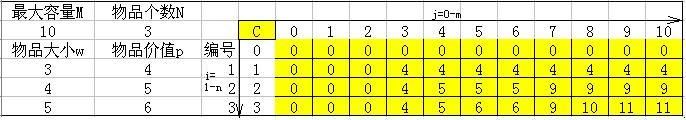
\includegraphics[width=360pt]{01knapsack.gif}\\
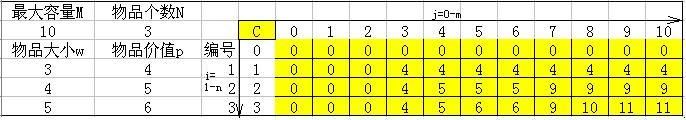
\includegraphics[width=0.5\textwidth]{01knapsack.png}\\
\figcaption{0-1背包问题的计算顺序}\label{fig:01knapsack}
\end{center}

当内循环是逆序时,且动规是用自底向上方式实现时,就可以保证同一行可以从右向左更新。

设一维数组为d(又称为滚动数组\footnote{刘汝佳,算法竞赛入门经典,清华大学出版社,2009,第169页9.3.3节}),
在更新d[j]之前,d[j]里保存的f[i-1][j],更新之后,d[j]里保存的是f[i][j]。

事实上,使用一维数组解0-1背包问题的程序在后面会被多次用到,所以这里抽象出一
个处理单个物品的函数,以后的代码中直接调用不加说明。
\begin{Code}
def ZeroOneKnapsack(d[], i)
    for j = W..w[i]
        d[j] = max(d[j], d[j-w[i]] + v[i])
\end{Code}

有了这个函数以后,0-1背包问题的伪代码就可以这样写:
\begin{Code}
d[0..W] = 0
for i = 1..N
    ZeroOneKnapsack(d[], i)
\end{Code}

\subsubsection{代码}
版本1,自底向上。

\begin{Codex}[label=01knapsack.c]
#include <stdio.h>
#include <string.h>

#define MAXN 1000
#define MAXW 1000

int N, W;
int w[MAXN+1], v[MAXN+1]; /* 0 没有用 */

int f[MAXN + 1][MAXW + 1];

void dp() {
    int i, j;
    memset(f, 0, sizeof(f)); /* 背包不一定要装满 */
    for(i = 1; i <= N; ++i) {
        /* for(j = W; j >= 0; --j) { /* 也可以 */
        for(j = 0; j <= W; ++j) {
            f[i][j] = f[i-1][j];
            if(j >= w[i]) {
                const int tmp = f[i-1][j-w[i]] + v[i];
                if(tmp > f[i][j]) f[i][j] = tmp;
            }
        }
    }
}

int main() {
    int i, T;
    scanf("%d", &T);
    while(T--) {
        scanf("%d %d", &N, &W);
        for(i = 1; i <= N; ++i) scanf("%d", &v[i]);
        for(i = 1; i <= N; ++i) scanf("%d", &w[i]);

        dp();
        printf("%d\n", f[N][W]);
    }
    return 0;
}
\end{Codex}

版本2,自底向上,滚动数组。

\begin{Codex}[label=01knapsack2.c]
#include <stdio.h>
#include <string.h>

#define MAXN 1000
#define MAXW 1000

int N, W;
int w[MAXN], v[MAXN];

int d[MAXW + 1]; /* 滚动数组 */

/**
 * @brief 0-1背包问题中,处理单个物品.
 * @param[in] d 滚动数组
 * @param[in] i 该物品的下标
 * @return 无
 */
void zero_one_knapsack(int d[], const int i) {
    int j;
    for(j = W; j >= w[i]; --j) {
        const int tmp = d[j - w[i]] + v[i];
        if(tmp > d[j]) d[j] = tmp; /* 求最小用 <,求最大用 > */
    }
}

void dp() {
    int i;
    memset(d, 0, sizeof(d)); /* 背包不一定要装满 */

    for(i = 0; i < N; ++i) zero_one_knapsack(d, i);
}

int main() {
    int i, T;
    scanf("%d", &T);
    while(T--) {
        scanf("%d %d", &N, &W);
        for(i = 0; i < N; ++i) scanf("%d", &v[i]);
        for(i = 0; i < N; ++i) scanf("%d", &w[i]);

        dp();
        printf("%d\n", d[W]);
    }
    return 0;
}
\end{Codex}

\subsubsection{相关的题目}
与本题相同的题目:
\begindot
\item 《算法竞赛入门经典》\footnote{刘汝佳,算法竞赛入门经典,清华大学出版社,2009}第167页例题9-5
\item  HDOJ 2602 Bone Collector, \myurl{http://acm.hdu.edu.cn/showproblem.php?pid=2602}
\myenddot

与本题相似的题目:
\begindot
\item  wikioi 1014 装箱问题, \myurl{http://www.wikioi.com/problem/1014/}, \\
参考代码 \myurl{https://gist.github.com/soulmachine/6248518}
\myenddot

\subsection{完全背包问题}
\label{sec:ukp}

\subsubsection{描述}
给你一个储钱罐(piggy bank),往里面存硬币。存入的过程是不可逆的,要想把钱拿出来只能摔碎
储钱罐。因此,你想知道里面是否有足够多的钱,把它摔碎是值得的。

你可以通过储钱罐的重量来推测里面至少有多少钱。已知储钱罐空的时候的重量和装了硬币后的重量,
还有每种硬币的重量和面值,每种硬币的数量不限。求在最坏情况下,储钱罐里最少有多少钱。

\subsubsection{输入}
第1行包含一个整数T,表示有T组测试用例。
每组测试用例,第一行是两个整数E和F,分别表示空储钱罐的重量和装了硬币后的重量,以克(gram)为单位,
储钱罐的重量不会超过10kg,即$1 \leq E \leq F \leq 10000$。第二行是一个整数$N(1 \leq N \leq 500)$,表示
硬币的种类数目。接下来是N行,每行包含两个整数v和w($1 \leq v \leq 50000, 1 \leq w \leq 10000$),分别
表示硬币的面值和重量。

\subsubsection{输出}
每个案例打印一行。内容是"The minimum amount of money in the piggy-bank is X.",其中
X表示储钱罐里最少有多少钱。如果不能精确地达到给定的重量,则打印"This is impossible."。

\subsubsection{样例输入}
\begin{Code}
3
10 110
2
1 1
30 50
10 110
2
1 1
50 30
1 6
2
10 3
20 4
\end{Code}

\subsubsection{样例输出}
\begin{Code}
The minimum amount of money in the piggy-bank is 60.
The minimum amount of money in the piggy-bank is 100.
This is impossible.
\end{Code}

\subsubsection{分析}
每种物品有无限个可用,这是完全背包问题。

本题没有给出储钱罐的容量,但每个案例给出了,初始为空时的重量E和装了硬币后的重量F,
因此可以把储钱罐看作一个容量为F-E的背包,背包必须要装满。

这个问题非常类似于0-1背包问题,所不同的是每种物品有无限个。也就是从每种
物品的角度考虑,与它相关的策略已并非取或不取两种,而是取0个、取1个、取2
个……直至取$W/w[i]$个。

一种好想好写的基本方法是转化为0-1背包问题:把第i种物品换成$W/w[i]$个0-1
背包问题中的物品,则得到了物品数为$\sum \dfrac{W}{w[i]}$的0-1背包问题。
时间复杂度是$O(W\sum \dfrac{W}{w[i]})$。

按照该思路,状态转移方程为:
$$f[i][j]=\max\left\{f[i-1][j-k*w[i]]+k*v[i], 0 \leq k*w[i] \leq j\right\}$$

伪代码如下:
\begin{Code}
for i = 1..N
    for j = W..w[i]
        for k = 1..j/w[i]
            d[j] = max{d[j], d[j-k*w[i]] + k*v[i]};
\end{Code}

也可以写成:
\begin{Code}
for i = 1..N
    for k = 1..W/w[i]
        ZeroOneKnapsack(d[], w, v)
\end{Code}

“拆分物品”还有更高效的拆分方法:把第i种物品拆分成重量为$2^k*w[i]$、价值为$2^k*v[i]$的
若干物品,其中k取所有满足$2^k*w[i] \leq W$的非负整数。这是二进制的思想,因为闭区间[1, W/w[i]]中
的任何整数都可以表示为$1, 2, 4, ..., 2^k$中若干个的和。

这样处理单个物品的复杂度由$O\left(\dfrac{W}{w[i]}\right)$降到了$O\left(\log \dfrac{W}{w[i]}\right)$,伪代码如下:
\begin{Code}
def UnboundedKnapsack(d[], i)
    k=1
    while k*w[i] <= W
        ZeroOneKnapsack(d[], k*w[i], k*v[i])
        k=2*k
\end{Code}

还存在更优化的算法,复杂度为$O(NW)$,伪代码如下:
\begin{Code}
for i = 1..N
    for j = 0..W
        d[j] = max{d[j], d[j-w[i]] + v[i]};
\end{Code}

与0-1背包问题相比,仅有一行代码不同,这里内循环是顺序的,而0-1背包是逆序的(在使用滚动数组的情况下)。

为什么这个算法可行呢?首先想想为什么0-1背包中内循环要逆序,逆序是为了保证每个物品只选一次,保证在
“选择第i件物品”时,依赖的是一个没有选择第i件物品的子结果$f[i-1][j-w[i]]$。而现在完全背
包的特点却是每种物品可选无限个,没有了每个物品只选一次的限制,所以就可以并且必须采用j递增
的顺序循环。

根据上面的伪代码,状态转移方程也可以写成这种形式:
$$f[i][j]=\max\left\{f[i-1][j], f[i][j-w[i]+v[i]\right\}$$

抽象出处理单个物品的函数:
\begin{Code}
def UnboundedKnapsack(d[], i)
    for j = w[i]..W
        d[j] = max(d[j], d[j-w[i]] + v[i])
\end{Code}

\subsubsection{代码}
\begin{Codex}[label=piggy_bank.c]
#include <stdio.h>

#define MAXN 500
#define MAXW 10000
 /* 无效值,不要用0x7FFFFFFF,执行加运算后会变成负数 */
const int INF = 0x0FFFFFFF;

int N, W;
int w[MAXN], v[MAXN];

int d[MAXW + 1]; /* 滚动数组 */

/**
 * @brief 完全背包问题中,处理单个物品.
 * @param[in] d 滚动数组
 * @param[in] i 该物品的下标
 * @return 无
 */
void unbounded_knapsack(int d[], const int i) {
    int j;
    for(j = w[i]; j <= W; ++j) {
        const int tmp = d[j - w[i]] + v[i];
        if(tmp < d[j]) d[j] = tmp; /* 求最小用 <,求最大用 > */
    }
}
/** c,物品的系数 */
void zero_one_knapsack(int d[], const int i, const int c) {
    int j;
    const int neww = c * w[i];
    const int newv = c * v[i];
    for(j = W; j >= neww; --j) {
        const int tmp = d[j - neww] + newv;
        if(tmp < d[j]) d[j] = tmp;  /* 求最小用 <,求最大用 > */
    }
}

void unbounded_knapsack1(int d[], const int i) {
    int k = 1;
    while(k * w[i] <= W) {
        zero_one_knapsack(d, i, k);
        k *= 2;
    }
}

void dp() {
    int i;
    for(i = 0; i <= W; ++i) d[i] = INF; /* 背包要装满 */
    d[0] = 0;

    for(i = 0; i < N; ++i) unbounded_knapsack(d, i);
}

int main() {    
    int i, T;
    int E, F;
 
    scanf("%d", &T);
    while(T--) {
        scanf("%d %d", &E, &F);
        W = F - E;
        scanf("%d", &N);
        for(i = 0; i < N; ++i) scanf("%d %d", &v[i], &w[i]);

        dp();
        if(d[W] == INF) {
            printf("This is impossible.\n");
        } else {
            printf("The minimum amount of money in the piggy-bank is %d.\n",
                    d[W]);
        }
    }
    return 0;
}

/* 将第i种物品取0个,1个,...,W/w[i]个,该版本不能AC,会TLE */
void unbounded_knapsack2(int d[], const int w, const int v) {
    int j, k;
    for(j = W; j >= w; --j) {
        const int K = j / w;
        for(k = 1; k <= K; ++k) {
            const int tmp = d[j - k * w] + k * v;
            if(tmp < d[j]) d[j] = tmp; /* 求最小用 <,求最大用 > */
        }
    }
}

/* 将第i种物品取0个,1个,...,W/w[i]个,该版本不能AC,会TLE */
void unbounded_knapsack3(int d[], const int w, const int v) {
    int k;
    const int K = W / w;
    for(k = 0; k < K; ++k){
        zero_one_knapsack(d, w, v);
    }
}
\end{Codex}

\subsubsection{相关的题目}
与本题相同的题目:
\begindot
\item 《算法竞赛入门经典》\footnote{刘汝佳,算法竞赛入门经典,清华大学出版社,2009}第167页例题9-4
\item POJ 1384 Piggy-Bank, \myurl{http://poj.org/problem?id=1384}
\item HDOJ 1114 Piggy-Bank, \myurl{http://t.cn/zWXbXIn}
\myenddot

与本题相似的题目:
\begindot
\item POJ 2063 Investment, \myurl{http://poj.org/problem?id=2063}
\myenddot

\subsection{多重背包问题}

\subsubsection{描述}
某地发生地震,为了挽救灾区同胞的生命,心系灾区同胞的你准备自己采购一些粮食
支援灾区,现在假设你一共有资金W元,而市场有N种大米,每种大米都是袋装产品,
其价格不等,并且只能整袋购买。

请问:你用有限的资金最多能采购多少公斤粮食呢?

\subsubsection{输入}
第1行包含一个整数T,表示有T组测试用例。
每组测试用例的第一行是两个整数W和N($1 \leq W \leq 100, 1 \leq N \leq 100$),分别表示经费的金
额和大米的种类,然后是N行数据,每行包含3个整数w,v和c
($1 \leq w \leq 20,1 \leq v \leq 200,1 \leq c \leq 20$),
分别表示每袋的价格、每袋的重量以及对应种类大米的袋数。

\subsubsection{输出}
对于每组测试用例,输出能够购买大米的最大重量,你可以假设经费买不光所有的大米,
并且经费你可以不用完。每个实例的输出占一行。

\subsubsection{样例输入}
\begin{Code}
1
8 2
2 100 4
4 100 2
\end{Code}

\subsubsection{样例输出}
\begin{Code}
400
\end{Code}

\subsubsection{分析}
第i种物品有c[i]个可用,这是多重背包问题。

与完全背包问题类似,也可以用“拆分物品”的思想把本问题转化为0-1背包问题:把
第i种物品换成$c[i]$个0-1背包问题中的物品,则得到了物品数为$\sum c[i]$的0-1背包问题。
时间复杂度是$O(W\sum c[i])$。状态转移方程为:
$$f[i][j]=\max\left\{f[i-1][j-k*w[i]]+k*v[i], 0 \leq k \leq c[i], 0 \leq k*w[i] \leq j\right\}$$

伪代码如下:
\begin{Code}
for i = 1..N
    for j = W..w[i]
        K = min{j/w[i], c[i]}
        for k = 1..K
            d[j] = max{d[j], d[j-k*w[i]] + k*v[i]};
\end{Code}

也可以写成:
\begin{Code}
for i = 1..N
    for k = 1..c[i]
        ZeroOneKnapsack(d[], i)
\end{Code}

拆分物品也可以使用二进制的技巧,把第i种物品拆分成若干物品,其中每件物品都有一个
系数,这个新物品的重量和价值均是原来的重量和价值乘以这个系数。系数分别为
$1,2,2^2,...,2^{k-1},c[i]-2^k+1$,其中k是满足$2^k-1<c[i]$的最大整数。例如,某种物品
有13个,即c[i]=13,则相应的k=3,这种物品应该被拆分成系数分别1,2,4,6的四个物品。

这样处理单个物品的复杂度由$O(c[i])$降到了$O(\log c[i])$,伪代码如下:
\begin{Code}
// c, 物品系数
def ZeroOneKnapsack(d[], i, c)
    for j = W..w[i]
        d[j] = max(d[j], d[j-c*w[i]] + c*v[i])
def BoundedKnapsack(d[], i)
    if c[i]*w[i] >= W
        unbounded_knapsack(d[], i);
        return;

    k = 1;
    while k < c[i]
        zero_one_knapsack(d[], i, k);
        c[i] -= k;
        k *= 2;

    zero_one_knapsack(d[], i, c);
\end{Code}

\subsubsection{代码}
\begin{Codex}[label=bkp.c]
#include <stdio.h>
#include <string.h>

#define MAXN 100
#define MAXW 100

int N, W;
int w[MAXN], v[MAXN], c[MAXN];

int d[MAXW + 1]; /* 滚动数组 */

/** c,物品的系数 */
void zero_one_knapsack(int d[], const int i, const int c) {
    int j;
    const int neww = c * w[i];
    const int newv = c * v[i];
    for(j = W; j >= neww; --j) {
        const int tmp = d[j - neww] + newv;
        if(tmp > d[j]) d[j] = tmp;  /* 求最小用 <,求最大用 > */
    }
}

void unbounded_knapsack(int d[], const int i) {
    int j;
    for(j = w[i]; j <= W; ++j) {
        const int tmp = d[j - w[i]] + v[i];
        if(tmp > d[j]) d[j] = tmp; /* 求最小用 <,求最大用 > */
    }
}

/**
 * @brief 多重背包问题中,处理单个物品.
 * @param[in] d 滚动数组
 * @param[in] i 该物品的下标
 * @param[in] c 该物品的数量
 * @return 无
 */
void bounded_knapsack(int d[], const int i) {
    int k;
    for(k = 0; k < c[i]; ++k) {
        zero_one_knapsack(d, i, 1);
    }
}

/* 另一个版本,拆分物品更加优化 */
void bounded_knapsack1(int d[], const int i) {
    int k;
    if(c[i] * w[i] >= W) {
        unbounded_knapsack(d, i);
        return;
    }

    k = 1;
    while(k < c[i]) {
        zero_one_knapsack(d, i, k);
        c[i] -= k;
        k *= 2;
    }
    zero_one_knapsack(d, i, c[i]);
}

void dp() {
    int i;
    memset(d, 0, sizeof(d)); /* 背包不一定要装满 */

    for(i = 0; i < N; ++i) bounded_knapsack1(d, i);
}
 
int main() {
    int i;
    int T;
    scanf("%d", &T);
    while(T--) {
        scanf("%d %d", &W, &N);
        for(i = 0; i < N; ++i) scanf("%d %d %d", &w[i], &v[i], &c[i]);

        dp();
        printf("%d\n", d[W]);
    }
    return 0;
}
\end{Codex}

\subsubsection{相关的题目}
与本题相同的题目:
\begindot
\item HDOJ 2191 买大米, \myurl{http://acm.hdu.edu.cn/showproblem.php?pid=2191}
\myenddot

与本题相似的题目:
\begindot
\item None
\myenddot


\section{序列型动态规划} %%%%%%%%%%%%%%%%%%%%%%%%%%%%%%
对于所有动规题目,如果把状态转移图画出来,一定是一个有向无环图(DAG)。再进一步细分类别,有序列型动态规划,棋盘型动态规划,树型动态规划等等。


\subsection{最长上升子序列}

\subsubsection{描述}
当一个序列严格递增时,我们称这个序列是上升的。
对于一个给定的序列$(a_1, a_2, ..., a_N)$,我们可以得到一些上升的子序列$(a_{i1}, a_{i2}, ..., a_{iK})$,
这里$1 \leq i1 < i2 < ... < iK \leq N$。例如,对于序列(1, 7, 3, 5, 9, 4, 8),
有它的一些上升子序列,如(1, 7), (3, 4, 8)等等,这些子序列中最长的长度是4,比如子序列(1, 3, 5, 8)。

对于给定的序列,求\textbf{最长上升子序列}(longest increasing subsequence)的长度。

\subsubsection{输入}
第一行是序列的长度$N (1 \leq N \leq 1000)$。
第二行给出序列中的N个整数,这些整数的取值范围都在0到10000。

\subsubsection{输出}
最长上升子序列的长度。

\subsubsection{样例输入}
\begin{Code}
7
1 7 3 5 9 4 8
\end{Code}

\subsubsection{样例输出}
\begin{Code}
4
\end{Code}

\subsubsection{分析}
设状态为d[j],表示以$a_j$为终点的最长上升子序列的长度。状态转移方程如下;
$$
d[j]=\begin{cases}
1 & j=1\\
\max\left\{d[i]\right\}+1 & 1<i<j,a_i<a_j
\end{cases}
$$

\subsubsection{代码}

\begin{Codex}[label=lis.c]
#include<stdio.h>
#define MAXN 1001 // a[0]未用

int N;
int a[MAXN];
int d[MAXN];

void dp() {
    int i, j;
    d[1] = 1;
 
    for (j = 2; j <= N; j++) { // 每次求以aj为终点的最长上升子序列的长度
        int max = 0;  // 记录aj左边的上升子序列的最大长度 
        for (i = 1; i < j; i++)  if (a[i] <a[j] && max < d[i]) max = d[i];
        d[j] = max + 1;
    }
}

int main() {
    int i, max;
    scanf("%d",&N);
    for (i = 1; i <= N;i++) scanf("%d",&a[i]);
    
    dp();

    max = 0;
    for(i = 1; i <= N;i++) if (d[i] > max) max = d[i];
    printf("%d\n",max);
    return 0;
}
\end{Codex}

\subsubsection{相关的题目}
与本题相同的题目:
\begindot
\item 《程序设计导引及在线实践》\footnote{李文新,程序设计导引及在线实践,清华大学出版社,2007}第198页例题10.3
\item 百练 2757 最长上升子序列, \myurl{http://poj.grids.cn/practice/2757/}
\item POJ 2533 Longest Ordered Subsequence, \myurl{http://poj.org/problem?id=2533}
\item wikioi 1576, 最长严格上升子序列, \myurl{http://www.wikioi.com/problem/1576/}
\myenddot

与本题相似的题目:
\begindot
\item  wikioi 1044 拦截导弹,\myurl{http://www.wikioi.com/problem/1044/}, \\
参考代码 \myurl{https://gist.github.com/soulmachine/6248489}
\myenddot


\subsection{嵌套矩形}

\subsubsection{描述}
有$n$个矩形,每个矩形可以用$a,b$来描述,表示长和宽。矩形$X(a,b)$可以嵌套在
矩形$Y(c,d)$中当且仅当$a<c,b<d$或者$b<c,a<d$(相当于旋转X90度)。例如
(1,5)可以嵌套在(6,2)内,但不能嵌套在(3,4)中。你的任务是选出尽可能多的
矩形排成一行,使得除最后一个外,每一个矩形都可以嵌套在下一个矩形内。

\subsubsection{输入}
第一行是一个正整数$N(0<N<10)$,表示测试数据组数,
每组测试数据的第一行是一个正正数n,表示该组测试数据中含有矩形的个数$(n<=1000)$
随后的n行,每行有两个数$a,b(0<a,b<100)$,表示矩形的长和宽

\subsubsection{输出}
每组测试数据都输出一个数,表示最多符合条件的矩形数目,每组输出占一行

\subsubsection{样例输入}
\begin{Code}
1
10
1 2
2 4
5 8
6 10
7 9
3 1
5 8
12 10
9 7
2 2
\end{Code}

\subsubsection{样例输出}
\begin{Code}
5
\end{Code}

\subsubsection{分析}
本题实质上是求DAG中不固定起点的最长路径。

设d[i]表示从结点i出发的最长长度,状态转移方程如下:
$$d[i]=\max\left\{d[j]+1|(i,j) \in E\right\}$$

其中,E为边的集合。最终答案是d[i]中的最大值。

\subsubsection{代码}
\begin{Codex}[label=embedded_rectangles.c]
#include <stdio.h>
#include <string.h>

#define MAXN 1000 // 矩形最大个数

int n; // 矩形个数
int G[MAXN][MAXN]; // 矩形包含关系
int d[MAXN]; // 表格

/**
 * @brief 备忘录法.
 * @param[in] i 起点
 * @return 以i为起点,能达到的最长路径
 */
int dp(const int i) {
    int j;
    int *ans= &d[i];
    if(*ans > 0) return *ans;

    *ans = 1;
    for(j = 0; j < n; j++) if(G[i][j]) {
        const int next = dp(j) + 1;
        if(*ans < next) *ans = next;
    }
    return *ans;
}

/**
 * @brief 按字典序打印路径.
 *
 * 如果多个 d[i] 相等,选择最小的i。
 *
 * @param[in] i 起点
 * @return 无
 */
void print_path(const int i) {
    int j;
    printf("%d ", i);
    for(j = 0; j < n; j++) if(G[i][j] && d[i] == d[j] + 1) {
        print_path(j);
        break;
    }
}

int main() {
    int N, i, j;
    int max, maxi;
    int a[MAXN],b[MAXN];

    scanf("%d", &N);
    while(N--) {
        memset(G, 0, sizeof(G));
        memset(d, 0, sizeof(d));

        scanf("%d", &n);
        for(i = 0; i < n; i++) scanf("%d%d", &a[i], &b[i]);

        for(i = 0; i < n; i++)
            for(j = 0; j < n; j++)
                if((a[i] > a[j] && b[i] > b[j]) ||
                    (a[i] > b[j] && b[i] > a[j])) G[i][j] = 1;

        max = 0;
        maxi = -1;
        for(i = 0; i < n; i++) if(dp(i) > max) {
            max = dp(i);
            maxi = i;
        }
        printf("%d\n", max);
        // print_path(maxi);
    }
    return 0;
}
\end{Codex}

\subsubsection{相关的题目}
与本题相同的题目:
\begindot
\item 《算法竞赛入门经典》\footnote{刘汝佳,算法竞赛入门经典,清华大学出版社,2009}第161页9.2.1节
\item  NYOJ 16 嵌套矩形, \myurl{http://acm.nyist.net/JudgeOnline/problem.php?pid=16}
\myenddot

与本题相似的题目:
\begindot
\item  None
\myenddot


\subsection{线段覆盖 2}

\subsubsection{描述}
数轴上有$n(n \leq 1000)$条线段,线段的两端都是整数坐标,坐标范围在$0 \sim 1000000$,每条线段有一个价值,请从$n$条线段中挑出若干条线段,使得这些线段两两不覆盖(端点可以重合)且线段价值之和最大。

\subsubsection{输入}
第一行一个整数$n$,表示有多少条线段。

接下来$n$行每行三个整数, $a_i,b_i,c_i$,分别代表第$i$条线段的左端点$a_i$,右端点$b_i$(保证左端点<右端点)和价值$c_i$。

\subsubsection{输出}
输出能够获得的最大价值

\subsubsection{样例输入}
\begin{Code}
3
1 2 1
2 3 2
1 3 4
\end{Code}

\subsubsection{样例输出}
\begin{Code}
4
\end{Code}

\subsubsection{分析}
先将线段排序。按照右端点从小到大排序。原因是循环结构中是$i$从$1$到$n$, $i$比较小的时候尽可能选右端点比较小的,这样才可以为后面的线段留下更大的空间。

设状态为f[i],表示前i条线段时,选上第i条线段,能获得的最大价值。状态转移方程如下:
$$
f[i]=\max\left\{f[j]\right\}+c[i], 2 \leq i \leq n, 1 \leq j \leq i-1,\text{且b[j]<=a[i]}
$$
b[j]<=a[i]表示j的右端点在i的左端点左边,即不重合。

输出f[i]数组中的最大值。

\subsubsection{代码}

\begin{Codex}[label=lines_cover.c]
/* http://www.wikioi.com/problem/3027/ */
#include <stdio.h>
#include <stdlib.h>
#include <limits.h>

#define MAXN 1000

typedef struct line_t {
    int a, b, c;
} line_t;

int line_cmp(const void *a, const void *b) {
    line_t *la = (line_t*)a;
    line_t *lb = (line_t*)b;
    return la->b - lb->b;
}

int n;
line_t line[MAXN];
int f[MAXN];

void dp() {
    int i, j;
    qsort(line, n, sizeof(line_t), line_cmp);
    f[0] = line[0].c;

    for (i = 1; i < n; i++) {
        int max = 0;
        for (j = 0; j < i; j++) {
            if (line[j].b <= line[i].a) max = max > f[j] ? max : f[j];
        }
        f[i] = max + line[i].c;
    }
}


static int max_element(const int a[], int begin, int end) {
    int i;
    int max_value = INT_MIN;
    int max_pos = -1;
    for (i = begin; i < end; i++) {
        if (max_value < a[i]) {
            max_value = a[i];
            max_pos = i;
        }
    }
    return max_pos;
}


int main() {
    int i;
    scanf("%d", &n);
    for (i = 0; i < n; i++) scanf("%d%d%d", &line[i].a, &line[i].b, &line[i].c);

    dp();

    printf("%d\n", f[max_element(f, 0, n)]);
    return 0;
}
\end{Codex}

\subsubsection{相关的题目}
与本题相同的题目:
\begindot
\item  wikioi 3027 线段覆盖 2, \myurl{http://www.wikioi.com/problem/3027/}
\myenddot

与本题相似的题目:
\begindot
\item  None
\myenddot


\subsection{硬币问题}

\subsubsection{描述}
有$n$种硬币,面值为别为$v_1,v_2,v_3,\cdots, v_n$,每种都有无限多。给定非负整数$S$,可以
选取多少个硬币,使得面值和恰好为$S$?输出硬币数目的最小值和最大值。
$1 \leq n \leq 100, 1 \leq S \leq 10000, 1 \leq v_i \leq S$。

\subsubsection{输入}
第1行$n$,
第2行$S$,
第3到$n+2$行为$n$种不同的面值。

\subsubsection{输出}
第1行为最小值,
第2行为最大值。

\subsubsection{样例输入}
\begin{Code}
3
6
1
2
3
\end{Code}

\subsubsection{样例输出}
\begin{Code}
2
6
\end{Code}

\subsubsection{分析}
本题实质上是求DAG中固定终点的最长路径和最短路径。

把每种面值看作一个点,表示“还需要凑足的面值”,则初始状态为S,目标状态为0。若当前状态为i,
每使用一个硬币j,状态便转移到$i-v_j$。

设状态为d[i],表示从节点i出发的最长路径长度,则原问题的解是d[S]。状态转移方程如下:
$$d[i]=\max\left\{d[j]+1,(i,j) \in E\right\}$$

本题还可以看作是完全背包问题(见\S \ref{sec:ukp}节):背包容量为S,背包必须要装满,物品即硬币,每个硬币的费用为面值$v_i$,
价值均为1。求背包中物品的最小价值和最大价值。

\subsubsection{代码}
版本1,备忘录法。

\begin{Codex}[label=coin_change.c]
#include<stdio.h>
#include <string.h>

#define MAXN 100
#define MAXV 10000

/** 硬币面值的种类. */
int n;
/** 要找零的数目. */
int S;
/** 硬币的各种面值. */
int v[MAXN];
/** min[i] 表示面值之和为i的最短路径的长度,max则是最长. */
int min[MAXV + 1], max[MAXV + 1];

/**
 * @brief 最短路径.
 * @param[in] s 面值
 * @return 最短路径长度
 */
int dp1(const int s) { // 最小值
    int i;
    int *ans = &min[s];
    if(*ans != -1) return *ans;
    *ans = 1<<30;
    for(i = 0; i < n; ++i) if(v[i] <= s) {
        const int tmp = dp1(s-v[i])+1;
        *ans = *ans < tmp ? *ans : tmp;
    }
    return *ans;
}

int visited[MAXV + 1];
/**
 * @brief 最长路径.
 * @param[in] s 面值
 * @return 最长路径长度
 */
int dp2(const int s) { //最大值 
    int i;
    int *ans = &max[s];

    if(visited[s]) return max[s];
    visited[s] = 1;

    *ans = -1<<30;
    for(i = 0; i < n; ++i) if(v[i] <= s) {
        const int tmp = dp2(s-v[i])+1;
        *ans = *ans > tmp ? *ans : tmp;
    }
    return *ans;
}

void print_path(const int* d, const int s);

int main() {
    int i;
    scanf("%d%d", &n, &S);
    for(i = 0; i < n; ++i) scanf("%d", &v[i]);

    memset(min, -1, sizeof(min));
    min[0] = 0;
    printf("%d\n", dp1(S));
    // print_path(min, S);

    memset(max, -1, sizeof(max));
    memset(visited, 0, sizeof(visited));
    max[0] = 0; visited[0] = 1;
    printf("%d\n", dp2(S));
    // print_path(max, S);

    return 0;
}

/**
 * @brief 打印路径.
 * @param[in] d 上面的 min 或 min
 * @param[in] s 面值之和
 * @return 无
 */
void print_path(const int* d, const int s) {//打印的是边
    int i;
    for(i = 0; i < n; ++i) if(v[i] <= s && d[s-v[i]] + 1 == d[s]) {
        printf("%d ",i);
        print_path(d, s-v[i]);
        break;
    }
    printf("\n");
}
\end{Codex}

版本2,自底向上。

\begin{Codex}[label=coin_change2.c]
#include<stdio.h>

#define MAXN 100
#define MAXV 10000

int n, S, v[MAXN], min[MAXV + 1], max[MAXV + 1];
int min_path[MAXV], max_path[MAXV];

void dp() {
    int i, j;

    min[0] = max[0] = 0;
    for(i = 1; i <= S; ++i) {
        min[i] = MAXV; 
        max[i] = -MAXV;
    }

    for(i = 1; i <= S; ++i) {
        for(j = 0; j < n; ++j) if(v[j] <= i) {
            if(min[i-v[j]] + 1 < min[i]) {
                min[i] = min[i-v[j]] + 1;
                min_path[i] = j;
            }
            if(max[i-v[j]] + 1 > max[i]) {
                max[i] = max[i-v[j]] + 1;
                max_path[i] = j;
            }
        }
    }
}

void print_path(const int *d, int s);

int main() {
    int i;
    scanf("%d%d", &n, &S);
    for(i = 0; i < n; ++i) scanf("%d", &v[i]);

    dp();
    printf("%d\n", min[S]);
    // print_path(min_path, S);
    printf("%d\n", max[S]);
    // print_path(max_path, S);
    return 0;
}

/**
 * @brief 打印路径.
 * @param[in] d 上面的 min_path 或 min_path
 * @param[in] s 面值之和
 * @return 无
 */
void print_path(const int *d, int s) {
    while(s) {
        printf("%d ", d[S]);
        S -= v[d[s]];
    }
    printf("\n");
}
\end{Codex}

版本3,当作完全背包问题。

\begin{Codex}[label=coin_change3.c]
#include <stdio.h>
#include <string.h>

#define MAXN 100
#define MAXW 10000
 /* 无效值,不要用0x7FFFFFFF,执行加运算后会变成负数 */
const int INF = 0x0FFFFFFF;

int N, W;
int w[MAXN], v[MAXN];

int min[MAXW + 1], max[MAXW + 1]; /* 滚动数组 */

int min_path[MAXW + 1], max_path[MAXW + 1];
void print_path(const int *d, int s);

/**
 * @brief 完全背包问题中,处理单个物品.
 * @param[in] d 滚动数组
 * @param[in] i 该物品的下标
 * @return 无
 */
void unbounded_knapsack(int min[], int max[], const int i) {
    int j;
    for(j = w[i]; j <= W; ++j) {
        if(min[j - w[i]] + v[i] < min[j]) {
            min[j] = min[j - w[i]] + v[i];
            // min_path[j] = i;
        }
        if(max[j - w[i]] + v[i] > max[j]) {
            max[j] = max[j - w[i]] + v[i];
            // max_path[j] = i;
        }
    }
}

void dp() {
    int i, j;
    min[0] = 0;
    max[0] = 0;
    for(j = 1; j <= W; ++j) { /* 背包要装满 */
        min[j] = INF;
        max[j] = -INF;
    }

    for(i = 0; i < N; ++i) unbounded_knapsack(min, max, i);
}

int main() {
    int i;
    for (i = 0; i < MAXN; ++i) v[i] = 1;
    scanf("%d%d", &N, &W);
    for(i = 0; i < N; ++i) scanf("%d", &w[i]);

    dp();
    printf("%d\n", min[W]);
    // print_path(min_path, W);
    printf("%d\n", max[W]);
    // print_path(max_path, W);
    return 0;
}

/**
 * @brief 打印路径.
 * @param[in] d 上面的 min_path 或 min_path
 * @param[in] j 面值之和
 * @return 无
 */
void print_path(const int *d, int j) {
    while(j) {
        printf("%d ", d[j]);
        j -= w[d[j]];
    }
    printf("\n");
}
\end{Codex}

\subsubsection{相关的题目}
与本题相同的题目:
\begindot
\item 《算法竞赛入门经典》\footnote{刘汝佳,算法竞赛入门经典,清华大学出版社,2009}第162页例题9-3
\item  tyvj 1214 硬币问题, \myurl{http://www.tyvj.cn/problem_show.aspx?id=1214}
\myenddot

与本题相似的题目:
\begindot
\item  None
\myenddot


\section{区间型动态规划} %%%%%%%%%%%%%%%%%%%%%%%%%%%%%%


\subsection{最优矩阵链乘}
\subsubsection{描述}
一个$m \times n$的矩阵乘以一个$n \times p$的矩阵等于一个$m \times p$的矩阵,运算量为$mnp$。

矩阵乘法不满足分配律,但满足结合律,即$A \times B \times C=(A \times B) \times C=A \times (B \times C)$。

假设A、B、C分别是$2 \times 3$、$3 \times 4$、$4 \times 5$的矩阵,则$(A \times B) \times C$的运算量为$2 \times 3 \times 4 + 2 \times 4 \times 5=64$,$A \times (B \times C)$的运算量为$3 \times 4 \times 5 + 2 \times 3 \times 5=90$,显然第一种运算顺序节省运算量。

给出N个矩阵组成的序列,设计一种方法把它们依次乘起来,使得总的运算量尽量小。

\subsubsection{输入}
对于每个矩阵序列,只给出它们的维度。每个序列由两个部分组成,第一行包含一个整数N,表示矩阵的个数;接下来的N行,每行一对整数,分别表示矩阵的行数和列数。给出的顺序与矩阵链乘的顺序一致。最后一行N为0,表示输入结束。N不大于10。

\subsubsection{输出}
假设矩阵命名为$A_1,A_2,...,A_N$。对每个测试用例输出一行,包含一个使用了小括号的表达式,清晰地指出乘法的先后顺序。每行输出以"Case x: "为前缀,x表示测试用例编号。如果有多个正确结果,只需要输出其中一个。

\subsubsection{样例输入}
\begin{Code}
3
1 5
5 20
20 1
3
5 10
10 20
20 35
6
30 35
35 15
15 5
5 10
10 20
20 25
0
\end{Code}

\subsubsection{样例输出}
\begin{Code}
Case 1: (A1 x (A2 x A3))
Case 2: ((A1 x A2) x A3)
Case 3: ((A1 x (A2 x A3)) x ((A4 x A5) x A6))
\end{Code}

\subsubsection{分析}
假设第i个矩阵$A_i$的维度是$p_{i-1} \times p_i$, i=1..N。

设状态为d[i][j],表示子问题$A_i, A_{i+1},..., A_j$的最优解,状态转移方程如下:
$$d[i][j]=\min\left\{d[i][k]+d[k+1][j] + p_{i-1}p_kp_j\right\}$$

\subsubsection{代码}
\begin{Codex}[label=oams.c]
#include <stdio.h>
#include <memory.h>
#include <limits.h>

#define INF INT_MAX
#define MAXN 10

int N;  /** 矩阵的个数. */
int p[MAXN + 1];  /** 矩阵Ai的维度是p[i-1]xp[i]. */
int d[MAXN][MAXN];  /** 状态,d[i][j]表示子问题Ai~Aj 的最优解. */
int s[MAXN][MAXN]; /** 子问题Ai~Aj 应该在s[i][j]处断开 */

/**
 * @brief 打印子问题Ai~Aj的解
 * @param[in] i Ai
 * @param[in] j Aj
 * @return 无
 */
void print(const int i, const int j) {
    if (i == j) {
        printf("A%d",i);
    } else {  /* i < j */
        printf("(");
        print(i, s[i][j]);
        printf(" x ");
        print(s[i][j]+1, j);
        printf(")");
    }
}

void dp() {
    int i, j, k, l; /* l表示区间长度 */
    for (i = 1;i <= N; ++i) d[i][i]=0;

    for (l = 2; l <= N; ++l) {
        for (i = 1; i <= N - l + 1; ++i) {
            j = i + l -1;
            d[i][j] = INF;
            for (k = i; k < j; ++k) {
                if (d[i][j] > d[i][k] + d[k+1][j] + p[i-1] * p[k] * p[j]) {
                    d[i][j] = d[i][k] + d[k+1][j] + p[i-1] * p[k] * p[j];
                    s[i][j] = k;
                }
            }
        }
    }
}

int main() {
    int i;
    int cas = 1;
    while (scanf("%d", &N) && N > 0) {
        memset(s, 0, sizeof(s));
        for (i = 0; i < N; ++i)  scanf("%d %d",&p[i],&p[i+1]);

        dp();

        printf("Case %d: ", cas++);
        print(1, N);
        printf("\n");
    }
    return 0;
}
\end{Codex}

\subsubsection{相关的题目}
与本题相同的题目:
\begindot
\item UVa 348 Optimal Array Multiplication Sequence, \myurl{http://t.cn/zH2pchp}
\item ZOJ 1276 Optimal Array Multiplication Sequence, \myurl{http://t.cn/zH2gW1P}
\myenddot

与本题相似的题目:
\begindot
\item wikioi 1154, 能量项链, \myurl{http://www.wikioi.com/problem/1154}, \\
参考代码 \myurl{https://gist.github.com/soulmachine/6248459}
\item Matrix67 - 十个利用矩阵乘法解决的经典题目,\myurl{http://www.matrix67.com/blog/archives/276}
\myenddot


\subsection{石子合并}
\subsubsection{描述}
在一条直线上摆着$N$堆石子。现要将石子有次序地合并成一堆。规定每次只能选相邻的2堆石子合并成新的一堆,并将新的一堆石子数记为该次合并的得分。

试设计一个算法,计算出将$N$堆石子合并成一堆的最小得分。

\subsubsection{输入}
第一行是一个数$N, 1 \leq N \leq 40000$,表示堆数。

接下来的N行每行一个数,表示该堆的石子数目。

\subsubsection{输出}
一个整数,即$N$堆石子合并成一堆的最小得分。

\subsubsection{样例输入}
\begin{Code}
4
1
1
1
1
\end{Code}

\subsubsection{样例输出}
\begin{Code}
8
\end{Code}

\subsubsection{分析}
这题与前面的矩阵链乘非常相似,只是计算代价的方式不同。设状态为$d(i,j)$,表示子问题第$i$堆到第$j$堆石子的最优解,状态转移方程如下:
$$d(i,j)=\min\left\{d(i,k)+d(k+1,j) + \text{sum}(i,j)\right\}$$
sum$(i,j)$表示从第$i$堆到第$j$堆的石子总数。代码见\myurl{https://gist.github.com/soulmachine/6195139}

上面的动规算法可以用四边形不等式进行优化,将时间复杂度从$O(N^3)$下降到$O(N^2)$。代码见\myurl{https://TODO}

无论如何,时间复杂度都是$O(N^2)$,本题中$N$范围特别大,开不了这么大的二维数组。所以动规算法只能处理小规模的情况。下面介绍第三种解法,Garsia-Wachs算法\footnote{Donald E. Knuth, The art of computer programming, volume 3, 2nd ed, p446}。

假设我们只对3堆石子a,b,c进行合并, 先合并哪两堆, 能使得得分最小?有两种方案:\\
score1 = (a+b) + ((a+b)+c)\\
score2 = (b+c) + ((b+c)+a)\\
假设score1 <= score2, 可以推导出 a <= c,反过来,只要a和c的关系确定,合并的顺序也确定。这就是\textbf{2-递减性质}。

Garsia-Wachs算法,就是基于这个性质,找出序列中满足A[i-1] <= A[i+1]最小的i,合并temp = A[i]+A[i-1],接着往前面找是否有满足A[j] > temp,把temp值插入A[j]的后面(数组的右边)。循环这个过程一直到只剩下一堆石子结束。

例如,\\
13 9 5 7 8 6 14\\
首先,找第一个满足A[i-1] <= A[i+1]的三个连续点,本例中就是 5 7 8,5和7合并得到12,12不是丢在原来的位置,而是将它插入到第一个比它大的元素的后面,得到\\
13 12 9 8 6 14

接着来,从左到右搜索三个连续点,找到 8 6 14,合并8和6的到14,将14插入到适当位置,得到 14 13 12 9 14

找到12 9 14,合并12和9得到21,将21插入到适当位置,得到21 14 13 14

找到 14 13 14,合并14 和 13 得到 27,将27插入到适当位置,得到27 21 14

因为27<14,先合并21和14,得到35,最后合并27和35,得到62,就是最终答案。

为什么要将temp插入A[j]的后面, 可以理解为是为了保持2-递减性质。从A[j+1]到A[i-2]看成一个整体 A[mid],现在A[j], A[mid], temp(A[i-1]+A[i]),因为temp < A[j],因此不管怎样都是A[mid]和temp先合并, 所以将temp值插入A[j]的后面不会影响结果。


\subsubsection{代码}
\begin{Codex}[label=stone_merge.c]
#include <stdio.h> 
#define MAXN 55555

int N, A[MAXN];  /* 堆数,每堆的石头个数 */
int num, result;  /* 数组实际长度,结果 */

void combine(int k) {  /* 前提 A[k-1] < A[k+1] */
    int i, j;

    /* 合并 k-1和k */
    int temp=A[k] + A[k-1];
    result += temp;
    /* 紧缩 */
    for(i = k; i < num - 1; i++) A[i] = A[i+1];
    num--;
    /* 插入temp到合适位置 */
    for(j = k-1; j > 0 && A[j-1] < temp; j--) A[j] = A[j-1];
    A[j] = temp;

    /* why? */
    while(j >= 2 && A[j] >= A[j-2]) {
        int d = num - j;
        combine(j - 1);
        j = num - d;
    }
}

int main() {
    int i;

    scanf("%d",&N);
    if(N == 0)    return 0;
    for(i = 0; i < N; i++) scanf("%d", &A[i]);

    num=2;
    result=0;
    for(i = 2; i < N; i++) {
        A[num++] = A[i];
        while(num >= 3 && A[num-3] <= A[num-1]) combine(num-2);
    }
    while(num > 1) combine(num-1);
    printf("%d\n",result);
    return 0;
}
\end{Codex}

\subsubsection{相关的题目}
与本题相同的题目:
\begindot
\item WIKIOI 1048 石子归并(数据规模很小), \myurl{http://www.wikioi.com/problem/1048/}
\item WIKIOI 2298 石子合并(数据规模很大), \myurl{http://www.wikioi.com/problem/2298/}
\item POJ 1738 An old Stone Game, \myurl{http://poj.org/problem?id=1738}
\myenddot

与本题相似的题目:
\begindot
\item None
\myenddot


\subsection{矩阵取数游戏}
\subsubsection{描述}
帅帅经常跟同学玩一个矩阵取数游戏:对于一个给定的$n*m$的矩阵,矩阵中的每个元素$a_{ij}$均为非负整数。游戏规则如下:
\begindot
\item 每次取数时须从每行各取走一个元素,共$n$个,$m$次后取完矩阵所有元素;
\item 每次取数时须从每行各取走一个元素,共$n$个,$m$次后取完矩阵所有元素;每次取走的各个元素只能是该元素所在行的行首或行尾;
\item 每次取数时须从每行各取走一个元素,共$n$个,$m$次后取完矩阵所有元素;每次取数都有一个得分值,为每行取数的得分之和,每行取数的得分= 被取走的元素值$*2i$,其中$i$表示第$i$次取数(从1开始编号);
\item 每次取数时须从每行各取走一个元素,共$n$个,$m$次后取完矩阵所有元素;游戏结束总得分为$m$次取数得分之和。
\myenddot

帅帅想请你帮忙写一个程序,对于任意矩阵,可以求出取数后的最大得分。

\subsubsection{输入}
第1行为两个用空格隔开的整数$n$和$m, 1 \leq n,m \leq 90$。
第$2 \sim n+1$ 行为$n*m$矩阵,其中每行有$m$个用单个空格隔开的非负整数$a_{ij}, 0 \leq a_{ij} \leq 1000$。

\subsubsection{输出}
输出仅包含1行,为一个整数,即输入矩阵取数后的最大得分。

\subsubsection{样例输入}
\begin{Code}
2 3
1 2 3
3 4 2
\end{Code}

\subsubsection{样例输出}
\begin{Code}
82
\end{Code}

\subsubsection{样例解释}
第1次:第1行取行首元素,第2行取行尾元素,本次得分为1*21+2*21=6

第2次:两行均取行首元素,本次得分为2*22+3*22=20

第3次:得分为3*23+4*23=56。总得分为6+20+56=82


\subsubsection{分析}
首先,每行之间是互相独立的,因此可以分别求出每行的最大得分,最后相加起来。

设状态为f(i,j),表示单行的区间[i,j]的最大值,转移方程为
$$
f(i,j) = \max\left\{f(i+1,j)+a(i)*2^x, f(i,j-1)+a(j)*2^x\right\}, 1 \leq x \leq m
$$
等价于
$$
f(i,j) = 2*\max\left\{f(i+1,j)+a(i), f(i,j-1)+a(j)\right\}
$$

同时,注意到,最大得分可能会非常大,因此需要用到大整数运算。预估一下最大得分,大概是 $1000*2^{80}$,用计算器算一下,有28位。

\subsubsection{代码}
\begin{Codex}[label=wikioi1166_matrix_game.c]
#include <stdio.h>
#include <memory.h>
#include <limits.h>

/* 一个数组元素表示4个十进制位,即数组是万进制的 */
#define BIGINT_RADIX 10000
#define RADIX_LEN 4
/* 1000*2^80 有 28 位 */
#define MAX_LEN (28/RADIX_LEN+1)  /* 整数的最大位数 */

/**
 * @brief 打印大整数.
 * @param[in] x 大整数,用数组表示,低位在低地址
 * @param[in] n 数组x的长度
 * @return 无
 */
void bigint_print(const int x[], const int n) {
    int i;
    int start_output = 0;  /* 用于跳过前导0 */
    for (i = n - 1; i >= 0; --i) {
        if (start_output) {  /* 如果多余的0已经都跳过,则输出 */
            printf("%04d", x[i]);
        } else if (x[i] > 0) {
            printf("%d", x[i]);
            start_output = 1; /* 碰到第一个非0的值,就说明多余的0已经都跳过 */
        }
    }

    if(!start_output) printf("0");  /* 当x全为0时 */
}

/**
 * @brief 一个32位整数转化为大整数bigint.
 * @param[in] n 32位整数
 * @param[out] x 大整数
 * @return 大整数
 */
int* int_to_bigint(int n, int x[]) {
    int i = 0;
    memset(x, 0, MAX_LEN * sizeof(int));
    while (n > 0) {
        x[i++] = n % BIGINT_RADIX;
        n /= BIGINT_RADIX;
    }
    return x;
}


/**
 * @brief 大整数比较.
 * @param[in] x x
 * @param[in] y y
 * @return x<y,返回-1,相等于返回0,大于返回1.
 */
int bigint_cmp(const int x[], const int y[]) {
    int i, lenx = 0, leny = 0;
    for (i = 0; i < MAX_LEN; i++) {
        if (x[i] != 0) lenx++;
        else break;
    }
    for (i = 0; i < MAX_LEN; i++) {
        if (y[i] != 0) leny++;
        else break;
    }
    if (lenx < leny) return -1;
    else if (lenx > leny) return 1;
    else {
        for (i = lenx - 1; i >= 0; i--) {
            if (x[i] == y[i]) continue;
            else if (x[i] > y[i]) return 1;
            else return -1;
        }
        return 0;
    }
}

/**
 * @brief 大整数加上普通整数.
 * @param[inout] x 大整数
 * @param[in] y 32位整数
 * @return 大整数
 */
int* bigint_add(int x[], const int y) {
    int i;

    x[0] += y;
    for (i = 0; i < MAX_LEN; i++) {
        if (x[i] >= BIGINT_RADIX) {
            x[i+1] += x[i] / BIGINT_RADIX;
            x[i] %= BIGINT_RADIX;
        }
    }
    return x;
}


/**
 * @brief 两个大整数相加, in place.
 * @param[inout] x x=x+y
 * @param[in] y y
 * @return 无
 */
void bigint_add1(int x[], const int y[]) {
    int i;
    int c = 0;

    for (i = 0; i < MAX_LEN; i++) {  /* 逐位相加 */
        const int tmp = x[i] + y[i] + c;
        x[i] = tmp % BIGINT_RADIX;
        c = tmp / BIGINT_RADIX;
    }
}

/**
 * @brief 大整数乘法, x = x*y.
 * @param[inout] x x
 * @param[in] y y
 * @return 无
 */
void bigint_mul(int x[], const int y) {
    int i;
    int c = 0; /* 保存进位 */

    for (i = 0; i < MAX_LEN; i++) { /*用y,去乘以x的各位*/
        const int tmp = x[i] * y + c;
        x[i] = tmp % BIGINT_RADIX;
        c = tmp / BIGINT_RADIX;
    }
}


#define MAX 80   /* n,m的最大值 */

int n, m;
int matrix[MAX][MAX];  /* 输入矩阵 */
/* f[i][j] 表示某一行区间[i,j]的最大值,转移方程
 * f[i][j] = f[i+1][j]+a[i]*2^x, f[i][j-1]+a[j]*2^x, 1<=x<=m
 * 等价于 f[i][j] = 2*max(f[i+1][j]+a[i], f[i][j-1]+a[j])
 */
int f[MAX][MAX][MAX_LEN];
int tmp[MAX_LEN];

/**
 * @brief 计算单行.
 * @param[in] a 某一行
 * @return 此行能获得的最大得分
 */
int* dp(int a[MAX], int l, int r) {
    if (l == r) {
        int_to_bigint(a[l] * 2, f[l][r]);
        return f[l][r];
    }
    if (f[l][r][0] >= 0) return f[l][r];

    if (l < r) {
        memcpy(f[l][r], dp(a, l+1, r), sizeof(f[l][r]));
        bigint_mul(bigint_add(f[l][r], a[l]), 2);
        memcpy(tmp, dp(a, l, r-1), sizeof(tmp));
        bigint_mul(bigint_add(tmp, a[r]), 2);

        if (bigint_cmp(f[l][r], tmp) < 0) memcpy(f[l][r], tmp, sizeof(tmp));
    }
    return f[l][r];
}

int main() {
    int i, j, result[MAX_LEN];
    scanf("%d%d", &n, &m);

    for (i = 0; i < n; i++) {
        for (j = 0; j < m; j++) {
            scanf("%d", &matrix[i][j]);
        }
    }

    memset(result, 0, sizeof(result));
    for (i = 0; i < n; i++) {
        memset(f, 0, sizeof(f));
        for (j = 0; j < m; j++) {
            int k;
            for (k = 0; k < m; k++) {
                f[j][k][0] = -1;
            }
        }
        bigint_add1(result, dp(matrix[i], 0, m-1));
    }
    bigint_print(result, MAX_LEN);
    return 0;
}
\end{Codex}

\subsubsection{相关的题目}
与本题相同的题目:
\begindot
\item WIKIOI 1166 矩阵取数游戏, \myurl{http://www.wikioi.com/problem/1166/}
\myenddot

与本题相似的题目:
\begindot
\item None
\myenddot


\section{棋盘型动态规划} %%%%%%%%%%%%%%%%%%%%%%%%%%%%%%

\subsection{数字三角形}

\subsubsection{描述}
有一个由非负整数组成的三角形,第一行只有一个数,除了最下一行之外每个数的左下角和右下
角各有一个数,如图~\ref{fig:numbersTriangle}所示。

\begin{center}
\includegraphics[width=360pt]{numbers-triangle.png}\\
\figcaption{数字三角形问题}\label{fig:numbersTriangle}
\end{center}

从第一行的数开始,每次可以往左下或右下走一格,直到走到最下行,把沿途经过的数全部加起来。
如何走才能使得这个和最大?

\subsubsection{输入}
第一行是一个整数$N (1 \le N \leq 100)$,给出三角形的行数。接下来的N行给出数字三角形。三
角形中的数全部是整数,范围在0到100之间。

\subsubsection{输出}
输出最大的和。

\subsubsection{样例输入}
\begin{Code}
5
7
3 8 
8 1 0  
2 7 4 4 
4 5 2 6 5
\end{Code}

\subsubsection{样例输出}
\begin{Code}
30
\end{Code}

\subsubsection{分析}
这是一个动态决策问题,在每层有两种选择,左下或右下,因此一个n层的数字三角形有$2^n$条路线。

可以用回溯法,用回溯法求出所有可能的路线,就可以从中选出最优路线。但是由于有$2^n$条路线,
回溯法很慢。

本题可以用动态规划来求解(具有最有子结构和重叠子问题两个要素,后面会看到)。把当前位置(i,j)看
成一个状态,然后定义状态d[i][j]为从位置(i,j)出发时能得到的最大和(包括格子(i,j)本
身的值a[i][j])。在这个状态定义下,原问题的解是d[0][0]。

下面来看看不同状态之间是怎样转移的。从位置(i,j)出发有两种决策,如果往左走,则走到(i+1,j)后需要求
“从(i+1,j)出发后能得到的最大和”这一子问题,即d[i+1][j],类似地,往右走之后需要求d[i+1][j+1]。应该
选择d[i+1][j]和d[i+1][j+1]中较大的一个,因此可以得到如下的状态转移方程:
$$d[i][j]=a[i][j]+\max\left\{d[i+1][j], d[i+1][j+1]\right\}$$

\subsubsection{代码}
版本1,备忘录法。

\begin{Codex}[label=numbers_triangle1.c]
#include<stdio.h>
#include<string.h>

#define MAXN 100

int n, a[MAXN][MAXN], d[MAXN][MAXN];

#define max(a,b) ((a)>(b)?(a):(b))

/**
 * @brief 求从位置(i,j)出发时能得到的最大和
 * @param[in] i 行
 * @param[in] j 列
 * @return 最大和
 */
int dp(const int i, const int j) {
    if(d[i][j] >= 0) {
        return d[i][j];
    } else {
        return d[i][j] = a[i][j] + (i == n-1 ? 0 : max(dp(i+1, j+1), dp(i+1, j)));
    }
}

int main() {
    int i, j;
    memset(d, -1, sizeof(d));

    scanf("%d", &n);
    for(i = 0; i < n; i++)
      for (j = 0; j <= i; j++) scanf("%d", &a[i][j]);
    
    printf("%d\n", dp(0, 0));
    return 0;
}
\end{Codex}

版本2,自底向上。

\begin{Codex}[label=numbers_triangle2.c]
#include<stdio.h>
#include<string.h>

#define MAXN 100

int n, a[MAXN][MAXN], d[MAXN][MAXN];

#define max(a,b) ((a)>(b)?(a):(b))

/**
 * @brief 自底向上计算所有子问题的最优解
 * @return 无
 */
void dp() {
    int i, j;
    for (i = 0; i < n; ++i) {
        d[n-1][i] = a[n-1][i];
    }
    for (i = n-2; i >= 0; --i)
      for (j = 0; j <= i; ++j)
        d[i][j] = a[i][j] + max(d[i+1][j], d[i+1][j+1]);
}

int main() {
    int i, j;
    memset(d, -1, sizeof(d));

    scanf("%d", &n);
    for(i = 0; i < n; i++)
      for (j = 0; j <= i; j++) 
          scanf("%d", &a[i][j]);

    dp();
    
    printf("%d\n", d[0][0]);
    return 0;
}
\end{Codex}

\subsubsection{相关的题目}
与本题相同的题目:
\begindot
\item 《算法竞赛入门经典》\footnote{刘汝佳,算法竞赛入门经典,清华大学出版社,2009}第159页9.1.1节
\item POJ 1163 The Triangle, \myurl{http://poj.org/problem?id=1163}
\item 百练 2760 数字三角形, \myurl{http://poj.grids.cn/practice/2760/}
\item wikioi 1220 数字三角形, \myurl{http://www.wikioi.com/problem/1220/}
\myenddot

与本题相似的题目:
\begindot
\item  None
\myenddot


\subsection{过河卒}

\subsubsection{描述}
如图,A点有一个过河卒,需要走到目标B点。卒行走规则:可以向下、或者向右。同时在棋盘上的任一点有一个对方的马(如上图的C点),该马所在的点和所有跳跃一步可达的点称为对方马的控制点。例如上图C点上的马可以控制9个点(图中的P1,P2 … P8 和 C)。卒不能通过对方马的控制点。

\begin{center}
\includegraphics[width=300pt]{river.png}\\
\figcaption{过河卒}\label{fig:river}
\end{center}

棋盘用坐标表示,A点(0,0)、B点(n,m)(n,m 为不超过20的整数,并由键盘输入),同样马的位置坐标是需要给出的(约定: C不等于A,同时C不等于B)。现在要求你计算出卒从A点能够到达B点的路径的条数。

\subsubsection{输入}
B点的坐标(n,m)以及对方马的坐标(X,Y)

\subsubsection{输出}
一个整数(路径的条数)

\subsubsection{样例输入}
\begin{Code}
6 6 3 2
\end{Code}

\subsubsection{样例输出}
\begin{Code}
17
\end{Code}

\subsubsection{分析}
这是一个棋盘形动态规划。

设状态为f[i][j],表示从(0,0)到(i,j)的路径的条数,状态转移方程为
$$
f[i][j] = f[i-1][j] + f[i][j-1]
$$

\subsubsection{代码}

\begin{Codex}[label=river.c]
#include <stdio.h>
#include <memory.h>

#define MAX 21

int n, m;
int x, y; /* 马儿的坐标 */

/* 八个控制点,顺时针方向 */
int dx[] = {-2, -1, 1, 2, 2, 1, -1, -2};
int dy[] = {1, 2, 2, 1, -1, -2, -2, -1};

int g[MAX][MAX];  /* 棋盘,马儿以及马儿的控制点为1,其余为0 */
int f[MAX][MAX];  /* f[i][j] = f[i-1][j] + f[i][j-1] */

void dp() {
    int i, j;
    memset(g, 0, sizeof(g));
    memset(f, 0, sizeof(f));

    g[x][y] = 1;
    for (i = 0; i < 8; i++) if(x+dx[i] >=0 && x+dx[i] <= n &&
            y+dy[i] >= 0 && y+dy[i] <= n){
        g[x+dx[i]][y+dy[i]] = 1;
    }

    f[0][0] = 1;  /* 起点 */
    /* 初始化边界 */
    for (i = 1; i <= n; i++) if (!g[i][0]) f[i][0] = f[i-1][0];
    for (j = 1; j <= m; j++) if (!g[0][j]) f[0][j] = f[0][j-1];

    for (i = 1; i <= n; i++) {
        for (j = 1; j <= m; j++) {
            if (!g[i][j]) f[i][j] = f[i-1][j] + f[i][j-1];
        }
    }
}

int main() {
    scanf("%d%d%d%d", &n, &m, &x, &y);
    dp();
    printf("%d\n", f[n][m]);
    return 0;
}
\end{Codex}

\subsubsection{相关的题目}
与本题相同的题目:
\begindot
\item wikioi 1010, 过河卒, \myurl{http://www.wikioi.com/problem/1010/}
\myenddot

与本题相似的题目:
\begindot
\item  null
\myenddot


\subsection{传纸条}

\subsubsection{描述}
小渊和小轩是好朋友也是同班同学,他们在一起总有谈不完的话题。一次素质拓展活动中,班上同学安排做成一个$m$行$n$列的矩阵,而小渊和小轩被安排在矩阵对角线的两端,因此,他们就无法直接交谈了。幸运的是,他们可以通过传纸条来进行交流。纸条要经由许多同学传到对方手里,小渊坐在矩阵的左上角,坐标$(1,1)$,小轩坐在矩阵的右下角,坐标$(m,n)$。从小渊传到小轩的纸条只可以向下或者向右传递,从小轩传给小渊的纸条只可以向上或者向左传递。

在活动进行中,小渊希望给小轩传递一张纸条,同时希望小轩给他回复。班里每个同学都可以帮他们传递,但只会帮他们一次,也就是说如果此人在小渊递给小轩纸条的时候帮忙,那么在小轩递给小渊的时候就不会再帮忙。反之亦然。

还有一件事情需要注意,全班每个同学愿意帮忙的好感度有高有低(注意:小渊和小轩的好心程度没有定义,输入时用0表示),可以用一个$0 \sim 100$的自然数来表示,数越大表示越好心。小渊和小轩希望尽可能找好心程度高的同学来帮忙传纸条,即找到来回两条传递路径,使得这两条路径上同学的好心程度只和最大。现在,请你帮助小渊和小轩找到这样的两条路径。

\subsubsection{输入}
输入的第一行有2个用空格隔开的整数$m$和$n$,表示班里有$m$行$n$列$(1 \leq m,n \leq 50)$。接下来的$m$行是一个$m*n$的矩阵,矩阵中第$i$行$j$列的整数表示坐在第$i$行$j$列的学生的好心程度。每行的$n$个整数之间用空格隔开

\subsubsection{输出}
输出共一行,包含一个整数,表示来回两条路上参与传递纸条的学生的好心程度之和的最大值。

\subsubsection{样例输入}
\begin{Code}
3 3
0 3 9
2 8 5
5 7 0
\end{Code}

\subsubsection{样例输出}
\begin{Code}
34
\end{Code}

\subsubsection{分析}
这是一个棋盘形动态规划。用矩阵\fn{int g[MAX][MAX]}存储输入数据,即每个学生的好心值。

题目等价为为从$(1,1)$传两张纸条到$(m,n)$。每个纸条都是由上面或左边传递过来的, 所以有四种情况。设状态为$f[i][j][k][l]$,表示纸条一在$(i,j)$,纸条二在$(k,l)$的好心程度之和,状态转移方程为

\begin{eqnarray}
f[i][j][k][l] = \max\{ & f[i-1][j][k-1][l], & \nonumber \\
                            & f[i-1][j][k][l-1], & \nonumber \\
							& f[i][j-1][k][l-1], & \nonumber \\
                            & f[i][j-1][k-1][l]\} & +g[i][j]+g[k][l] \nonumber
\end{eqnarray}

\subsubsection{代码}

\begin{Codex}[label=deliver_note.c]
#include <stdio.h>
#include <memory.h>

#define MAX 51  /* m,n的最大值是50,应该有笔误,实际是51 */

int m, n;           /* 行,列 */
int g[MAX][MAX];    /* 好心值 */
/** 题目等价为为从(1,1)传两张纸条到(m,n),
 * f[i][j][k][l]表示纸条一在(i,j),纸条二在(k,l)的好心程度之和
 */
int f[MAX][MAX][MAX][MAX];

#define max(a,b) ((a)>(b)?(a):(b))

void dp() {
    int i, j, k, l;
    memset(f, 0, sizeof(f));
    /* 每个纸条都是由上面或左边传递过来的, 所以有四种情况 */
    for (i = 0; i < m; i++) {
        for (j = 0; j < n; j++) {
            for (k = 0; k < m; k++) {
                for (l = 0; l < n; l++) {
                    if(i > 0 && k > 0 && (i != k || j != l))
                        f[i][j][k][l] = max(f[i][j][k][l],
                                f[i-1][j][k-1][l] + g[i][j]+g[k][l]);
                    if(i > 0 && l < n && (i-1 != k || j != l-1))
                        f[i][j][k][l] = max(f[i][j][k][l],
                                f[i-1][j][k][l-1] + g[i][j]+g[k][l]);
                    if(j < n && l < n && (i != k || j != l))
                        f[i][j][k][l] = max(f[i][j][k][l],
                                f[i][j-1][k][l-1] + g[i][j]+g[k][l]);
                    if(j < n && k > 0 && (i != k-1 || j-1 != l))
                        f[i][j][k][l] = max(f[i][j][k][l],
                                f[i][j-1][k-1][l] + g[i][j]+g[k][l]);
                }
            }
        }
    }
}

int main() {
    int i, j;
    scanf("%d%d", &m, &n);
    for (i = 0; i < m; i++) {
        for (j = 0; j < n; j++) {
            scanf("%d", &g[i][j]);
        }
    }
    dp();
    printf("%d\n", f[m-1][n-1][m-1][n-1]);
    return 0;
}
\end{Codex}

TODO: 本题可以优化为三维

\subsubsection{相关的题目}
与本题相同的题目:
\begindot
\item wikioi 1169, 传纸条, \myurl{http://www.wikioi.com/problem/1169/}
\myenddot

与本题相似的题目:
\begindot
\item  null
\myenddot


\subsection{骑士游历}

\subsubsection{描述}
设有一个$n*m$的棋盘($2 \leq n \leq 50, 2 \leq m \leq 50$),如图~\ref{fig:horse}所示,在棋盘上有一个中国象棋马。规定:
\begindot
\item 马只能走日字
\item 马只能向右跳
\myenddot

\begin{center}
\includegraphics{horse.png} \\
\figcaption{骑士游历}\label{fig:horse}
\end{center}

问给定起点(x1,y1)和终点(x2,y2),求出马从(x1,y1)出发到(x2,y2)的合法路径条数。

\subsubsection{输入}
第一行2个整数n和m,第二行4个整数x1,y1,x2,y2

\subsubsection{输出}
合法路径条数

\subsubsection{样例输入}
\begin{Code}
30 30
1 15 3 15
\end{Code}

\subsubsection{样例输出}
\begin{Code}
2
\end{Code}

\subsubsection{分析}
这是一道棋盘型动态规划。

设状态为f[i][j],表示从起点(x1,y1)到(i,j)的合法路径条数,状态转移方程为
$$
f[i][j] = f[i-1][j-2] + f[i-1][j+2] + f[i-2][j-1] + f[i-2][j+1]
$$

注意,合法路径条数有可能非常大,32位整数存不下,需要用64位整数。

\subsubsection{代码}

\begin{Codex}[label=horse.c]
#include <stdio.h>
#include <memory.h>
#include <stdint.h>

#define MAX  51  /* n,m最大值,本题范围又有笔误,应该是51 */

int n, m;
int x1, y1, x2, y2;
/*f[i][j]表示从(x1,y1)到(i,j)的合法路径的条数*/
int64_t f[MAX+1][MAX+1];

void dp() {
    int i, j;
    memset(f, 0, sizeof(f));
    f[x1][y1] = 1;
    for (i = x1+1; i <= x2; i++) {
        for (j = 1; j <= m; j++) {
            f[i][j] = f[i-1][j-2] + f[i-1][j+2] + f[i-2][j-1] + f[i-2][j+1];
        }
    }

}

int main() {
    scanf("%d%d", &n, &m);
    scanf("%d%d%d%d", &x1, &y1, &x2, &y2);
    dp();
    printf("%lld\n", f[x2][y2]);
    return 0;
}
\end{Codex}

\subsubsection{相关的题目}
与本题相同的题目:
\begindot
\item wikioi 1219, 骑士游历, \myurl{http://www.wikioi.com/problem/1219/}
\myenddot

与本题相似的题目:
\begindot
\item  null
\myenddot


\section{划分型动态规划} %%%%%%%%%%%%%%%%%%%%%%%%%%%%%%

\subsection{乘积最大}

\subsubsection{描述}
设有一个长度为$N$的数字串,要求选手使用$K$个乘号将它分成$K+1$个部分,找出一种分法,使得这$K+1$个部分的乘积能够为最大。

举个例子:有一个数字串:312, 当$N=3$,$K=1$时会有以下两种分法:
\begindot
\item  3*12=36
\item  31*2=62
\myenddot
这时,符合题目要求的结果是:31*2=62。

\subsubsection{输入}
输入共有两行:\\
第一行共有2个自然数$N,K(6 \leq N \leq 40, 1 \leq K \leq 6)$\\
第二行是一个长度为$N$的数字串。

\subsubsection{输出}
输出最大乘积

\subsubsection{样例输入}
\begin{Code}
4 2
1231
\end{Code}

\subsubsection{样例输出}
\begin{Code}
62
\end{Code}

\subsubsection{分析}
首先,本题可以用区间型动态规划的思路解决。设状态为f[i][j][k],表示i到j这一段用k个乘号的最大乘积,状态转移方程如下:
$$
f[i][j][k] = \max\left\{f[i][s][t] * f[s+1][j][k-t-1]\right\}, i \leq s < j , 0 \leq t < k
$$

复杂度是$O(N^3K^2)$,代码如下:

\begin{Code}
/** wikioi 1017 乘积最大, http://www.wikioi.com/problem/1017 */
#include <stdio.h>
#include <stdlib.h>
#include <stdint.h>

#define MAXN 40
#define MAXK 6

int N, K;
char str[MAXN];

/** f[i][j][k]表示i到j这一段用k个乘号的最大乘积. */
int64_t f[MAXN][MAXN][MAXK+1];


#define max(a,b) ((a)>(b)?(a):(b))

/** 计算str[l,r]字符串的值,int64可以过,不用高精度. */
int64_t num(int l, int r) {
    int64_t ret = 0;
    int i;
    for (i = l; i <= r; i++) {
        ret = ret * 10 + str[i] - '0';
    }
    return ret;
}

/**
 * 区间型动态规划,复杂度是O(n^3*k^2).
 *
 * f[i][j][k] = max(f[i][s][t] * f[s+1][j][k-t-1]),
 * i <= s < j , 0 <= t < k
 */
void dp() {
    int i, j, k, s, t;
    memset(f, 0, sizeof(f));
    for (i = 0; i < N; i++) {
        for (j = i; j < N; j++) {
            f[i][j][0] = num(i, j);
        }
    }

    for (i = 0; i < N; i++) {
        for (j = i; j < N; j++) {
            for (k = 1; k <= K; k++) {
                for (s = i; s < j; s++) {
                    for (t = 0; t < k; t++) {
                        f[i][j][k] = max(f[i][j][k],
                                f[i][s][t] * f[s + 1][j][k - t - 1]);
                    }
                }
            }
        }
    }
}

int main() {
    scanf("%d%d", &N, &K);
    scanf("%s", str);
    dp();
    printf("%lld\n", f[0][N-1][K]);
    return 0;
}
\end{Code}

尽管上面的代码可以AC了,但还有更高效的思路。设状态为f[k][j],表示在区间[0,j]放入k个乘号的最大乘积,状态转移方程如下:
$$
f[k][j]=\max\left\{f[k][j], f[k-1][i]*num(i+1,j), 0 \leq i < j\right\}
$$

复杂度是$O(N^2K)$。代码如下。

\subsubsection{代码}

\begin{Codex}[label=maximal_product.c]
/** wikioi 1017 乘积最大, http://www.wikioi.com/problem/1017 */
#include <stdio.h>
#include <stdlib.h>
#include <stdint.h>

#define MAXN 40
#define MAXK 6

int N, K;
char str[MAXN];

/** f[k][j]在区间[0,j]放入k个乘号的最大乘积. */
int64_t f[MAXK+1][MAXN];


#define max(a,b) ((a)>(b)?(a):(b))

/** 计算str[l,r]字符串的值,int64可以过,不用高精度. */
int64_t num(int l, int r) {
    int64_t ret = 0;
    int i;
    for (i = l; i <= r; i++) {
        ret = ret * 10 + str[i] - '0';
    }
    return ret;
}

/** 划分型型动态规划,复杂度是O(n^3*k^2). */
void dp() {
    int i, j, k;
    memset(f, 0, sizeof(f));
    for (j = 0; j < N; j++) {
        f[0][j] = num(0, j);
    }

    for (k = 1; k <= K; k++) {
        for (j = 0; j < N; j++) {
            for (i = 0; i < j; i++) {
                f[k][j] = max(f[k][j], f[k-1][i]*num(i+1, j));
            }
        }
    }
}

int main() {
    scanf("%d%d", &N, &K);
    scanf("%s", str);
    dp();
    printf("%lld\n", f[K][N-1]);
    return 0;
}
\end{Codex}

\subsubsection{相关的题目}
与本题相同的题目:
\begindot
\item wikioi 1017, 乘积最大, \myurl{http://www.wikioi.com/problem/1017/}
\myenddot

与本题相似的题目:
\begindot
\item  null
\myenddot


\subsection{数的划分}

\subsubsection{描述}
将整数$n$分成$k$份,且每份不能为空,任意两种划分方案不能相同(不考虑顺序)。

例如:$n=7$,$k=3$,下面三种划分方案被认为是相同的。
\begin{Code}
1 1 5
1 5 1
5 1 1
\end{Code}
问有多少种不同的分法。

\subsubsection{输入}
$n,k (6<n \leq 200,2 \leq k \leq 6)$

\subsubsection{输出}
一个整数,即不同的分法。

\subsubsection{样例输入}
\begin{Code}
7 3
\end{Code}

\subsubsection{样例输出}
\begin{Code}
4
\end{Code}

\subsubsection{分析}
设状态为f[k][i],表示将整数i分成k份的方案数。有两种情况,一种划分中有至少一个1,另外一种划分中所有的数都大于1。对于第一种划分,去掉一个1,就变成了一个于子问题f[n-1][k-1],对于第二种划分,把划分中的每个数都减去1,就变成了一个子问题f[k][n-k]。因此,状态转移方程如下:
$$
f[k][i] = f[k-1][i-1] + f[k][i-k]
$$

\subsubsection{代码}

\begin{Codex}[label=integer_partition.c]
/** wikioi 1039 数的划分, http://www.wikioi.com/problem/1039 */
#include <stdio.h>
#include <memory.h>

#define MAXN 300
#define MAXK 10

int N, K;

/** f[k][i]表示将整数i分成k份的方案数. */
int f[MAXK+1][MAXN+1];

/** 划分型动态规划,复杂度是O(K*N). */
void dp() {
    int i, k;
    memset(f, 0, sizeof(f));
    for (i = 1; i <= N; i++) {
        f[1][i] = 1;
        if (i <= K) f[i][i] = 1;
    }

    for (k = 2; k <= K; k++) {
        for (i = k+1; i <= N; i++) {
            f[k][i] = f[k-1][i-1] + f[k][i-k];
        }
    }
}

int main() {
    scanf("%d%d", &N, &K);
    dp();
    printf("%d\n", f[K][N]);
    return 0;
}
\end{Codex}

\subsubsection{相关的题目}
与本题相同的题目:
\begindot
\item wikioi 1039, 数的划分, \myurl{http://www.wikioi.com/problem/1039/}
\myenddot

与本题相似的题目:
\begindot
\item  None
\myenddot


\section{树型动态规划} %%%%%%%%%%%%%%%%%%%%%%%%%%%%%%

\subsection{访问艺术馆}

\subsubsection{描述}
皮尔是一个出了名的盗画者,他经过数月的精心准备,打算到艺术馆盗画。艺术馆的结构,每条走廊要么分叉为二条走廊,要么通向一个展览室。皮尔知道每个展室里藏画的数量,并且他精确地测量了通过每条走廊的时间,由于经验老道,他拿下一副画需要5秒的时间。你的任务是设计一个程序,计算在警察赶来之前(警察到达时皮尔回到了入口也算),他最多能偷到多少幅画。

\begin{center}
\includegraphics{gallery.png}\\
\figcaption{艺术馆}\label{fig:gallery}
\end{center}

\subsubsection{输入}
第1行是警察赶到得时间s($s \leq 600$),以秒为单位。第2行描述了艺术馆得结构,是一串非负整数,成对地出现:每一对得第一个数是走过一条走廊得时间,第2个数是它末端得藏画数量;如果第2个数是0,那么说明这条走廊分叉为两条另外得走廊。走廊的数目$ \leq 100$。数据按照深度优先得次序给出,请看样例

\subsubsection{输出}
输出偷到得画得数量

\subsubsection{样例输入}
\begin{Code}
60
7 0 8 0 3 1 14 2 10 0 12 4 6 2
\end{Code}

\subsubsection{样例输出}
\begin{Code}
2
\end{Code}

\subsubsection{分析}
设状态为f[root][time],表示在root节点,剩下time时间内能偷到的画数,则状态转移方程如下:
$$
f[root][time]=\max\left\{f[left][t]+f[right][ct-t], ct=time-T[root],0 \leq t \leq ct\right\}
$$

\subsubsection{代码}

\begin{Codex}[label=art_gallery.c]
/* wikioi 1163 访问艺术馆, http://www.wikioi.com/problem/1163/ */
#include<stdio.h>
#include <memory.h>

#define max(a,b) ((a)>(b)?(a):(b))
#define MAXN  1010  /* 走廊的最大数目 */

/* 输入数据,警察到达时间,走廊时间,藏画数量 */
int LIMIT, T[MAXN], P[MAXN];
/* 二叉树,节点个数,左孩子,右孩子 */
int n, L[MAXN], R[MAXN]; /* 0位置未用 */

/* f[root][time]表示在root节点,剩下time时间内能偷到的画数 */
int f[MAXN][MAXN];

/**
 * @brief 输入的数据是前序遍历序列,依次读入,递归建树
 * @return 根节点
 */
int build_tree() {
    n++;
    scanf("%d%d", &T[n], &P[n]);
    T[n] *= 2; /* 走廊花费时间要*2, 因为还要出来 */
    int now = n; /* 当前节点 */
    if (P[now] == 0) {
        L[now] = build_tree();  /* 建立节点now的左子树 */
        R[now] = build_tree();  /* 建立节点now的右子树 */
    }
    return now;
}

/**
 * 备忘录法.
 * @param[in] root 开始节点
 * @param[in] 剩余时间
 * @return 偷到得画的数量
 */
int dp(int root, int time) {
    int t;
    if (f[root][time] != -1)
        return f[root][time];
    if (!time)
        return f[root][time] = 0;

    const int ct = time - T[root]; /* 留给左右子节点的时间 */

    /* 到达叶子节点,即展览室 */
    if (!L[root] && !R[root]) {
        /* 不能tt / 5,因为时间够,但是可能画不够 */
        if (P[root] * 5 <= ct)
            return f[root][time] = P[root];
        else
            return f[root][time] = ct / 5;
    }

    f[root][time] = 0;
    for (t = 0; t <= ct; t++) {
        int lp = dp(L[root], t);
        int rp = dp(R[root], ct - t);
        f[root][time] = max(f[root][time], lp + rp);
    }
    return f[root][time];
}

int main() {
    scanf("%d", &LIMIT);
    build_tree();
    memset(f, -1, sizeof(f));
    printf("%d\n", dp(1, LIMIT));
    return 0;
}
\end{Codex}

\subsubsection{相关的题目}
与本题相同的题目:
\begindot
\item wikioi 1163, 访问艺术馆, \myurl{http://www.wikioi.com/problem/1163/}
\myenddot

与本题相似的题目:
\begindot
\item  None
\myenddot


\subsection{没有上司的舞会}

\subsubsection{描述}
Ural大学有$N$个职员,编号为$1 \sim N$。他们有从属关系,也就是说他们的关系就像一棵以校长为根的树,父结点就是子结点的直接上司。每个职员有一个快乐指数。现在有个周年庆宴会,要求与会职员的快乐指数最大。但是,没有职员愿和直接上司一起与会。

\subsubsection{输入}
第一行一个整数$N(1 \leq N \leq 6000)$。

接下来$N$行,第$i+1$行表示$i$号职员的快乐指数$R_i(-128 \leq R_i \leq 127)$。

接下来$N-1$行,每行输入一对整数$L,K$。表示$K$是$L$的直接上司。

最后一行输入0,0,表示结束。

\subsubsection{输出}
输出最大的快乐指数

\subsubsection{样例输入}
\begin{Code}
7
1
1
1
1
1
1
1
1 3
2 3
6 4
7 4
4 5
3 5
0 0
\end{Code}

\subsubsection{样例输出}
\begin{Code}
5
\end{Code}

\subsubsection{分析}
设状态为f[k][0]和f[k][1],f[k][0]表示第i个人不参加时的最大值,f[k][1]表示第k个人参加的最大值,则状态转移方程如下:
\begin{eqnarray}
f[k][0] &=& \sum_l\max\left\{f[l][0],f[l][1]\right\}, \text{ 其中k是l的直接上司} \nonumber \\
f[k][1] &=& \sum_l {f[l][0]}+r[k] \nonumber
\end{eqnarray}

\subsubsection{代码}

\begin{Codex}[label=ball.c]
/* wikioi 1380 没有上司的舞会, http://www.wikioi.com/problem/1380 */
#include<stdio.h>
#include<string.h>

#define MAXN 6001 /* 0位置未用 */
#define max(a,b) ((a)>(b)?(a):(b))
typedef char bool;

int n;
/* 快乐指数 */
int r[MAXN];

/* 静态链表节点. */
typedef struct edge_t {
    int v;
    int prev; /* 上一条边,倒着串起来 */
} edge_t;

/* 多个静态链表在一个数组里,实质上是树的孩子表示法 */
edge_t edge[MAXN-1];

/* head[root]指向表头,即最后一条边 */
int head[MAXN];

/* has_boss[i] 表示第i个人是否有上司 */
bool has_boss[MAXN];

int f[MAXN][2];

int cnt;  /* 边个数-1 */
void add_edge(int u, int v) {
    edge[cnt].v = v;
    edge[cnt].prev = head[u];
    head[u] = cnt++;
}

void dp(int k) {
    int p;
    f[k][1] = r[k];
    f[k][0] = 0;
    for (p = head[k]; p != -1; p = edge[p].prev) {
        int l = edge[p].v;
        dp(l);
        f[k][1] += f[l][0];
        f[k][0] = f[k][0] + max(f[l][1],f[l][0]);
    }
}

int solve() {
    int k;
    memset(f, 0, sizeof(f));
    for (k = 1; k <= n; k++) if (!has_boss[k]) {
        break;
    }

    dp(k);
    return max(f[k][0], f[k][1]);
}

int main() {
    int i;
    scanf("%d", &n);
    for (i = 1; i <= n; i++) scanf("%d", &r[i]);

    cnt = 0;
    memset(has_boss, 0, sizeof(has_boss));
    memset(head, -1, sizeof(head));
    int x, y;
    for (i = 1; i < n; i++) {
        scanf("%d%d", &x, &y);
        has_boss[x] = 1;
        add_edge(y, x);
    }
    scanf("%d%d", &x, &y);

    printf("%d\n", solve());
    return 0;
}
\end{Codex}

\subsubsection{相关的题目}
与本题相同的题目:
\begindot
\item wikioi 1380, 没有上司的舞会, \myurl{http://www.wikioi.com/problem/1380/}
\myenddot

与本题相似的题目:
\begindot
\item  None
\myenddot


\section{最大子矩形} %%%%%%%%%%%%%%%%%%%%%%%%%%%%%%
在一个给定的矩形网格中有一些障碍点,要找出网格内部不包含任何障碍点,且边界与坐标轴平行的最大子矩形。

遇到求矩形面积,一般把左上角设置为坐标原点,这与数学中的坐标系不同。

解决方法参考“浅谈用极大化思想解决最大子矩形问题”,\myurl{http://wenku.baidu.com/view/728cd5126edb6f1aff001fbb.html}

方法一是一种暴力枚举法,方法二是一种动规法。

\subsection{奶牛浴场}
\subsubsection{描述}
由于john建造了牛场围栏,激起了奶牛的愤怒,奶牛的产奶量急剧减少。为了讨好奶牛,john决定在牛场中建造一个大型浴场。但是john的奶牛有一个奇怪的习惯,每头奶牛都必须在牛场中的一个固定的位置产奶,而奶牛显然不能在浴场中产奶,于是,john希望所建造的浴场不覆盖这些产奶点。这回,他又要求助于clevow了。你还能帮助clevow吗?

john的牛场和规划的浴场都是矩形。浴场要完全位于牛场之内,并且浴场的轮廓要与牛场的轮廓平行或者重合。浴场不能覆盖任何产奶点,但是产奶点可以位于浴场的轮廓上。

clevow当然希望浴场的面积尽可能大了,所以你的任务就是帮她计算浴场的最大面积。

\subsubsection{输入}
输入文件的第一行包含两个整数L和W($1 \leq L,W \leq 30000$),分别表示牛场的长和宽。文件的第二行包含一个整数n($0 \leq n \leq 5000$),表示产奶点的数量。以下n行每行包含两个整数x和y,表示一个产奶点的坐标。所有产奶点都位于牛场内,即:$0 \leq x \leq l, 0< \leq y \leq w$。

\subsubsection{输出}
输出文件仅一行,包含一个整数S,表示浴场的最大面积。

\subsubsection{样例输入}
\begin{Code}
10 10
4
1 1
9 1
1 9
9 9
\end{Code}

\subsubsection{样例输出}
\begin{Code}
80
\end{Code}

\subsubsection{分析}
这里使用方法二,需要先做一定的预处理。由于第二种算法复杂度与牛场的面积有关,而题目中牛场的面积很大(30000×30000),因此需要对数据进行离散化处理。离散化后矩形的大小降为S×S,所以时间复杂度为O(S2),空间复杂度为O(S)。需要注意的是,为了保证算法能正确执行,把(0,0)和(m,n)设置为产奶点,相当于加上了一个“虚拟边界”。

\subsubsection{代码}
\begin{Codex}[label=cow_bath.c]
/**
 * OJ: https://vijos.org/p/1055
 */
#include <string.h>
#include <stdio.h>
#include <stdlib.h>

#define MAXN 5001

#define max(a,b) ((a)>(b)?(a):(b))
#define min(a,b) ((a)<(b)?(a):(b))

int L, W; /* 长,竖向x坐标,宽,横向y坐标 */
int n; /* n个产奶点 */
int x[MAXN], y[MAXN]; /* 产奶点坐标 */

int int_cmp(const void *a, const void *b) {
    const int *ia = (const int*) a;
    const int *ib = (const int*) b;
    return *ia - *ib;
}

/* 等价于复制粘贴,这里为了节约篇幅,使用include,在OJ上提交时请用复制粘贴 */
#include "binary_search.c"

/**
 * @brief 求最大子矩形
 *
 * 参考 http://wenku.baidu.com/view/728cd5126edb6f1aff001fbb.html 的第二种方法
 *
 * @param[in] L 长度,纵向
 * @param[in] W 宽度,横向
 * @param[in] x 纵向x坐标
 * @param[in] y 横向y坐标
 * @param[in] n 障碍点的个数
 * @return 最大子矩形的面积
 */
int max_submatrix(const int L, const int W,
        const int x[], const int y[], int n) {
    int *a = (int*) malloc((n + 1) * sizeof(int));
    int *b = (int*) malloc((n + 1) * sizeof(int));
    int la = n, lb = n;
    int i, j;
    int lm, rm; // 左边界,右边界
    int result = 0, temp;
    int **v;  // 新的01矩阵,1表示障碍点
    int *h;  // 高度
    int *l;  // 左边界
    int *r;  // 右边界

    memcpy(a, x, n * sizeof(int));
    memcpy(b, y, n * sizeof(int));
    a[la++] = 0;
    b[lb++] = 0;
    a[la++] = L;
    b[lb++] = W;

    // 去重
    qsort(a, la, sizeof(int), int_cmp);
    qsort(b, lb, sizeof(int), int_cmp);
    for (j = 1, i = 1; i < la; i++) { // 去重
        if (a[i] != a[i - 1])
            a[j++] = a[i];
    }
    la = j;
    for (j = 1, i = 1; i < lb; i++) { // 去重
        if (b[i] != b[i - 1])
            b[j++] = b[i];
    }
    lb = j;
    h = (int*) malloc(lb * sizeof(int));
    l = (int*) malloc(lb * sizeof(int));
    r = (int*) malloc(lb * sizeof(int));
    //*******************************//

    // 计算 v矩阵
    v = (int**) malloc(la * sizeof(int*));
    for (i = 0; i < la; i++) {
        v[i] = (int*) calloc(lb, sizeof(int));
    }
    for (i = 0; i < n; i++) {
        int ia, ib;
        ia = binary_search(a, la, x[i]);
        ib = binary_search(b, lb, y[i]);
        v[ia][ib] = 1; //标记障碍点
    }

    // 初始化
    for (i = 0; i < lb; i++) {
        l[i] = 0;
        r[i] = W;
        h[i] = 0;
    }

    for (i = 1; i < la; i++) { // 从上到下
        lm = 0;
        for (j = 0; j < lb; j++) { // 从左到右计算l[j]
            if (!v[i - 1][j]) {  //如果上一个不是障碍点
                h[j] = h[j] + a[i] - a[i - 1]; //高度累加
                // l[i][j]=max(l[i-1][j] , 左边第一个障碍点(i-1,j)的位置)
                l[j] = max(l[j], lm);
            } else {  //如果上一个点是障碍点
                h[j] = a[i] - a[i - 1]; //高度重新计算
                l[j] = 0;
                r[j] = W;
                lm = b[j]; //更新(i-1,j)左边第一个障碍点的位置
            }
        }
        rm = W;
        for (j = lb - 1; j >= 0; j--) {  //  从右到左计算r[j]
            //r[i][j]=min(r[i-1][j] , (i-1,j)右边第一个障碍点的位置)
            r[j] = min(r[j], rm);
            temp = h[j] * (r[j] - l[j]);
            result = max(result, temp);  //计算最优解
            if (v[i - 1][j]) //如果该点是障碍点,更新(i-1,j)右边第一个障碍点的位置
                rm = b[j];
        }
    }
    // 计算横条的面积
    for (i = 1; i < la; i++) {
        temp = W * (a[i] - a[i - 1]);
        result = max(result, temp);
    }

    free(a);
    free(b);
    for (i = 0; i < la; i++) {
        free(v[i]);
    }
    free(v);
    free(h);
    free(l);
    free(r);
    return result;
}

int main() {
    int i;
    while (scanf("%d%d", &L, &W) == 2) {
        scanf("%d", &n);
        for (i = 0; i < n; i++) {
            scanf("%d%d", &x[i], &y[i]);
        }

        printf("%d\n", max_submatrix(L, W, x, y, n));
    }
    return 0;
}
\end{Codex}

\subsubsection{相关的题目}
与本题相同的题目:
\begindot
\item Vijos 1055 奶牛浴场, \myurl{https://vijos.org/p/1055}
\myenddot

与本题相似的题目:
\begindot
\item LeetCode Maximal Rectangle, \myurl{http://leetcode.com/onlinejudge\#question_85},\\ 参考代码\myurl{https://gist.github.com/soulmachine/b20a15009450016038d9}
\item POJ 3494 Largest Submatrix of All 1's, \myurl{http://poj.org/problem?id=3494}
\myenddot


\subsection{最大全1子矩阵}
\subsubsection{描述}
给定一个$m \times n$的01矩阵,求最大的全1子矩阵。

\subsubsection{输入}
输入包含多组测试用例。每组测试用例第一行包含两个整数m和n($1 \leq m,n \leq 2000$),接下来是m行数据,每行n个元素。

\subsubsection{输出}
对每个测试用例,输出最大全1子矩阵的1的个数。如果输入的矩阵是全0,则输出0.

\subsubsection{样例输入}
\begin{Code}
2 2
0 0
0 0
4 4
0 0 0 0
0 1 1 0
0 1 1 0
0 0 0 0
\end{Code}

\subsubsection{样例输出}
\begin{Code}
0
4
\end{Code}

\subsubsection{分析}
注意,上一题算的是面积,这一题算的是个数,在某些细节上处理不同。

\subsubsection{代码}
\begin{Codex}[label=largest_rectangle.c]
#include <stdio.h>
#include <string.h>
#include <stdlib.h>

#define max(a,b)  (a > b ? a : b)
#define min(a,b)  (a < b ? a : b)

#define  MAXN 2001

int matrix[MAXN][MAXN];

int lagest_rectangle(/*int **matrix, */int m, int n) {
    int i, j;
    int *H = (int*) malloc(n * sizeof(int));  // 高度
    int *L = (int*) malloc(n * sizeof(int));  // 左边界
    int *R = (int*) malloc(n * sizeof(int));  // 右边界
    int ret = 0;

    memset(H, 0, n * sizeof(int));
    memset(L, 0, n * sizeof(int));
    for (i = 0; i < n; i++) R[i] = n;

    for (i = 0; i < m; ++i) {
        int left = 0, right = n;
        // calculate L(i, j) from left to right
        for (j = 0; j < n; ++j) {
            if (matrix[i][j] == 1) {
                ++H[j];
                L[j] = max(L[j], left);
            } else {
                left = j + 1;
                H[j] = 0;
                L[j] = 0;
                R[j] = n;
            }
        }
        // calculate R(i, j) from right to left
        for (j = n - 1; j >= 0; --j) {
            if (matrix[i][j] == 1) {
                R[j] = min(R[j], right);
                ret = max(ret, H[j] * (R[j] - L[j]));
            } else {
                right = j;
            }
        }
    }

    return ret;
}

int main() {
    int m, n;
    int i, j;
    while (scanf("%d%d", &m, &n) > 0) {
        for (i = 0; i < m; i++) {
            for (j = 0; j < n; j++) {
                scanf("%d", &matrix[i][j]);
            }
        }

        printf("%d\n", lagest_rectangle(m, n));
    }
    return 0;
}
\end{Codex}

\subsubsection{相关的题目}
与本题相同的题目:
\begindot
\item POJ 3494 Largest Submatrix of All 1's, \myurl{http://poj.org/problem?id=3494}
\item LeetCode Maximal Rectangle, \myurl{http://leetcode.com/onlinejudge\#question_85},\\ 参考代码\myurl{https://gist.github.com/soulmachine/b20a15009450016038d9}
\myenddot

与本题相似的题目:
\begindot
\item Vijos 1055 奶牛浴场, \myurl{https://vijos.org/p/1055}
\myenddot

% \include{chapGraph}
% \include{chapMath}
% \include{chapBigInt}
% \include{chapFundamental}

\appendix % 开始附录,章用字母编号
\printindex

\end{document}
